% Appendix A

\chapter{Appendix A: Mood Detection Results} % Main appendix title

\label{AppendixA} % For referencing this appendix elsewhere, use \ref{AppendixA}
\label{sec:appendixa}

\lhead{Appendix A. \emph{Mood Detection Results}} % This is for the header on each page - perhaps a shortened title

\section{Bivariate Correlation with Regression}
\label{sec:bivariatediagram}

\begin{figure}
		\vspace{-60pt}
       
      \centering
        \begin{subfigure}[b]{0.48\textwidth}
                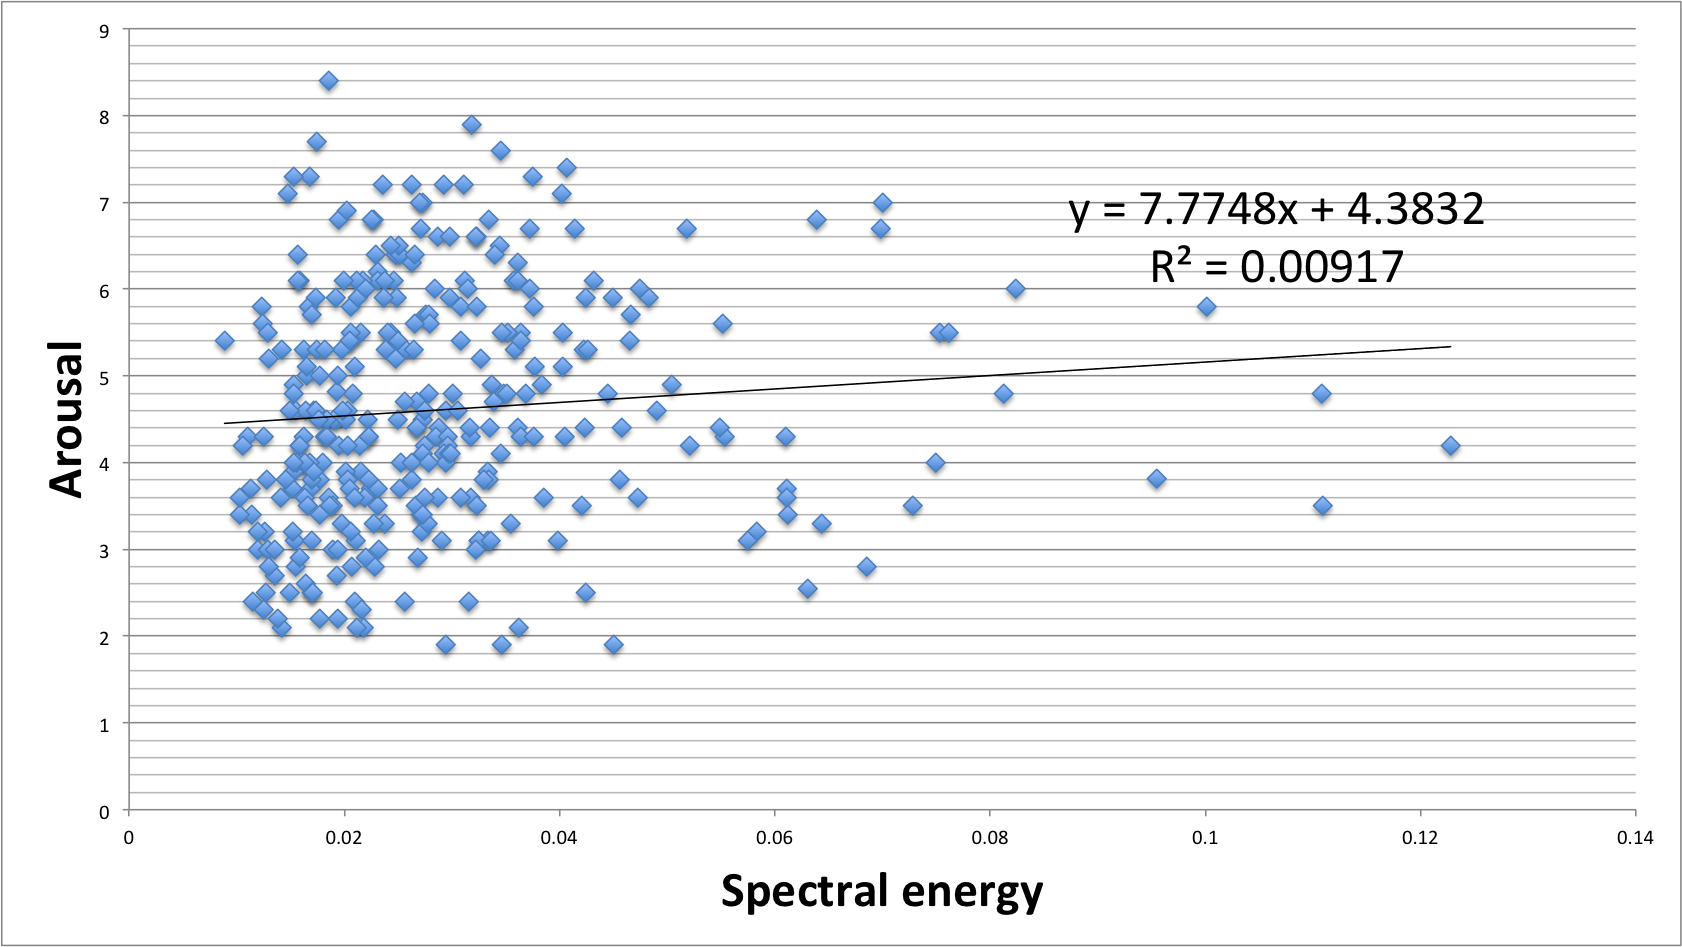
\includegraphics[width=\textwidth]{Figures/spectralenergy-arousal}
			   \vspace{20pt}
        \end{subfigure}
        \begin{subfigure}[b]{0.48\textwidth}
                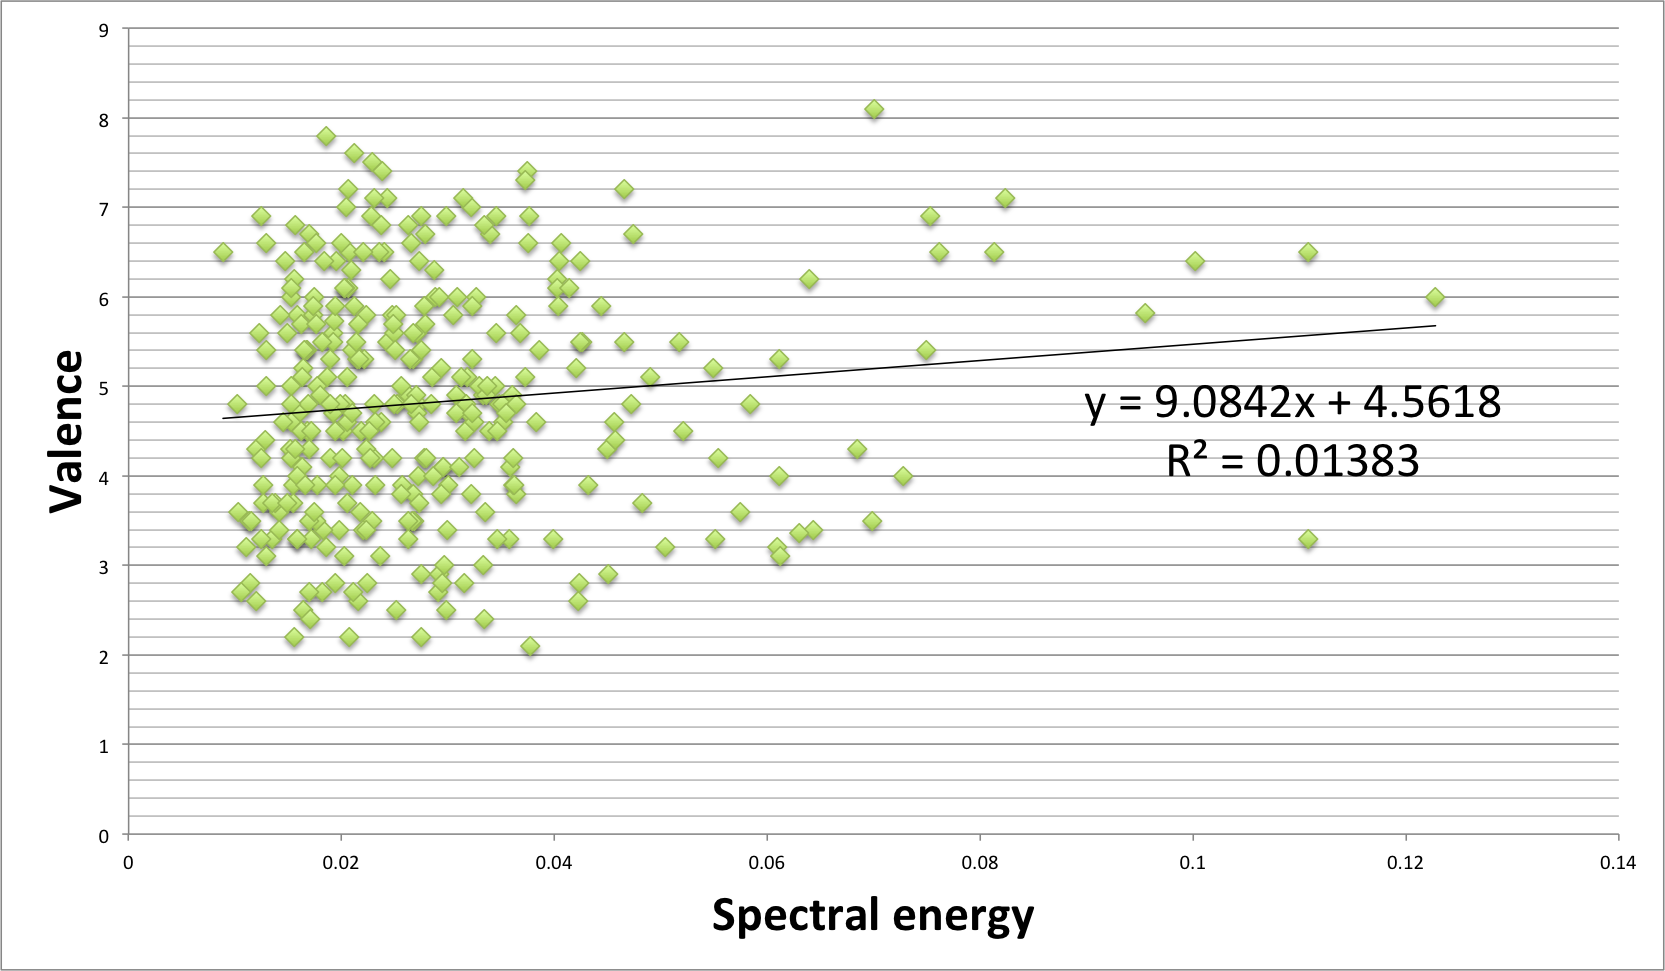
\includegraphics[width=\textwidth]{Figures/spectralenergy-valence}
                  \vspace{20pt}
        \end{subfigure}        
        
        \centering
        \begin{subfigure}[b]{0.48\textwidth}
                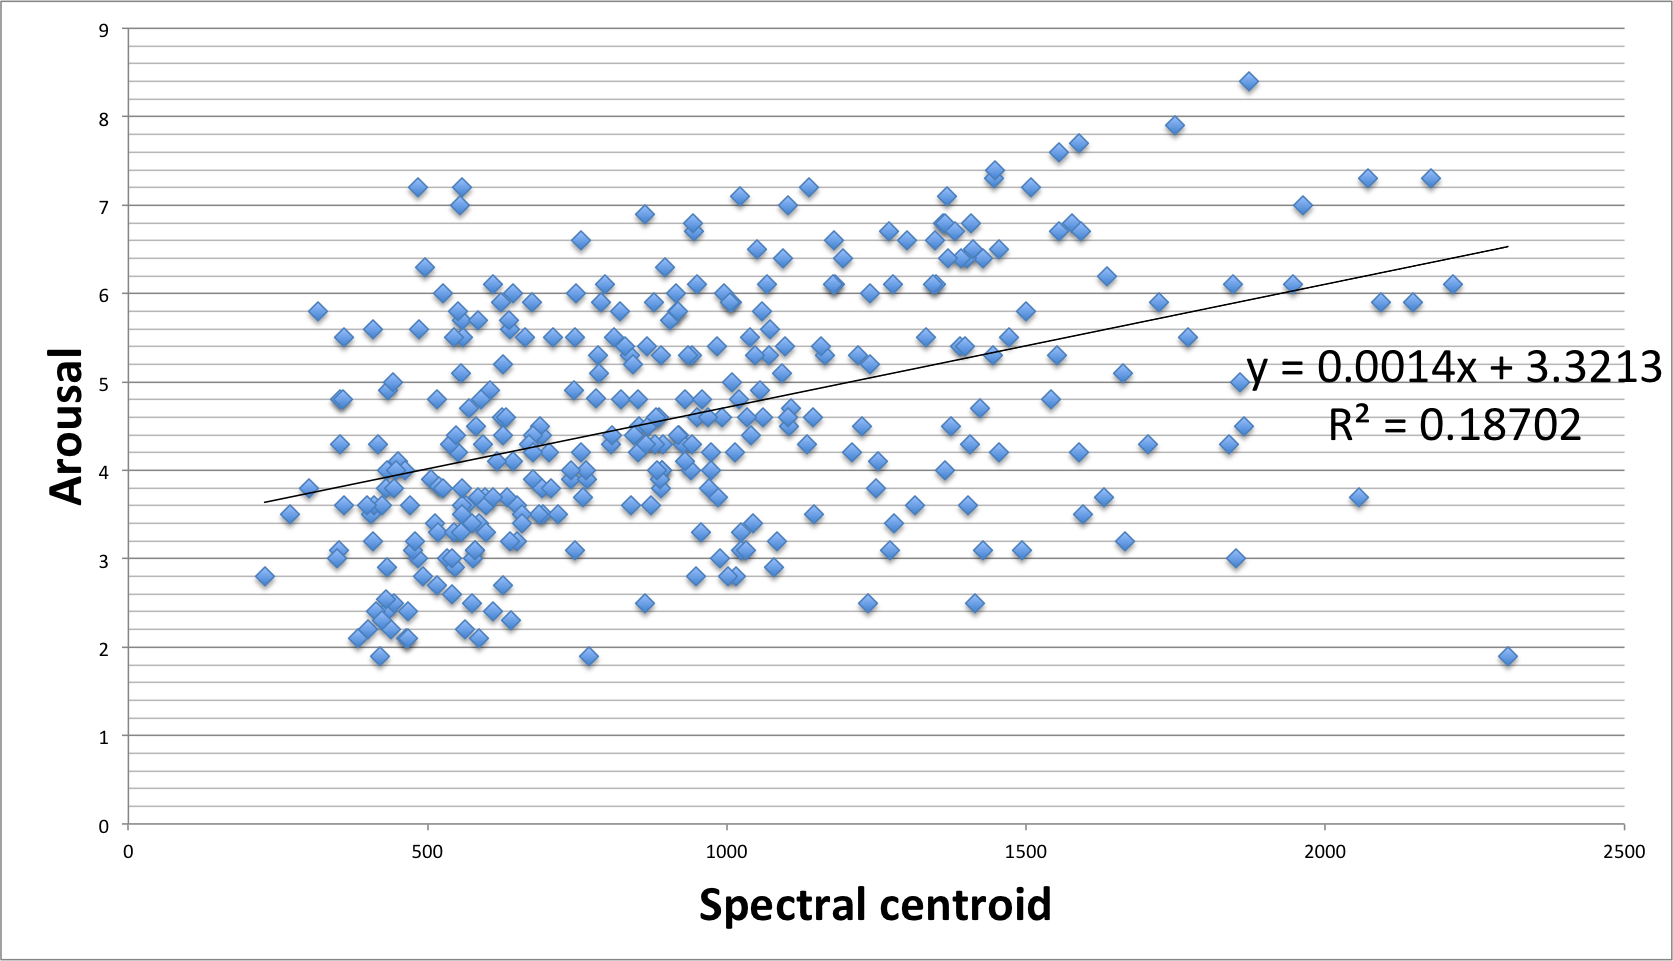
\includegraphics[width=\textwidth]{Figures/spectralcentroid-arousal}
                \vspace{20pt}
        \end{subfigure}
        \begin{subfigure}[b]{0.48\textwidth}
                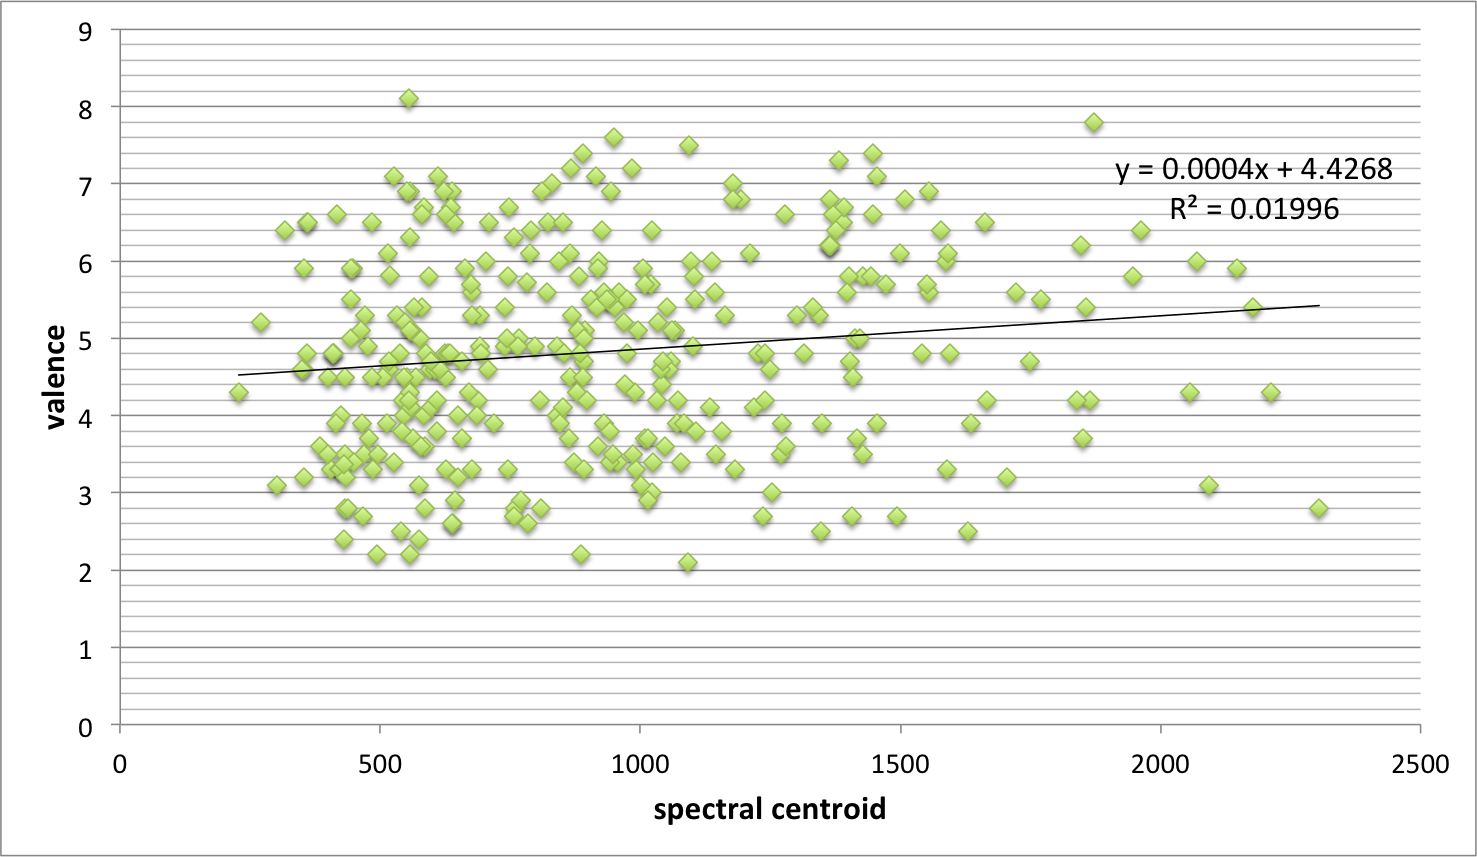
\includegraphics[width=\textwidth]{Figures/spectralcentroid-valence}
                \vspace{20pt}
        \end{subfigure}

\end{figure}
\begin{figure}
 
         \centering
        \begin{subfigure}[b]{0.48\textwidth}
                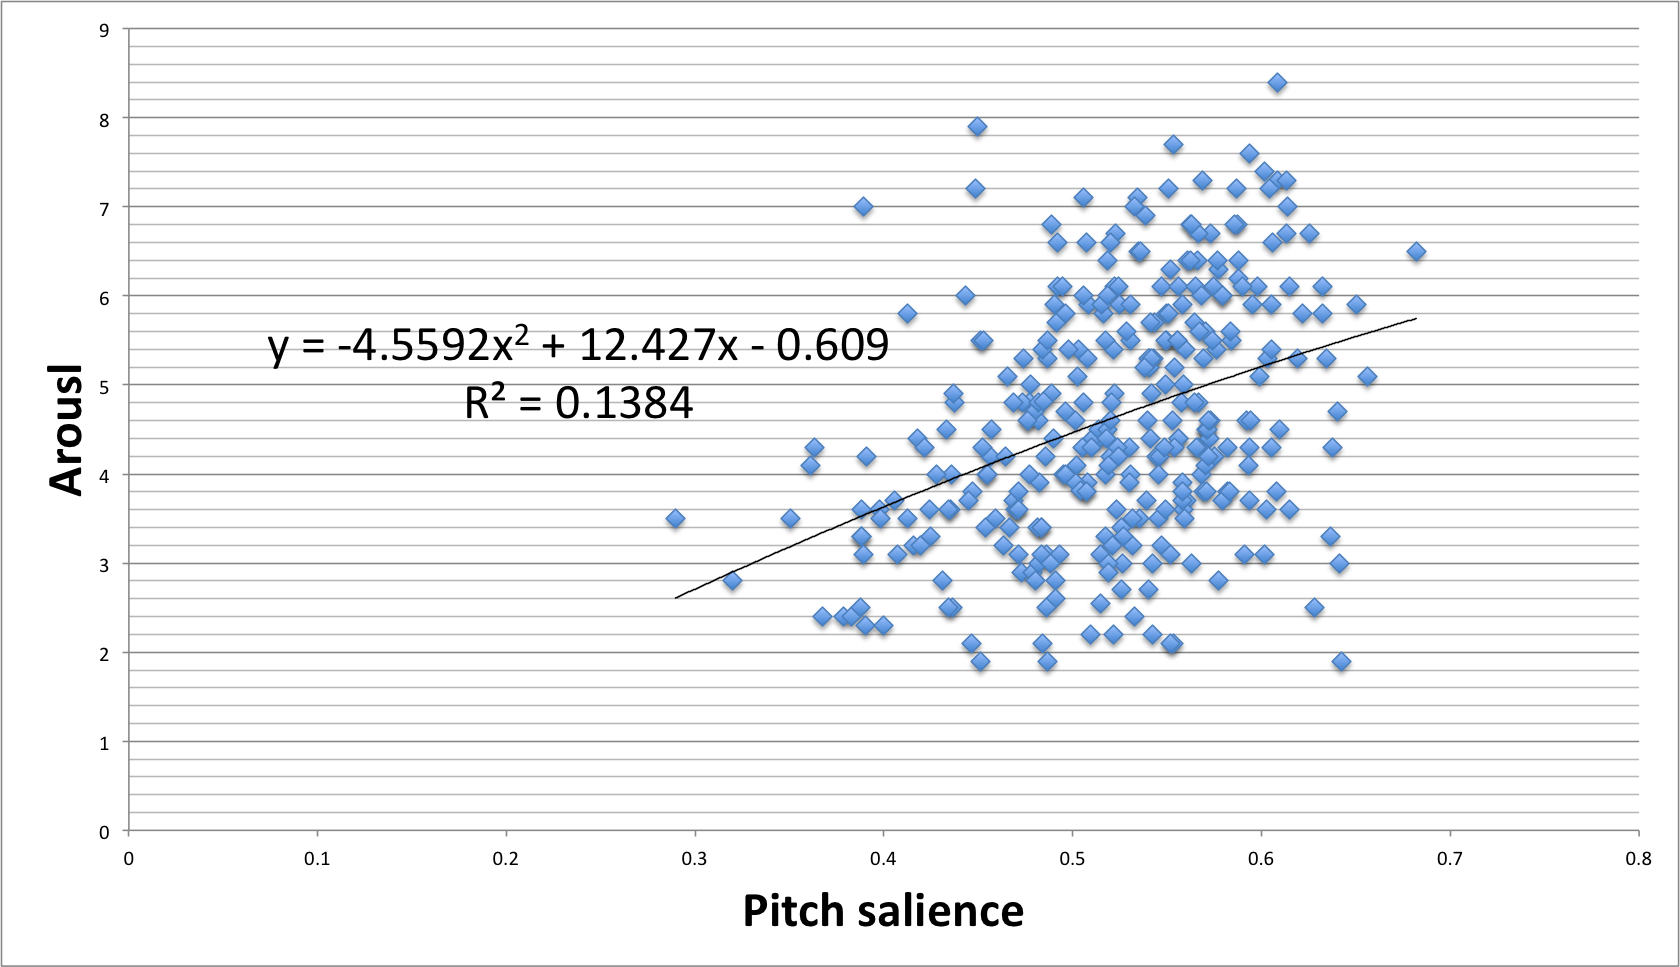
\includegraphics[width=\textwidth]{Figures/pitchsalience-arousal}
			   \vspace{20pt}
        \end{subfigure}
        \begin{subfigure}[b]{0.48\textwidth}
                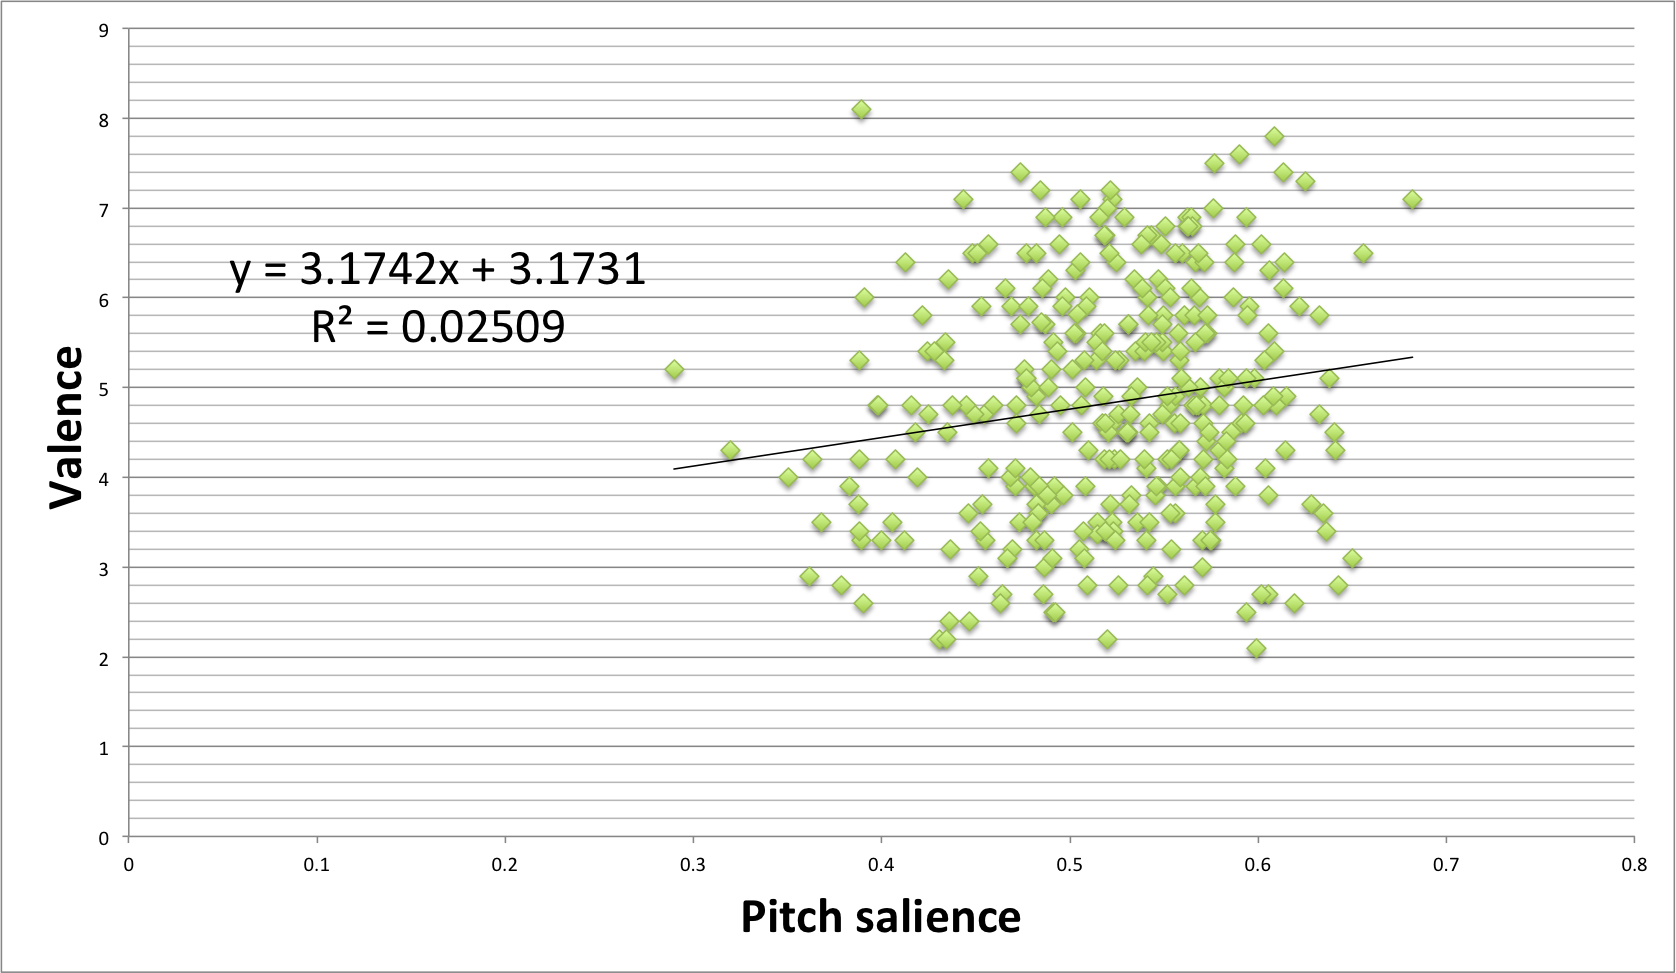
\includegraphics[width=\textwidth]{Figures/pitchsalience-valence}
                  \vspace{20pt}
        \end{subfigure}

          \centering
        \begin{subfigure}[b]{0.48\textwidth}
                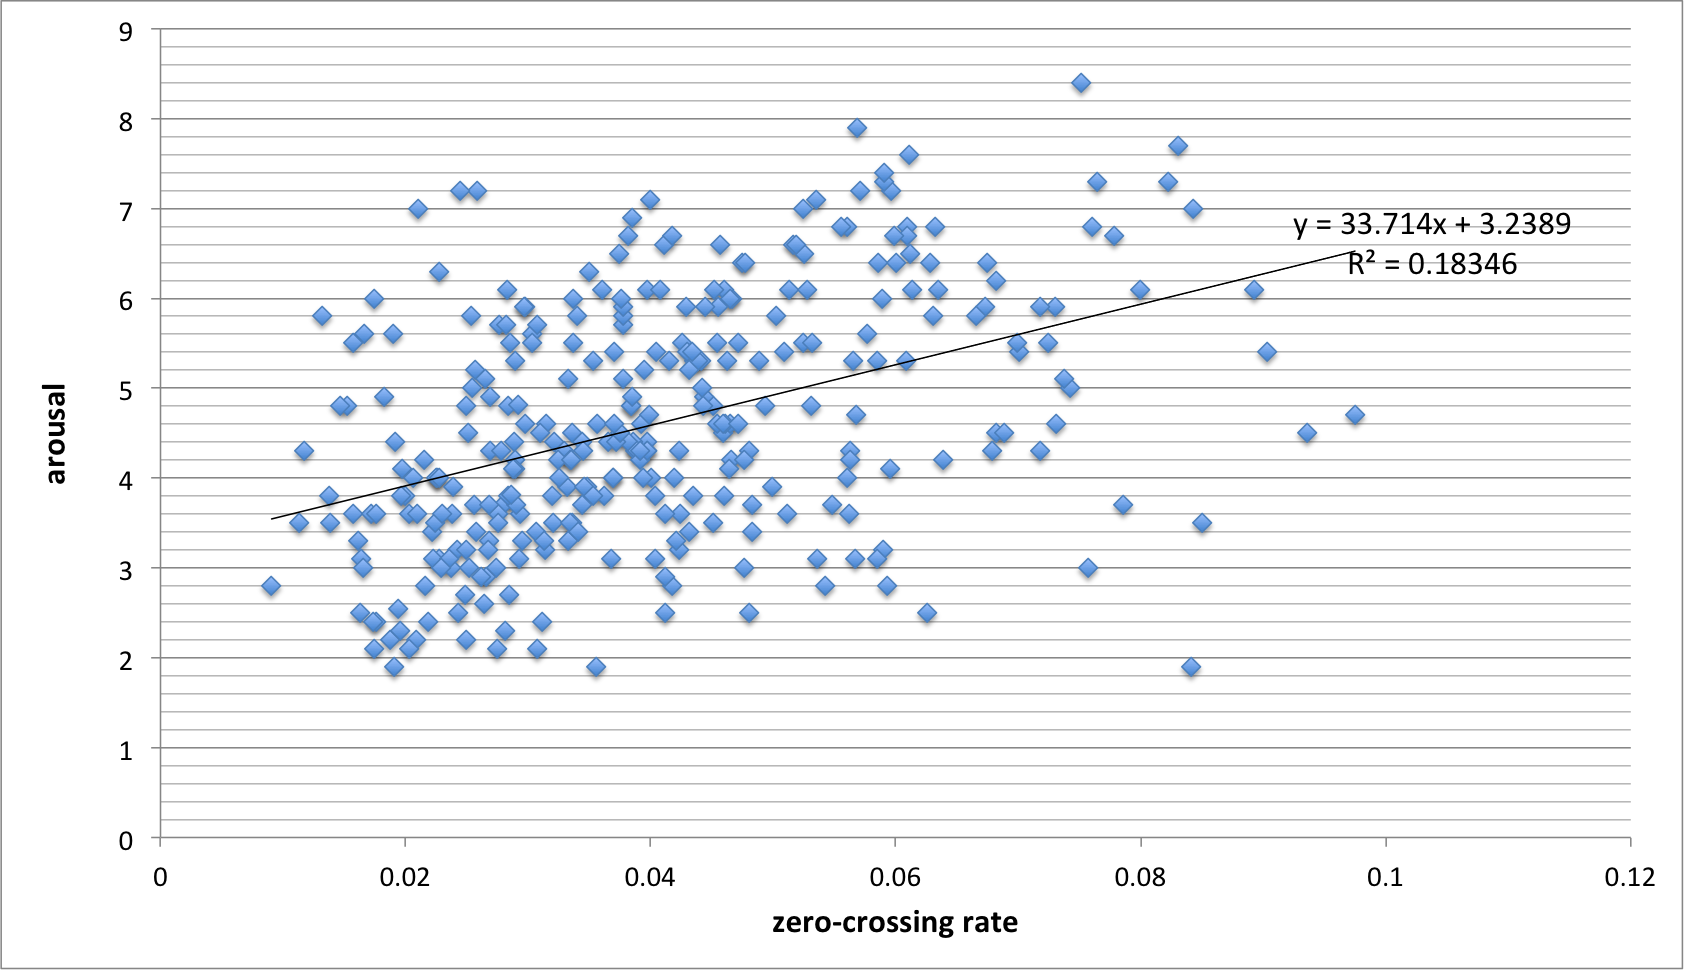
\includegraphics[width=\textwidth]{Figures/zerocrossing-arousal}
			   \vspace{20pt}
        \end{subfigure}
        \begin{subfigure}[b]{0.48\textwidth}
                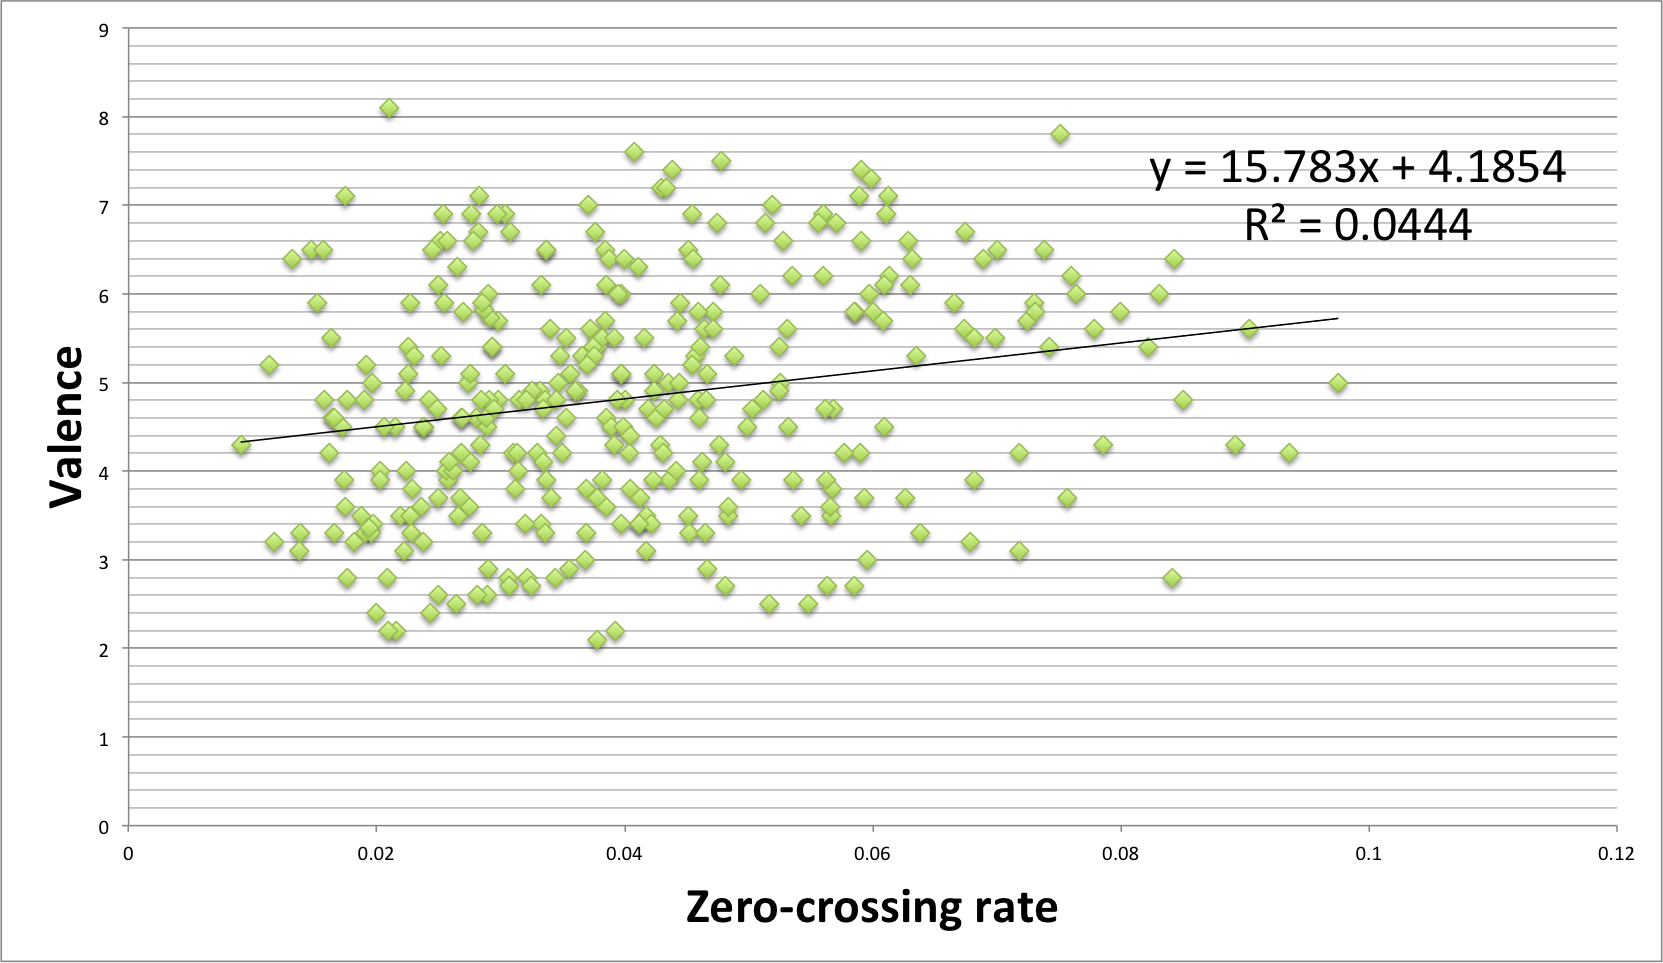
\includegraphics[width=\textwidth]{Figures/zerocrossing-valence}
                  \vspace{20pt}
        \end{subfigure}
        
         \centering
        \begin{subfigure}[b]{0.48\textwidth}
                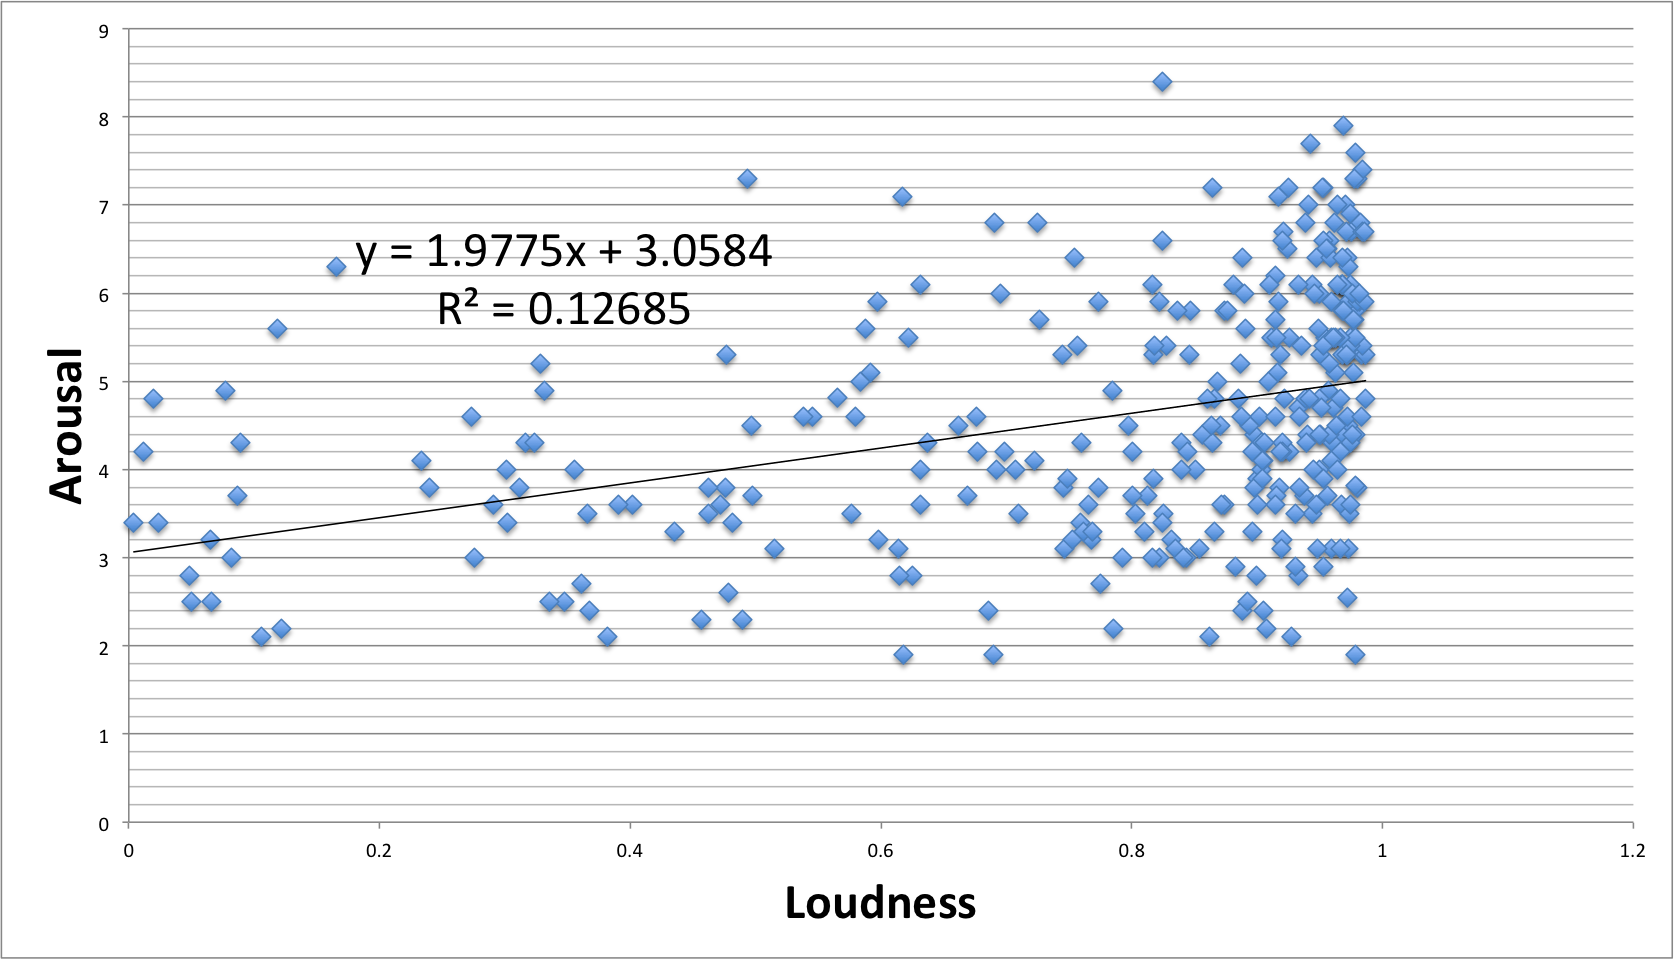
\includegraphics[width=\textwidth]{Figures/loudness-arousal}
			   \vspace{20pt}
        \end{subfigure}
        \begin{subfigure}[b]{0.48\textwidth}
                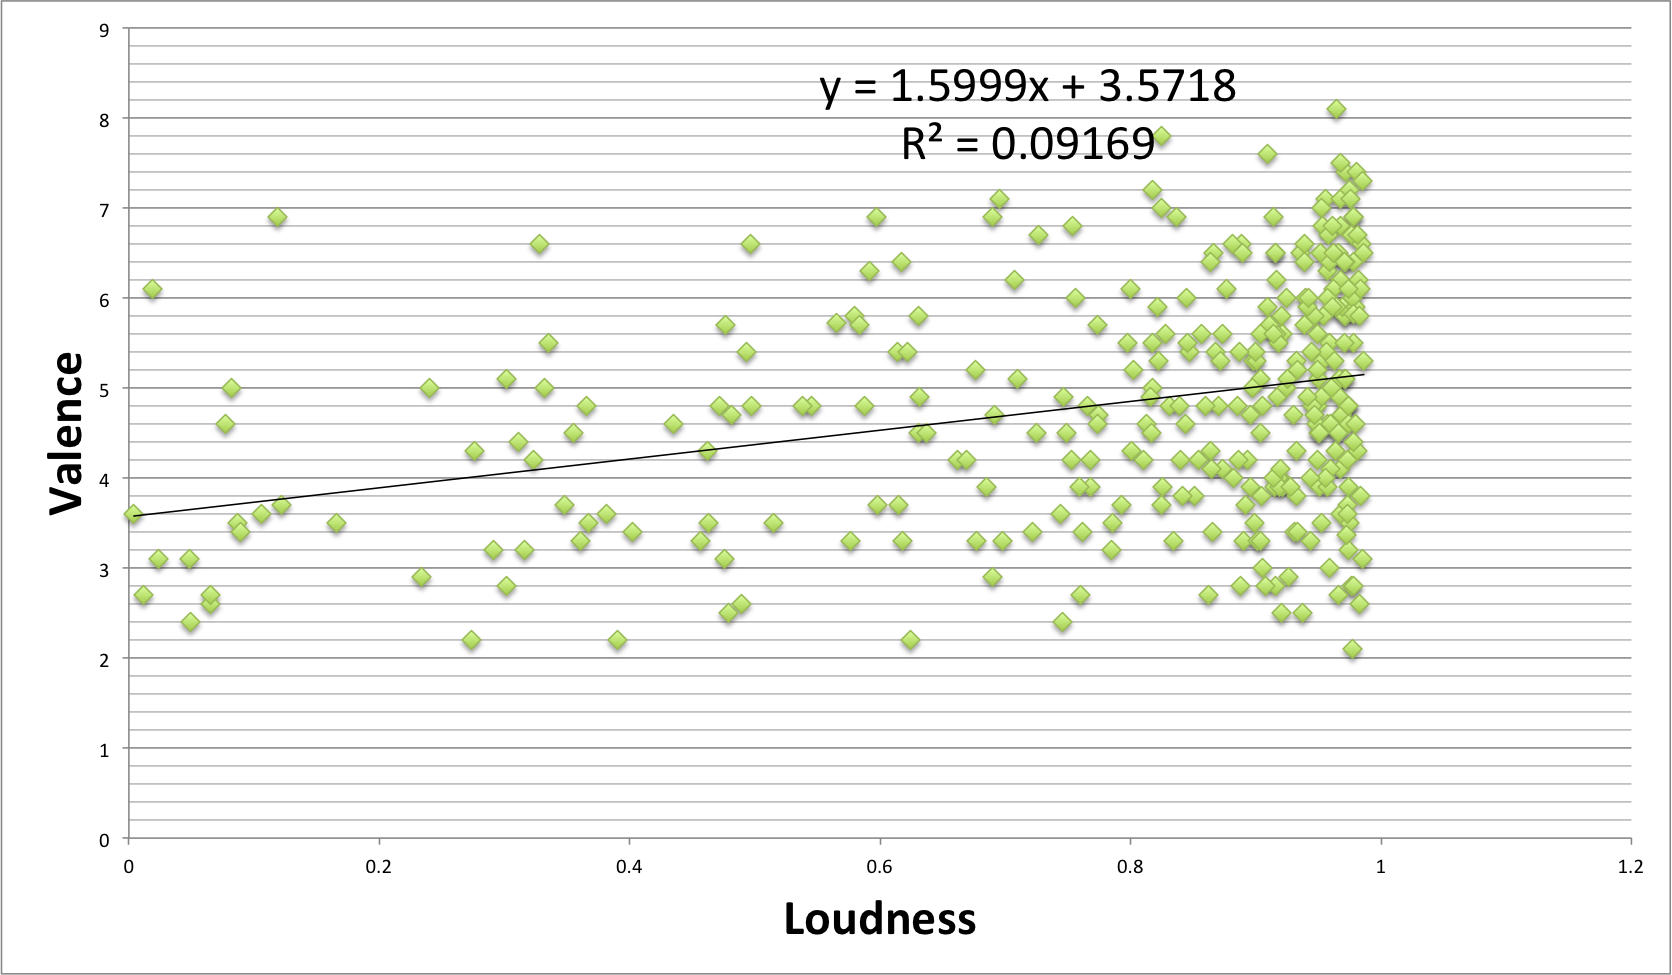
\includegraphics[width=\textwidth]{Figures/loudness-valence}
                  \vspace{20pt}
        \end{subfigure}
        
             \centering
        \begin{subfigure}[b]{0.48\textwidth}
                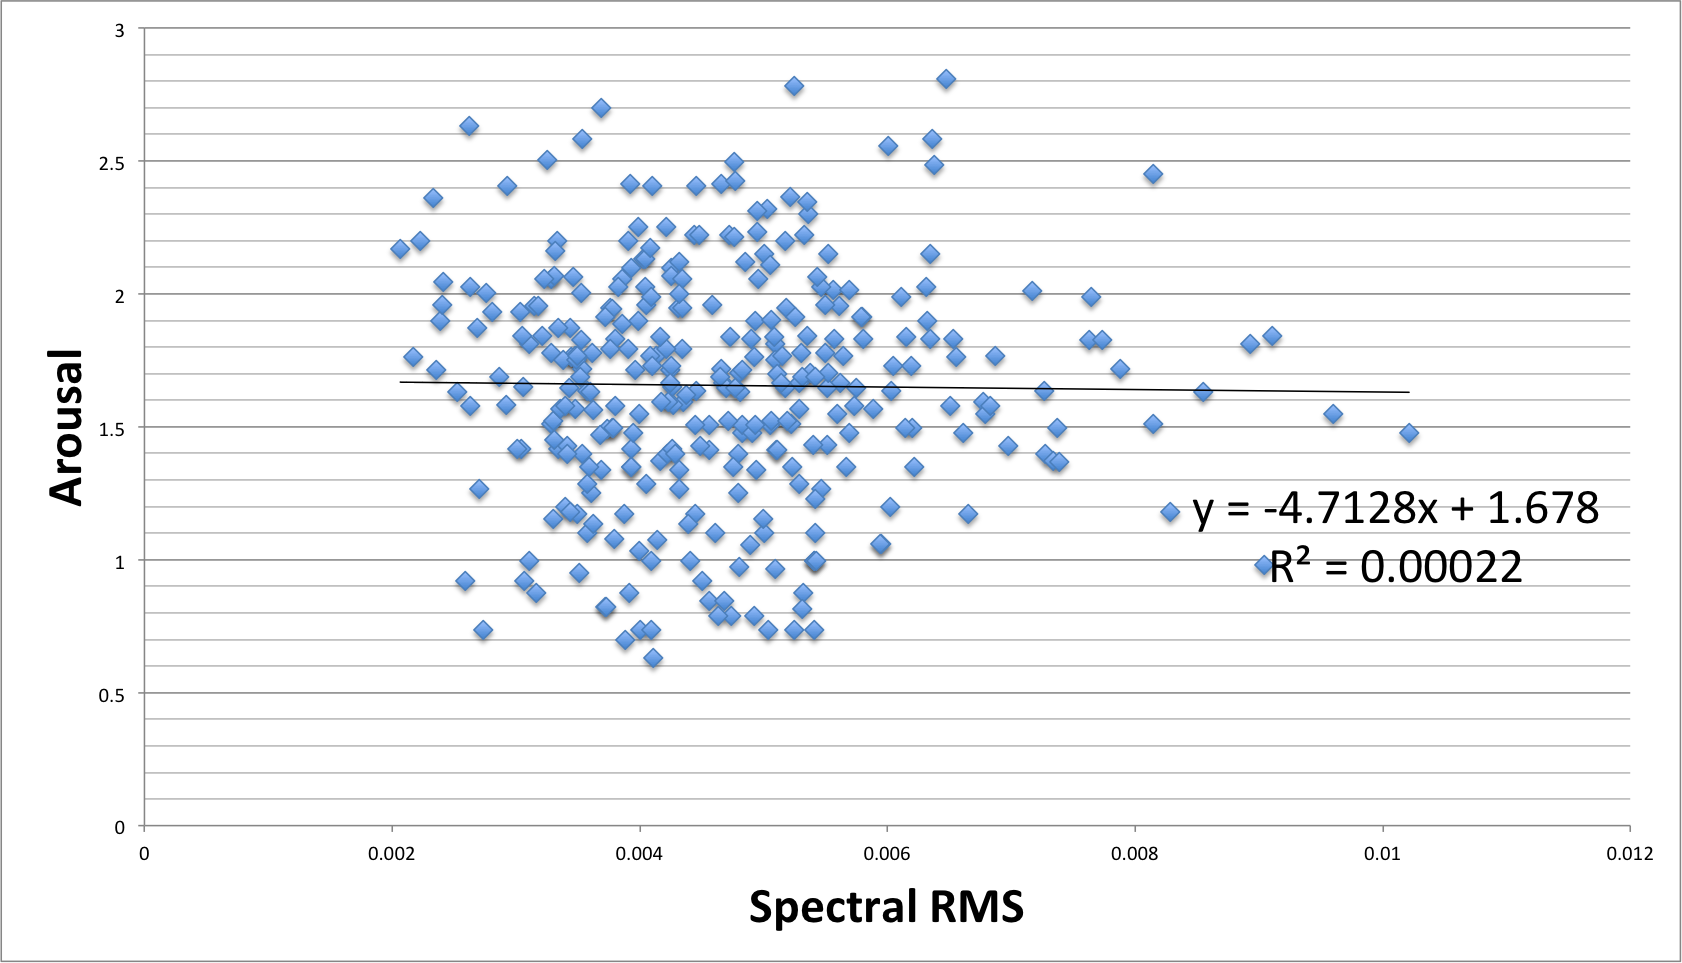
\includegraphics[width=\textwidth]{Figures/spectralrms-arousal}
			   \vspace{20pt}
        \end{subfigure}
        \begin{subfigure}[b]{0.48\textwidth}
                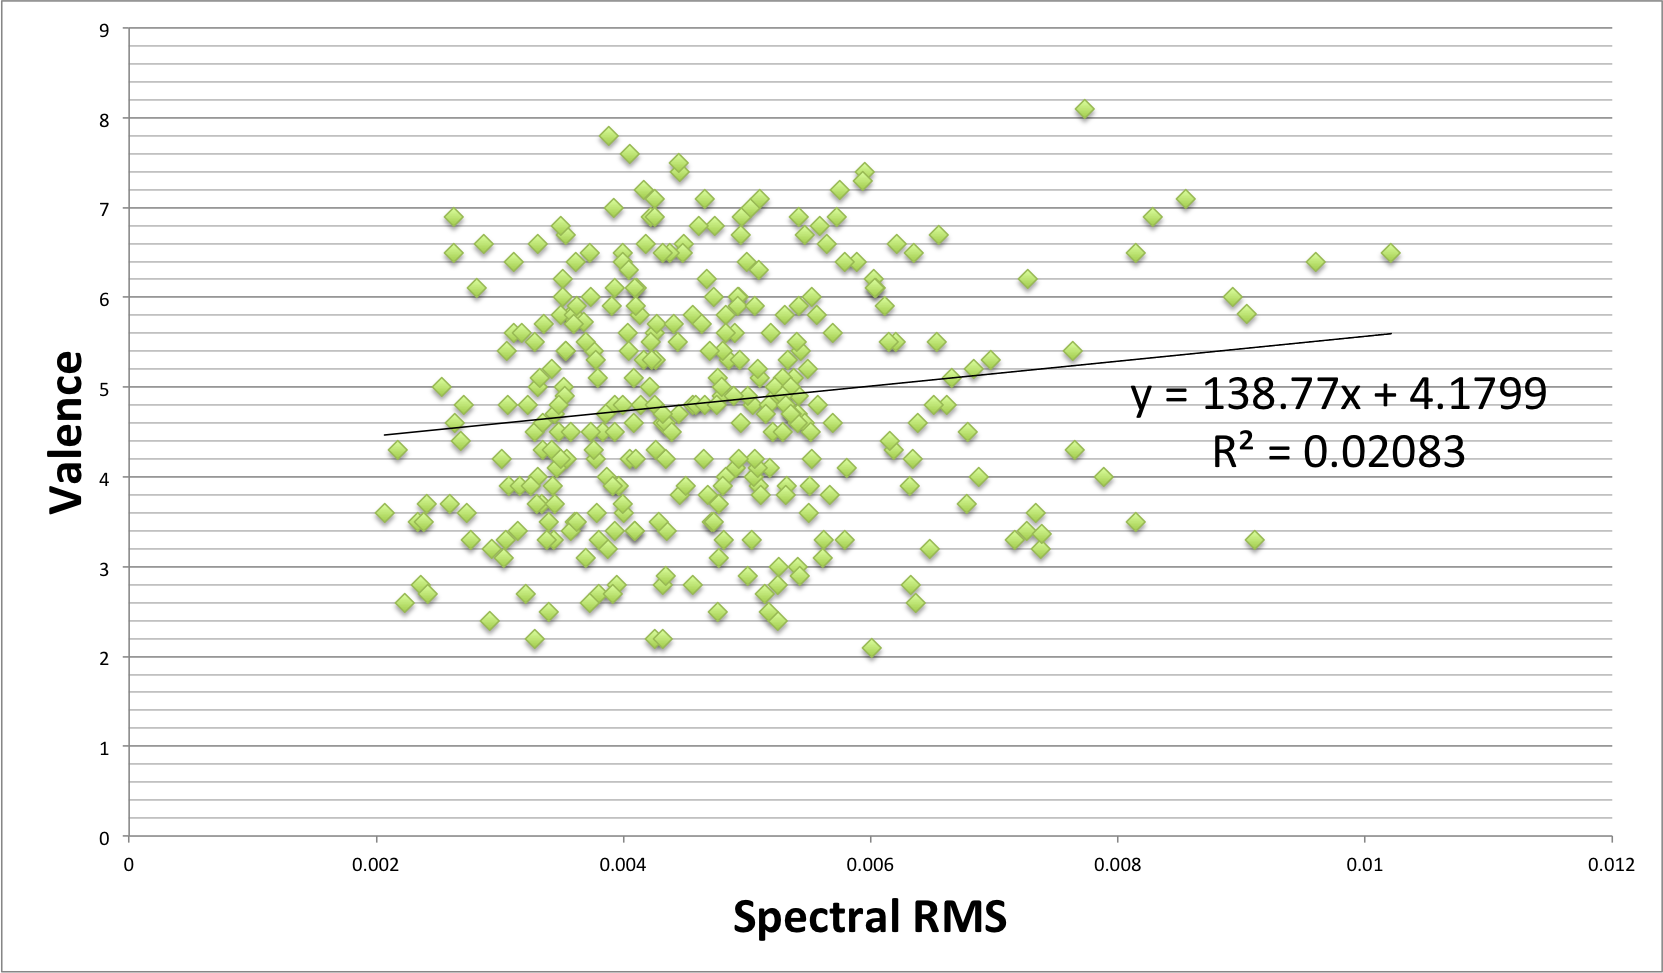
\includegraphics[width=\textwidth]{Figures/spectralrms-valence}
                  \vspace{20pt}
        \end{subfigure}
        
\end{figure}

\begin{figure}  
         \centering
        \begin{subfigure}[b]{0.48\textwidth}
                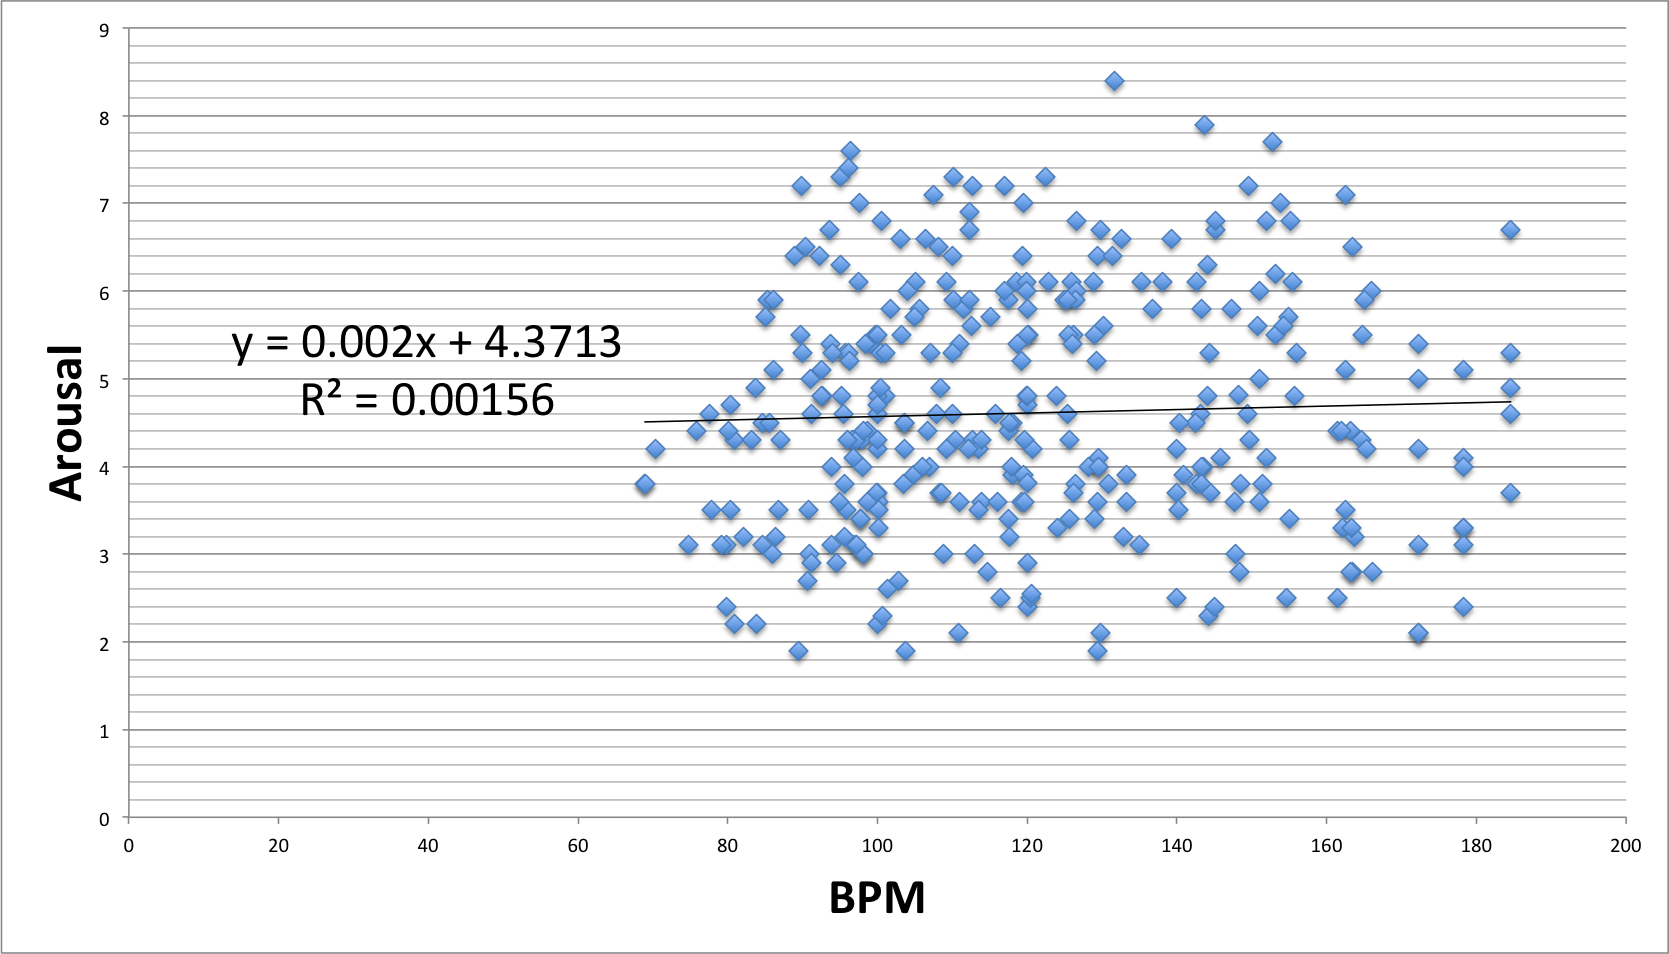
\includegraphics[width=\textwidth]{Figures/bpm-arousal}
			   \vspace{20pt}
        \end{subfigure}
        \begin{subfigure}[b]{0.48\textwidth}
                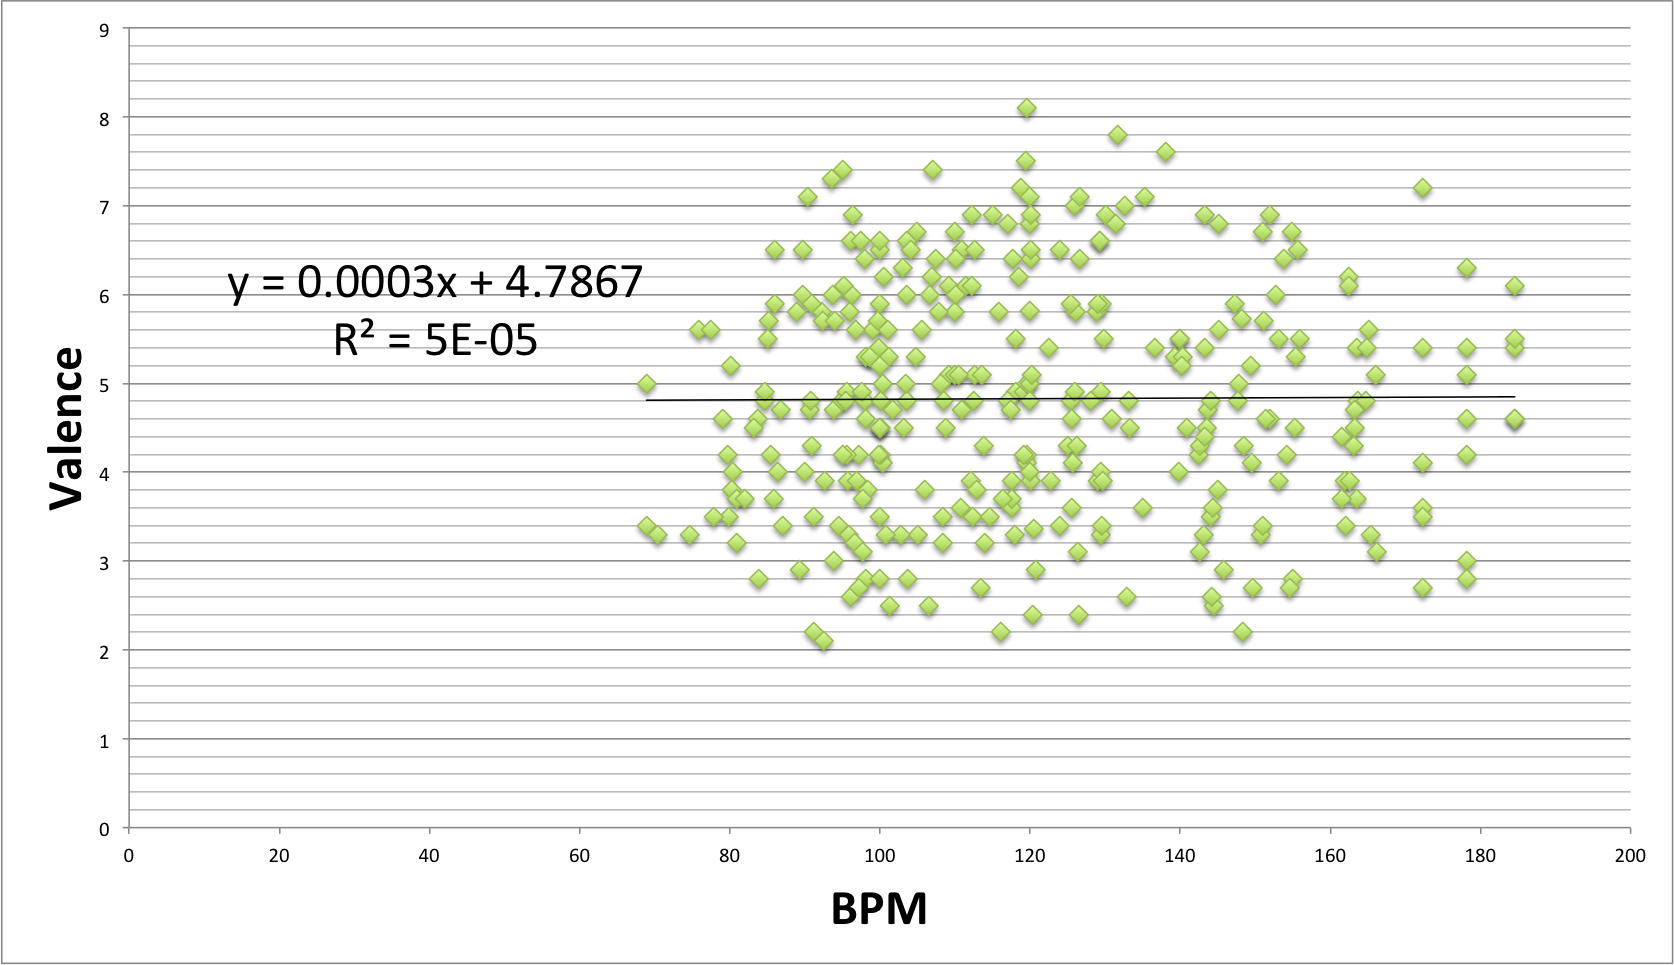
\includegraphics[width=\textwidth]{Figures/bpm-valence}
                  \vspace{20pt}
        \end{subfigure}
        
         \centering
        \begin{subfigure}[b]{0.48\textwidth}
                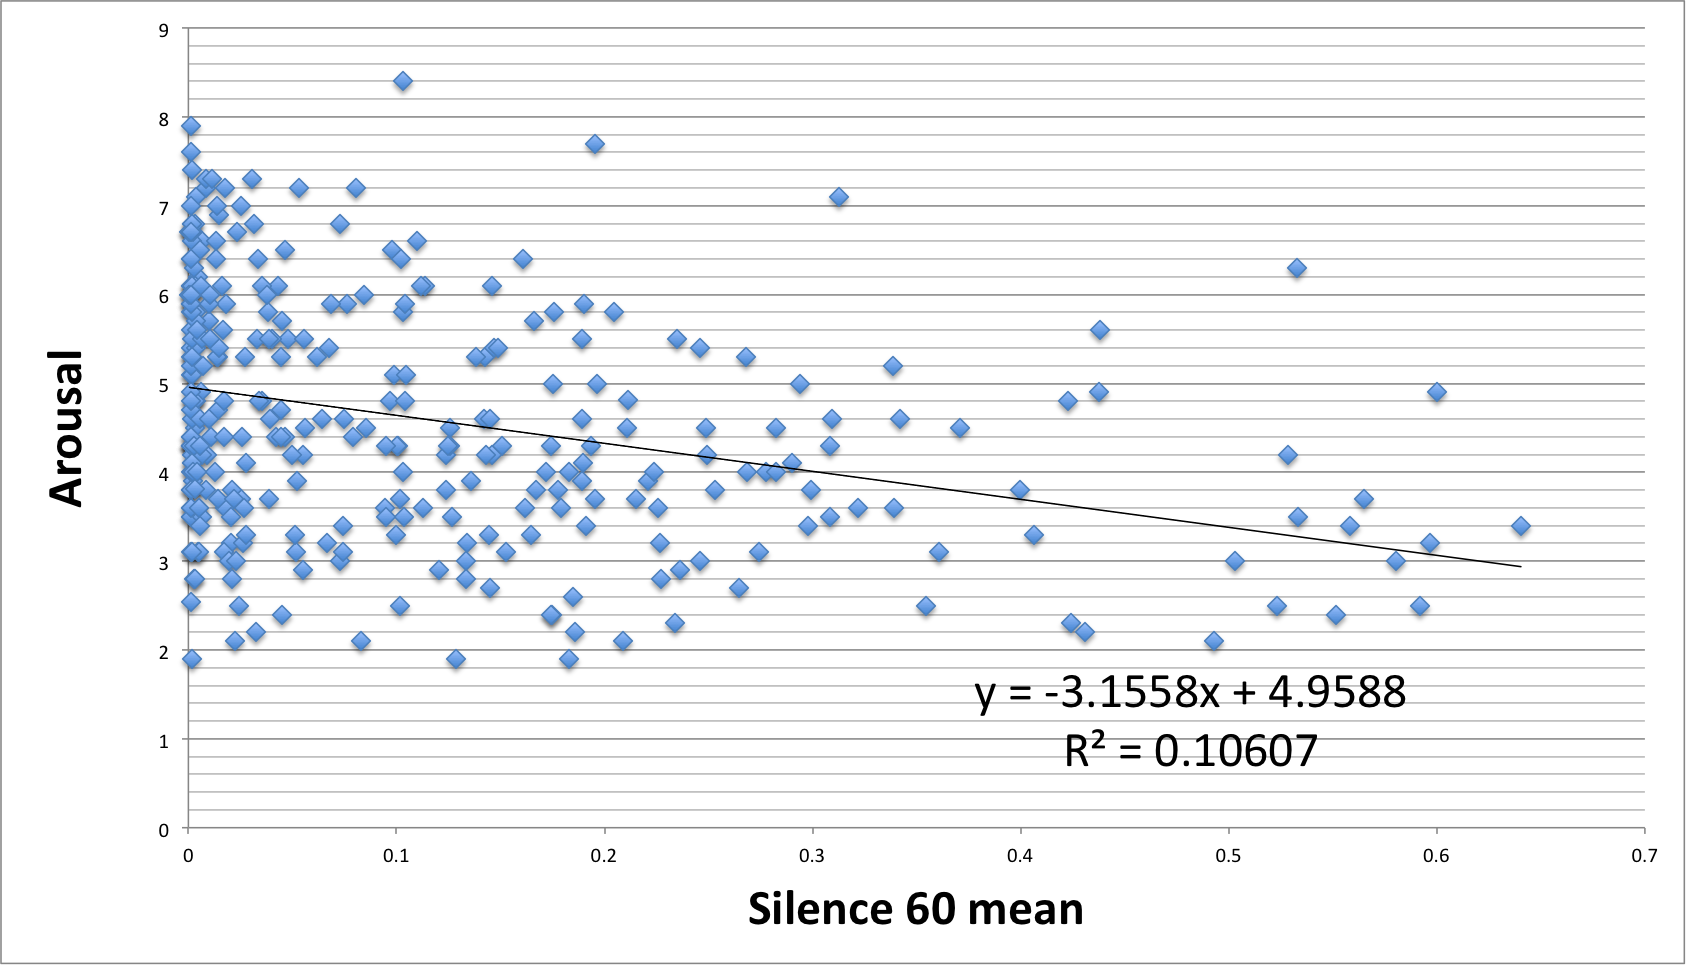
\includegraphics[width=\textwidth]{Figures/silence60mean-arousal}
			   \vspace{20pt}
        \end{subfigure}
        \begin{subfigure}[b]{0.48\textwidth}
                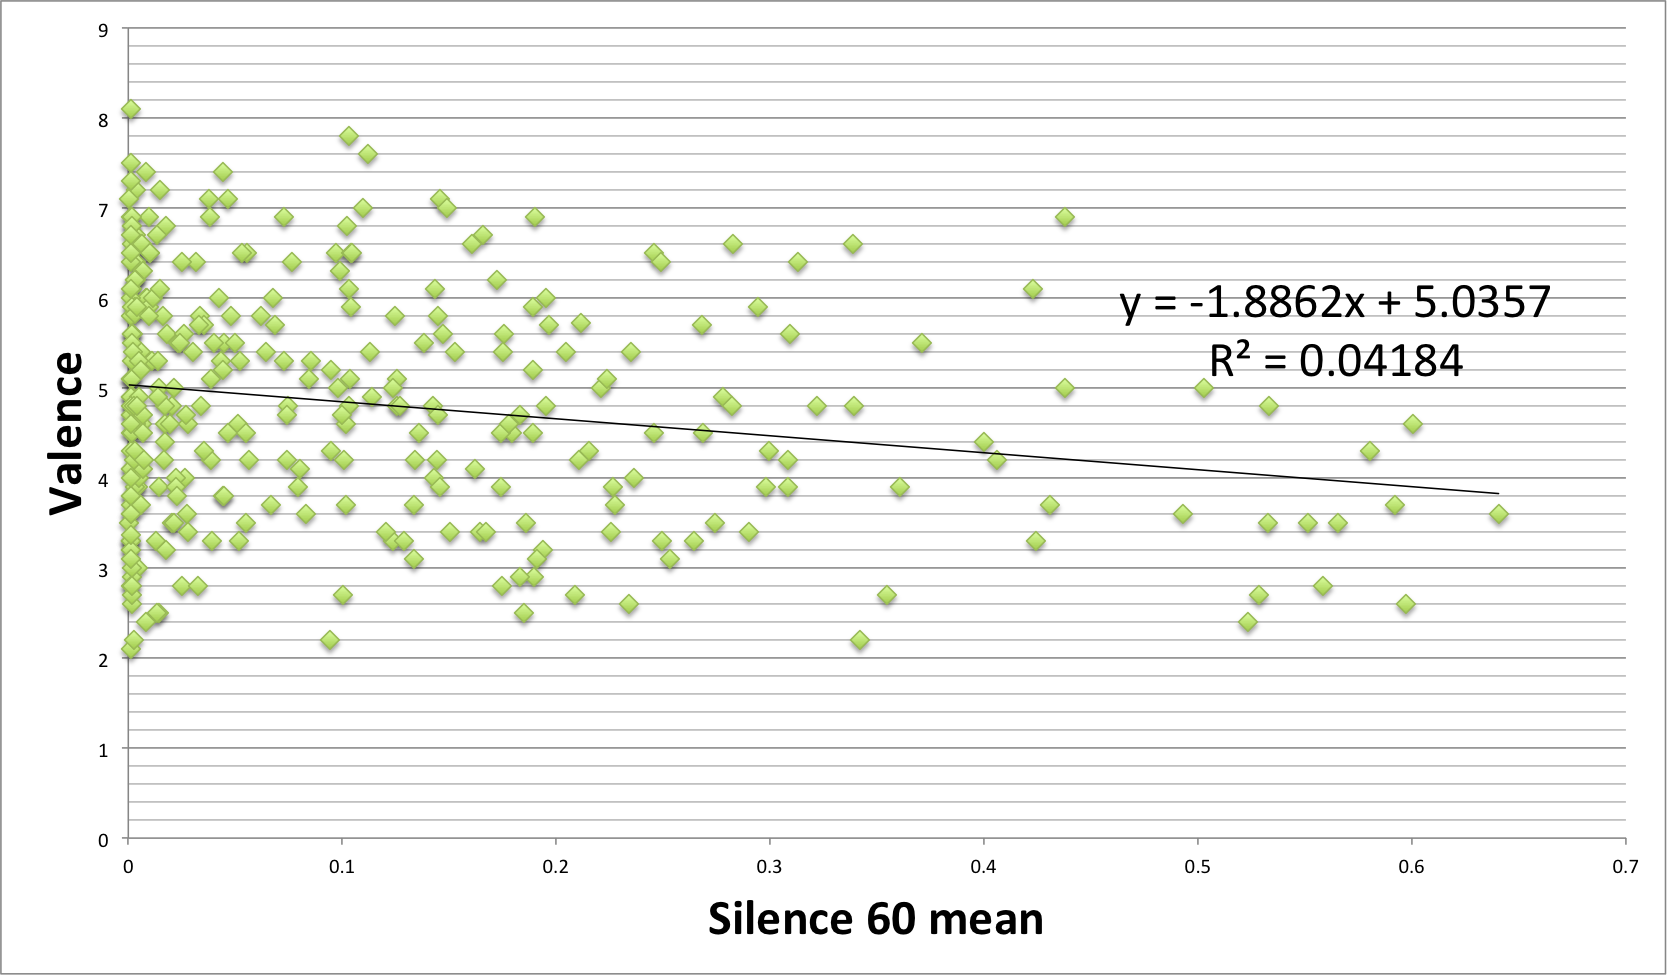
\includegraphics[width=\textwidth]{Figures/silence60mean-valence}
                  \vspace{20pt}
        \end{subfigure}

         \centering
        \begin{subfigure}[b]{0.48\textwidth}
                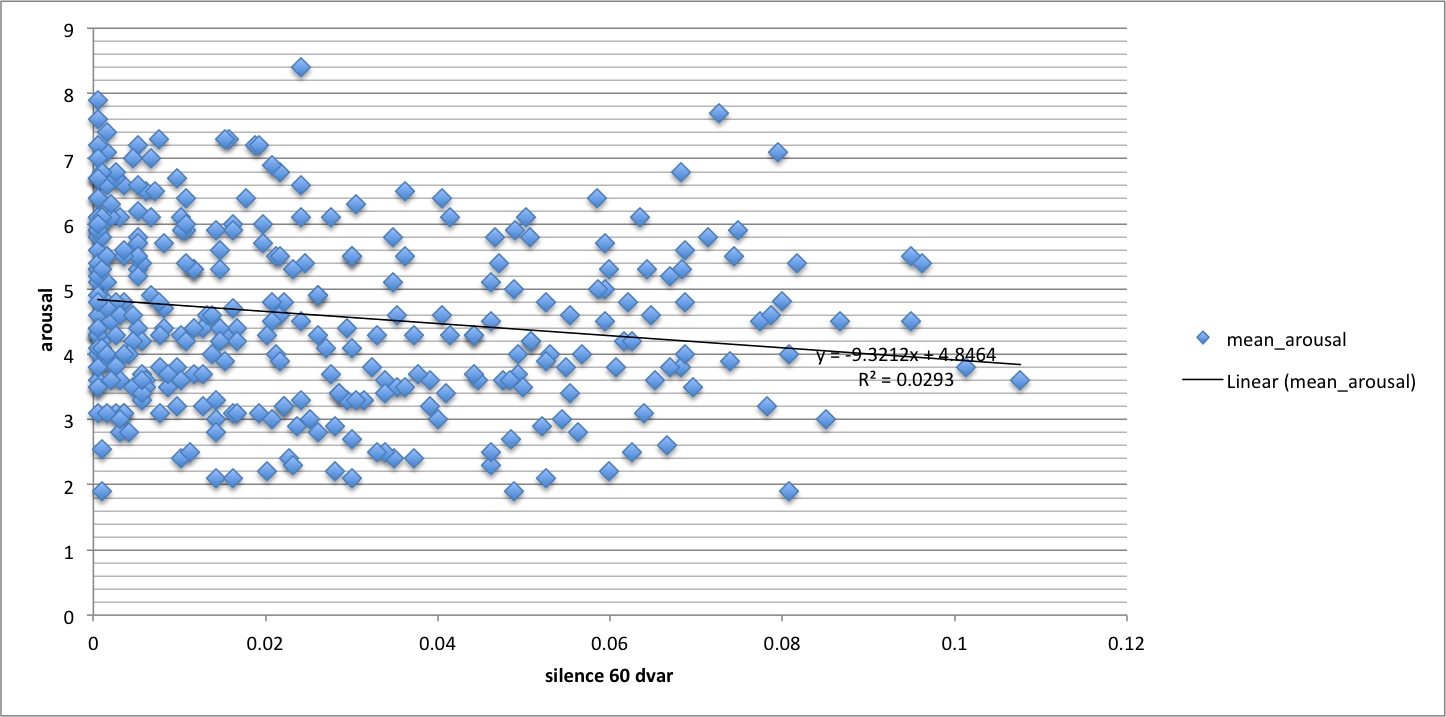
\includegraphics[width=\textwidth]{Figures/silence60dvar-arousal}
			   \vspace{20pt}
        \end{subfigure}
        \begin{subfigure}[b]{0.48\textwidth}
                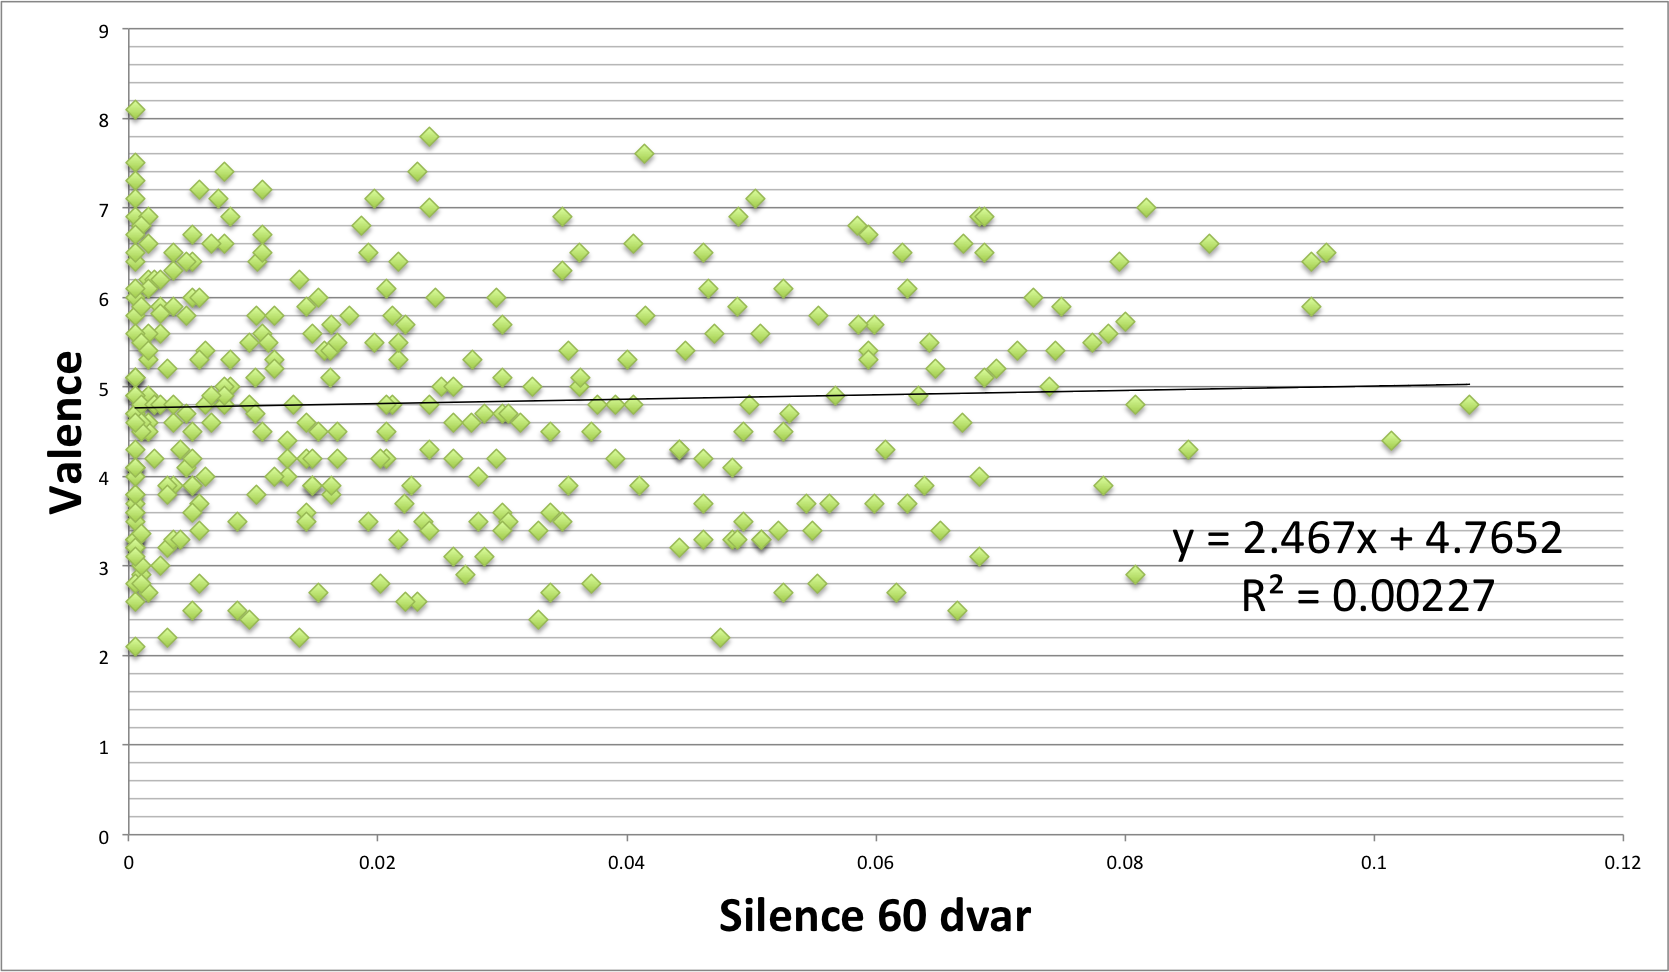
\includegraphics[width=\textwidth]{Figures/silence60dvar-valence}
                  \vspace{20pt}
        \end{subfigure}
        
         \centering
        \begin{subfigure}[b]{0.48\textwidth}
                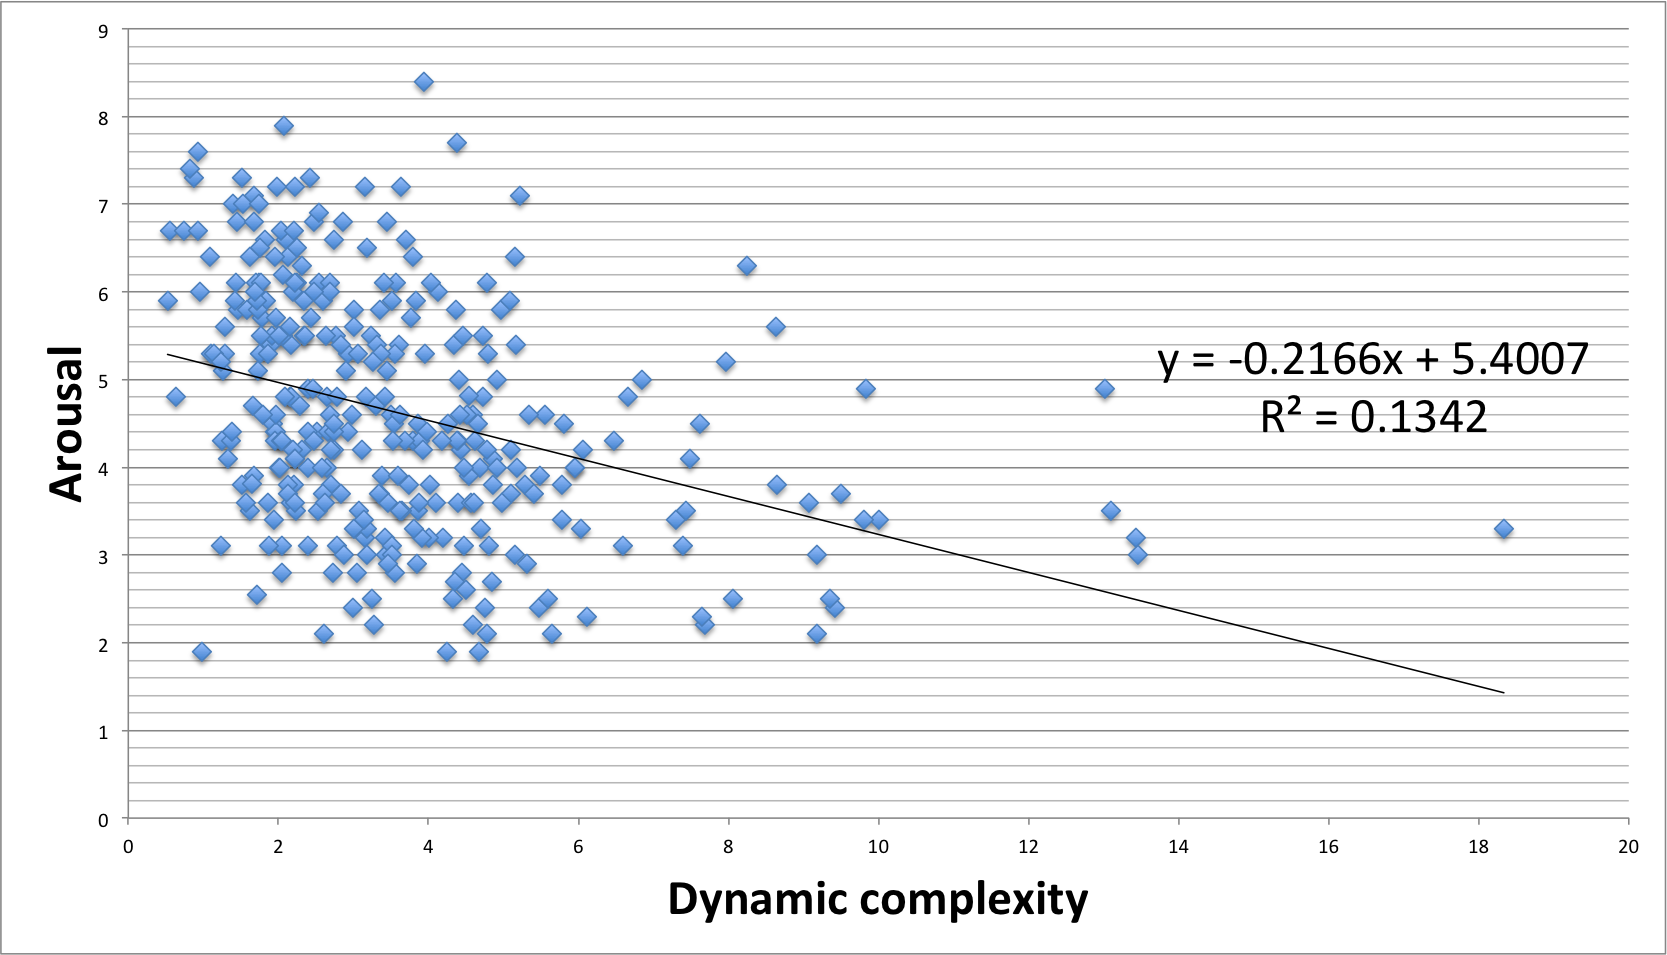
\includegraphics[width=\textwidth]{Figures/dynamiccomplexity-arousal}
			   \vspace{20pt}
        \end{subfigure}
        \begin{subfigure}[b]{0.48\textwidth}
                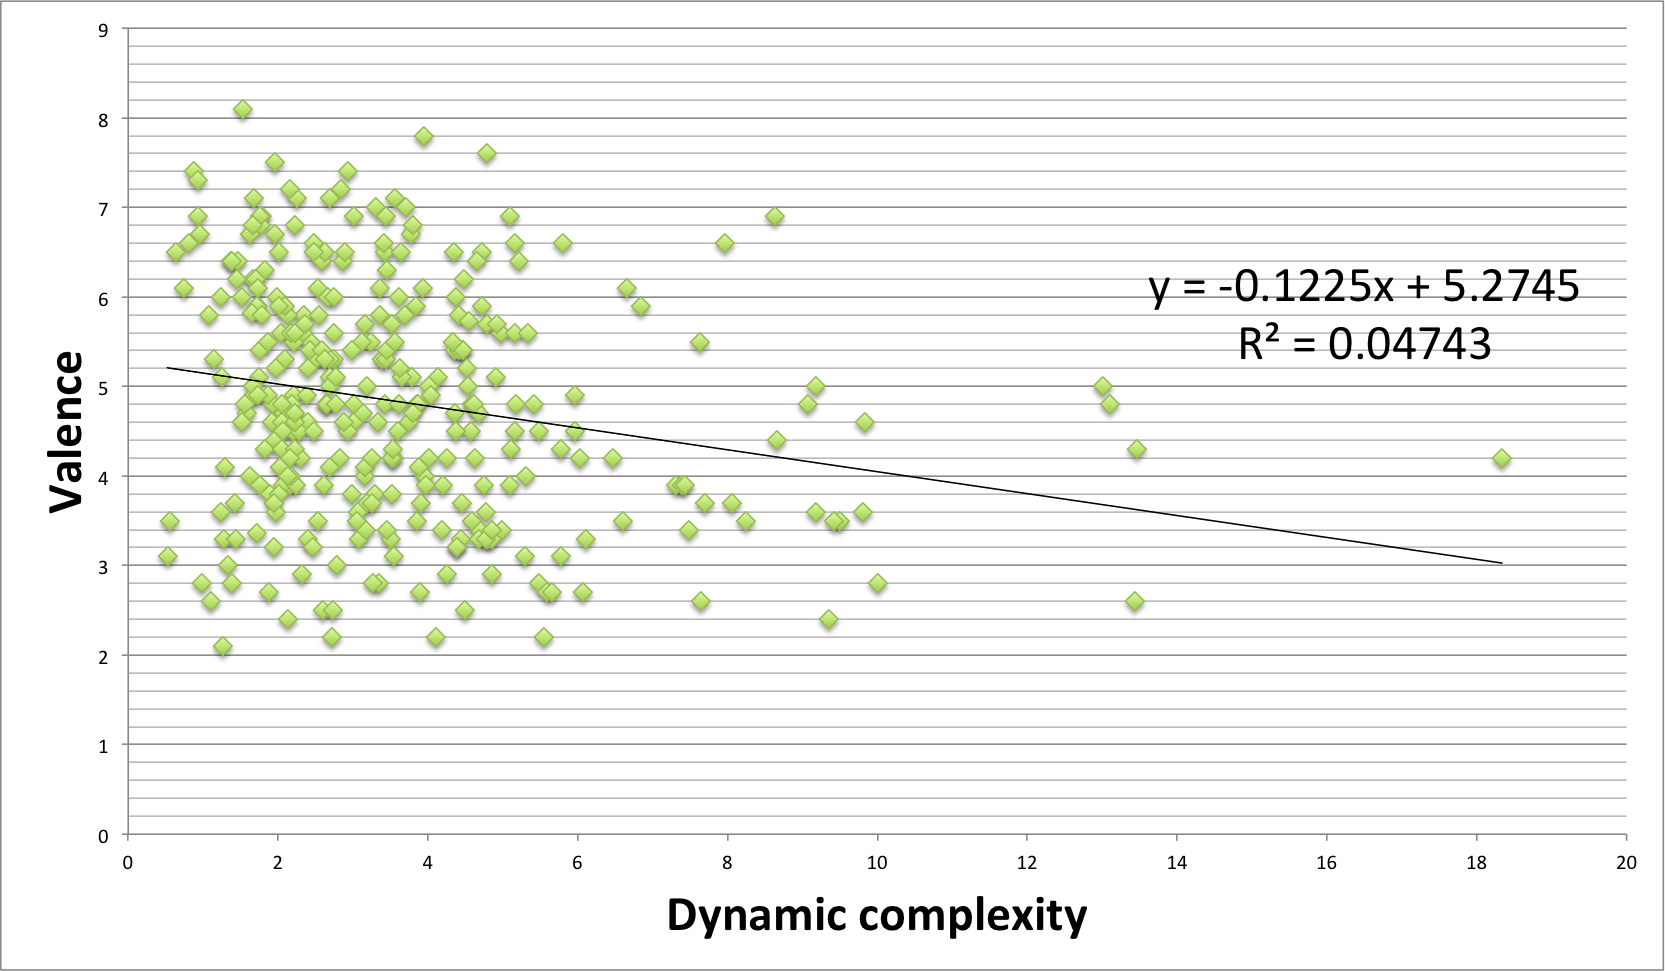
\includegraphics[width=\textwidth]{Figures/dynamiccomplexity-valence}
                  \vspace{20pt}
        \end{subfigure}
\end{figure}

\begin{figure}
         \centering
        \begin{subfigure}[b]{0.48\textwidth}
                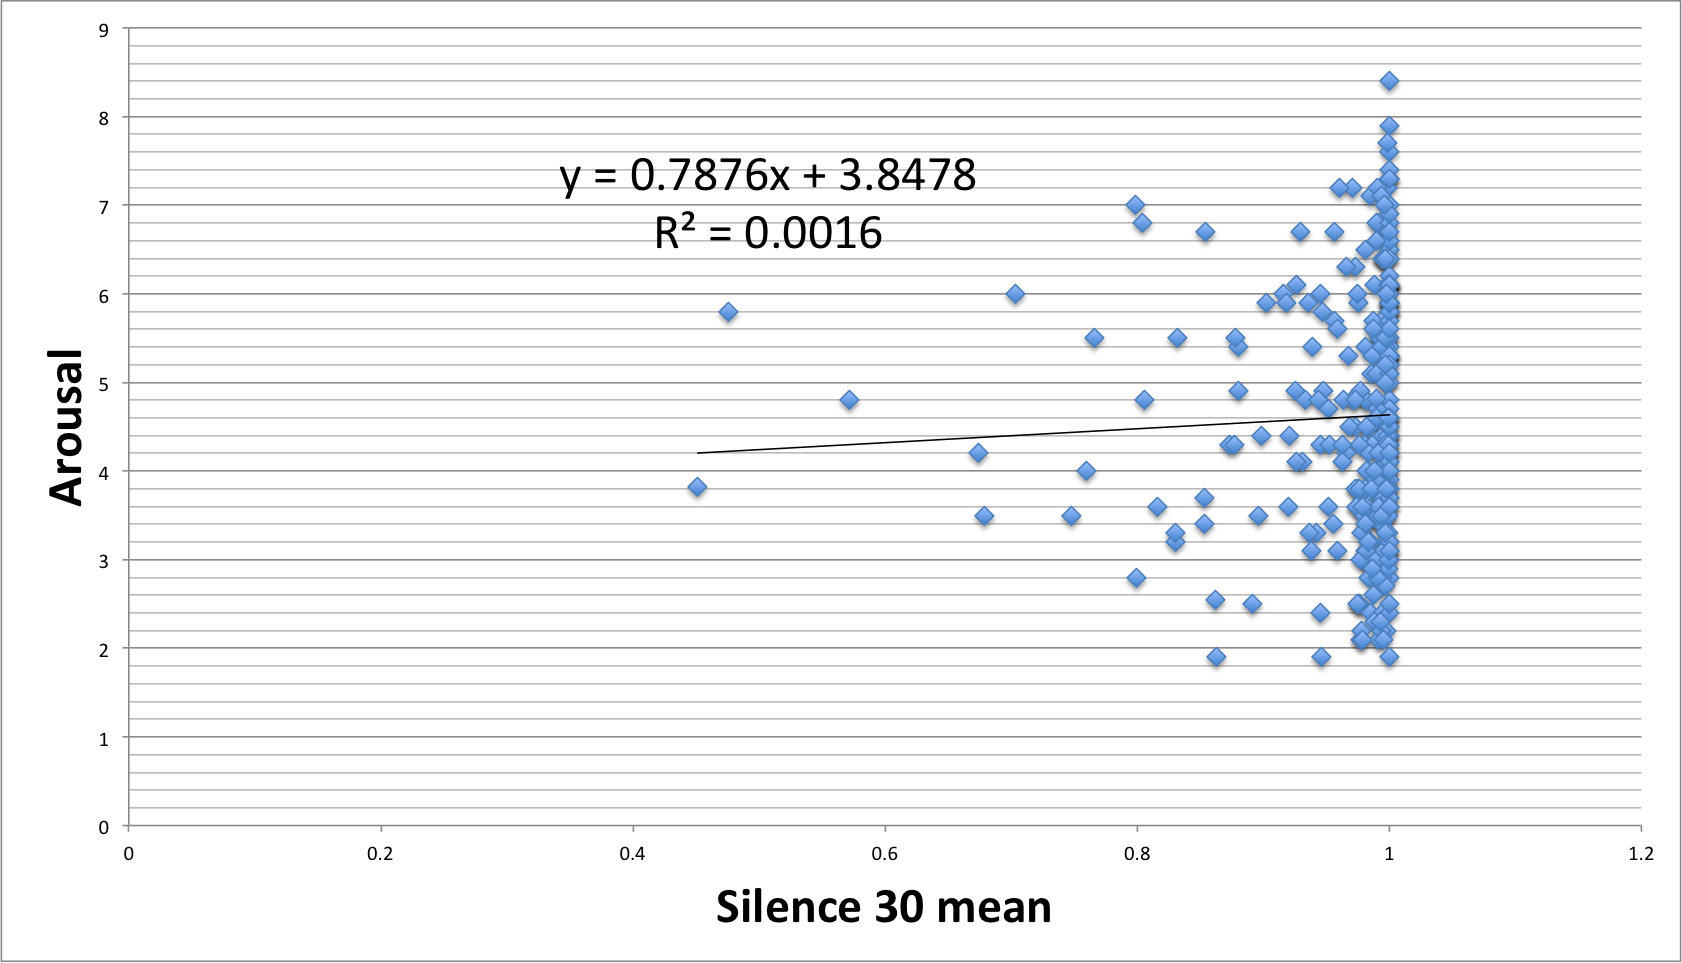
\includegraphics[width=\textwidth]{Figures/silence30mean-arousal}
			   \vspace{20pt}
        \end{subfigure}
        \begin{subfigure}[b]{0.48\textwidth}
                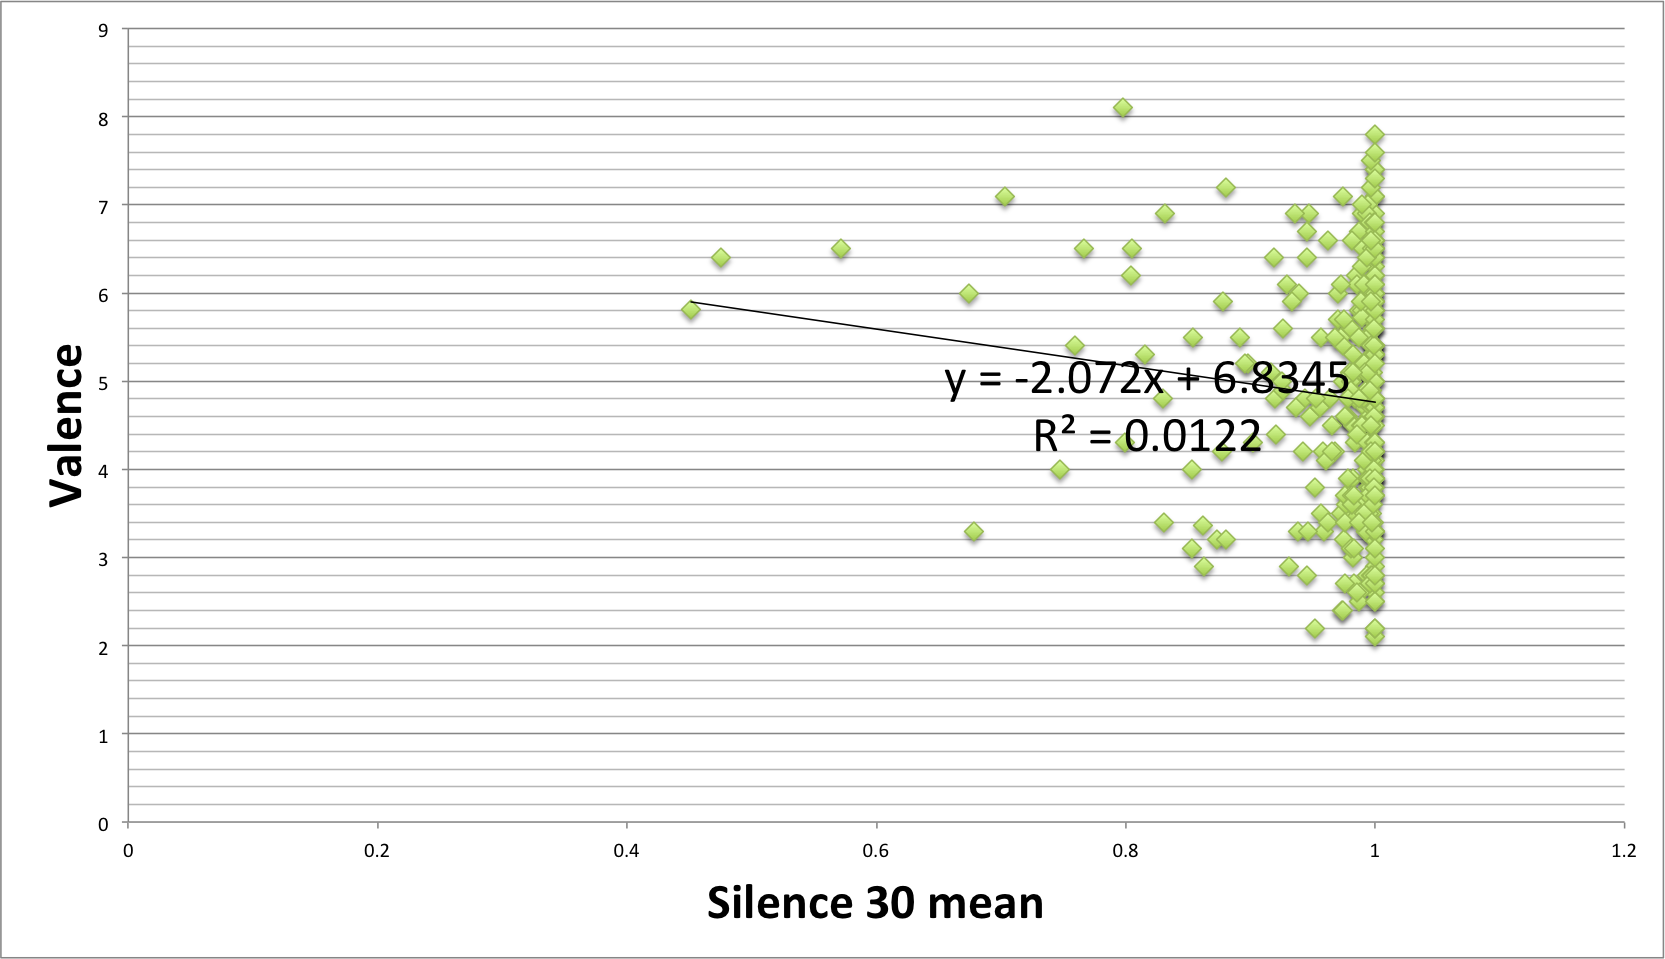
\includegraphics[width=\textwidth]{Figures/silence30mean-valence}
                  \vspace{20pt}
        \end{subfigure}
        
	    \centering
        \begin{subfigure}[b]{0.48\textwidth}
                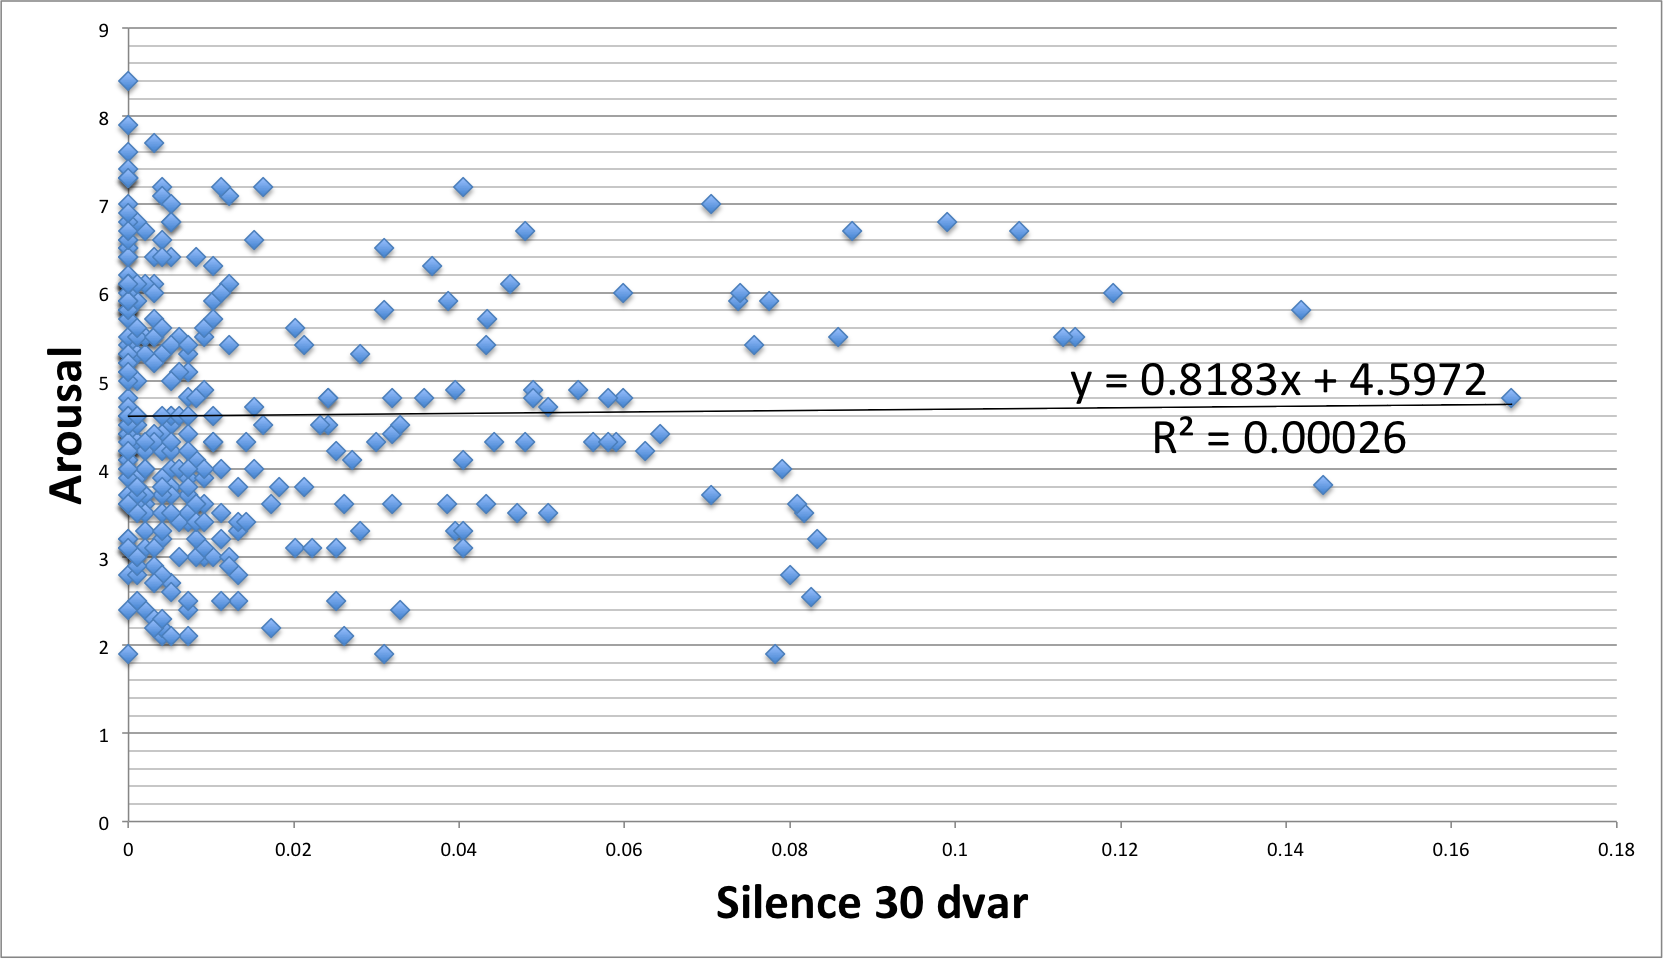
\includegraphics[width=\textwidth]{Figures/silence30dvar-arousal}
			   \vspace{20pt}
        \end{subfigure}
        \begin{subfigure}[b]{0.48\textwidth}
                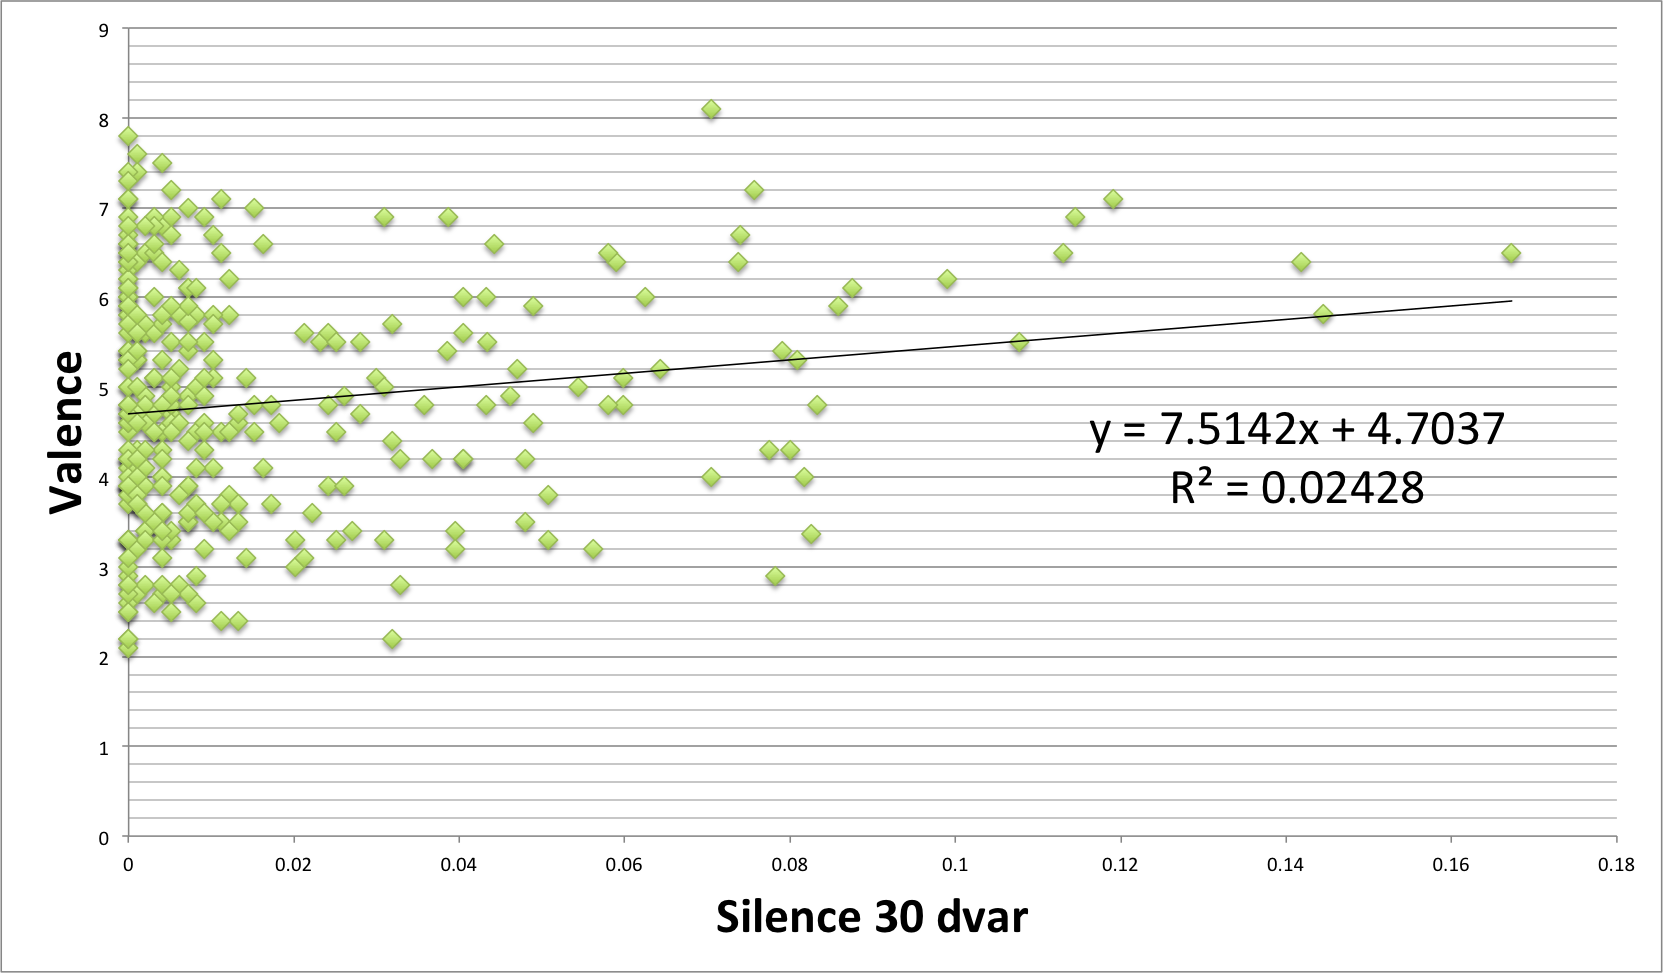
\includegraphics[width=\textwidth]{Figures/silence30dvar-valence}
                  \vspace{20pt}
        \end{subfigure}        
        
         \centering
        \begin{subfigure}[b]{0.48\textwidth}
                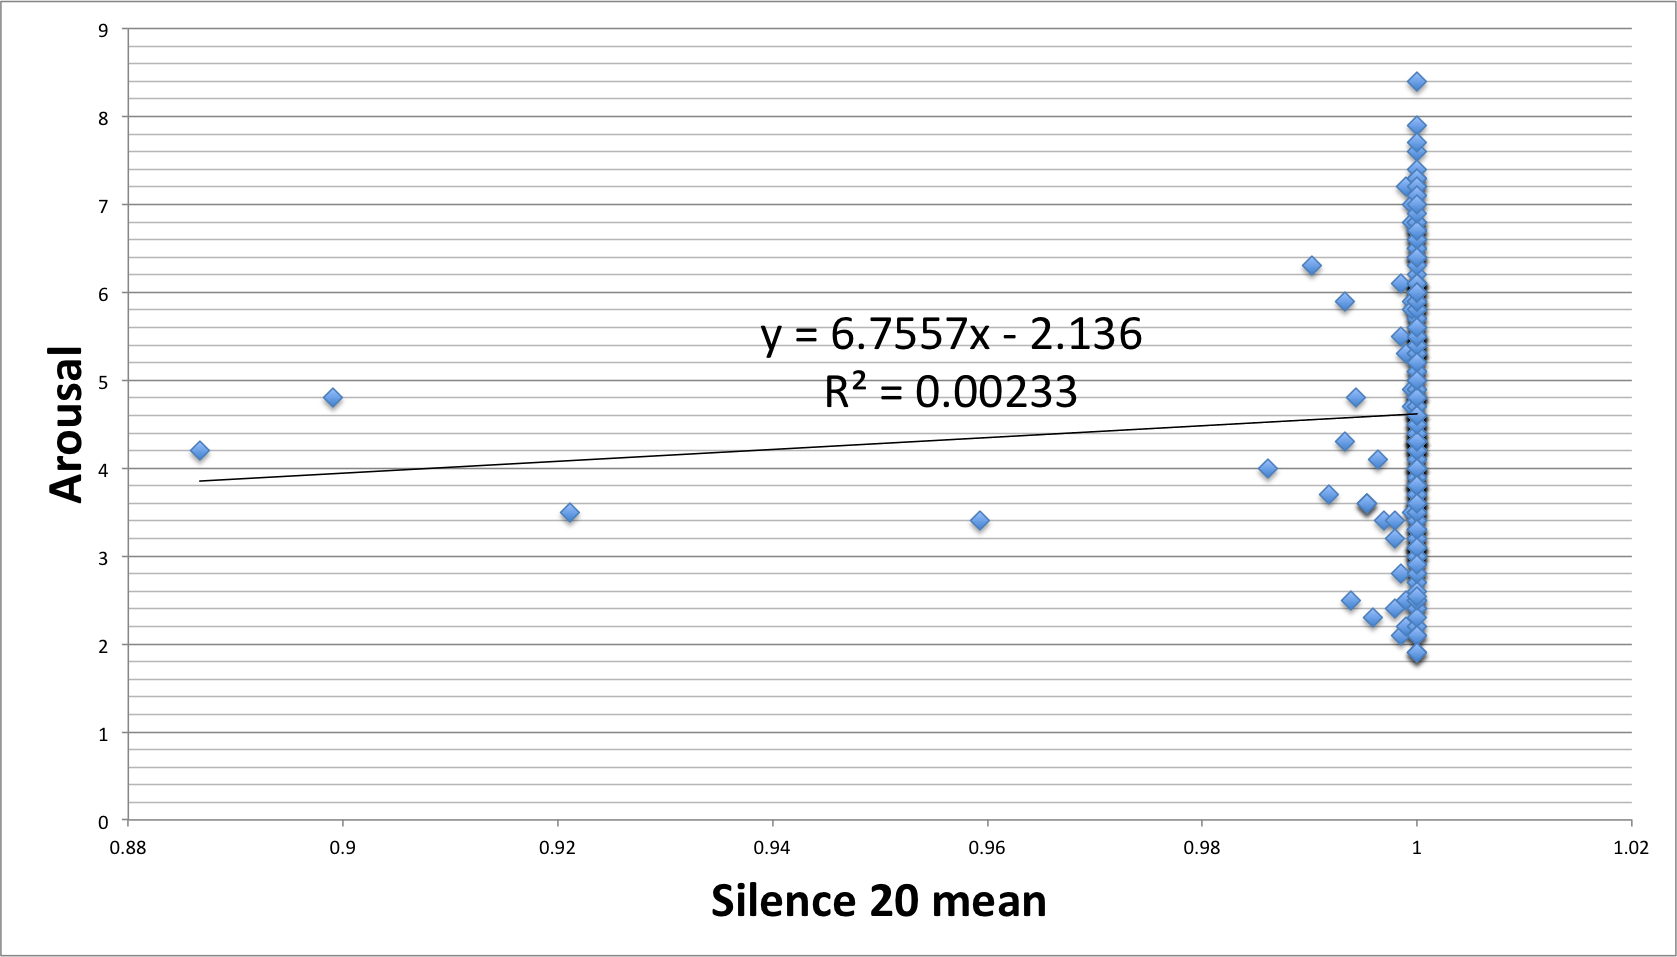
\includegraphics[width=\textwidth]{Figures/silence20mean-arousal}
			   \vspace{20pt}
        \end{subfigure}
        \begin{subfigure}[b]{0.48\textwidth}
                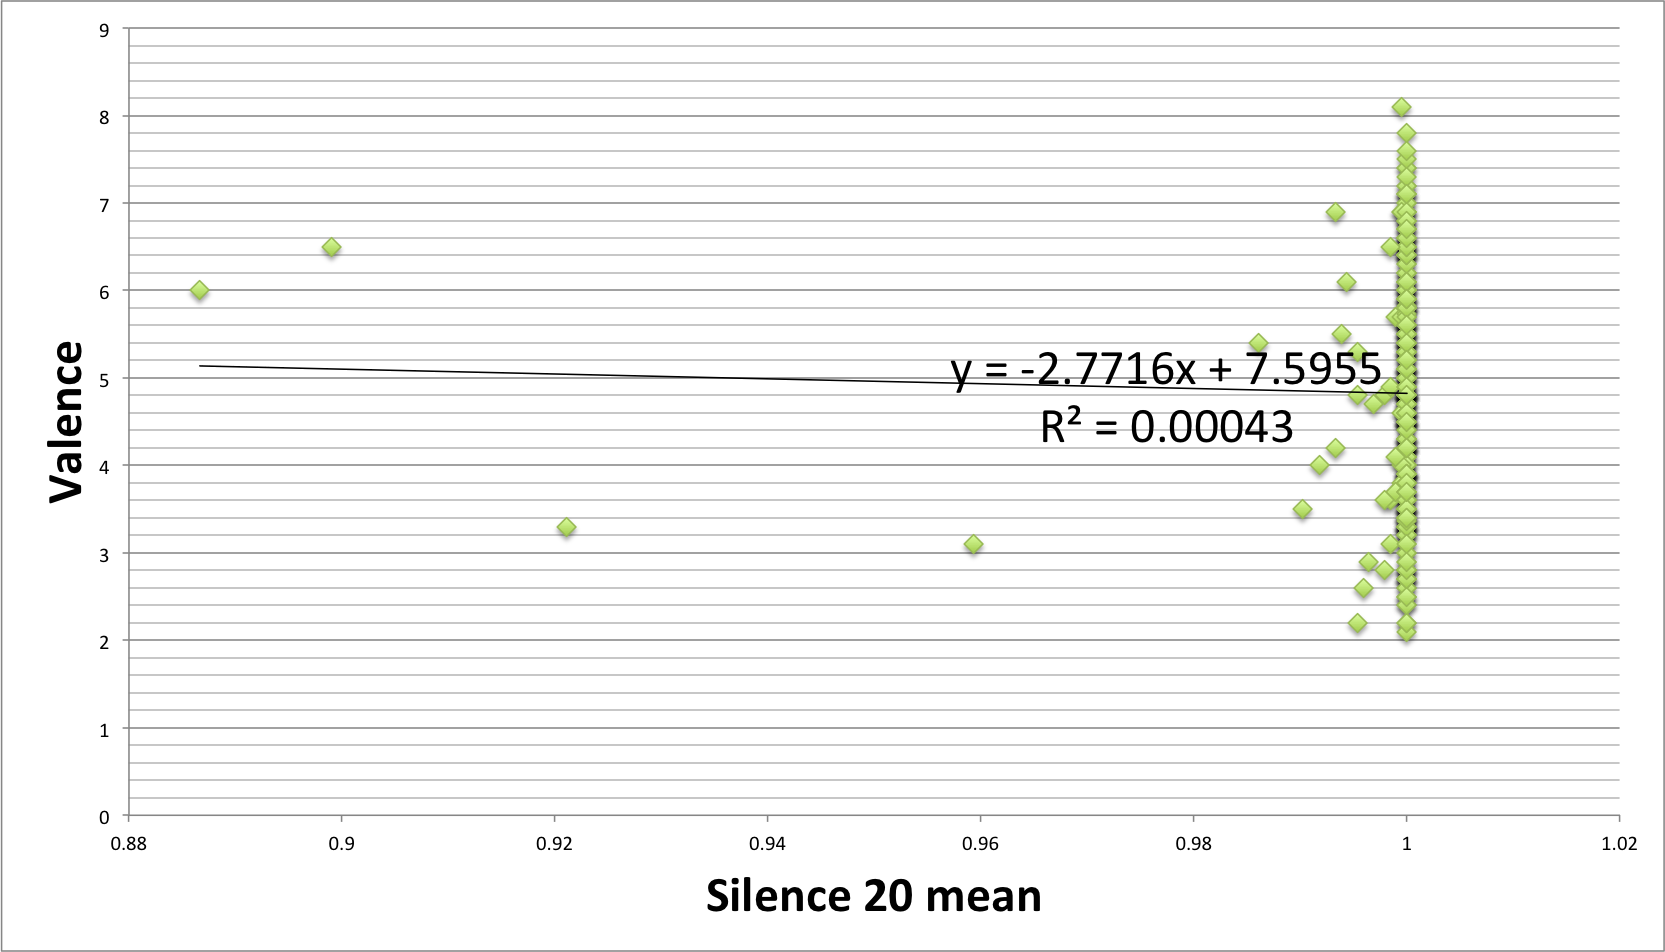
\includegraphics[width=\textwidth]{Figures/silence20mean-valence}
                  \vspace{20pt}
        \end{subfigure}
        
             \begin{subfigure}[b]{0.48\textwidth}
                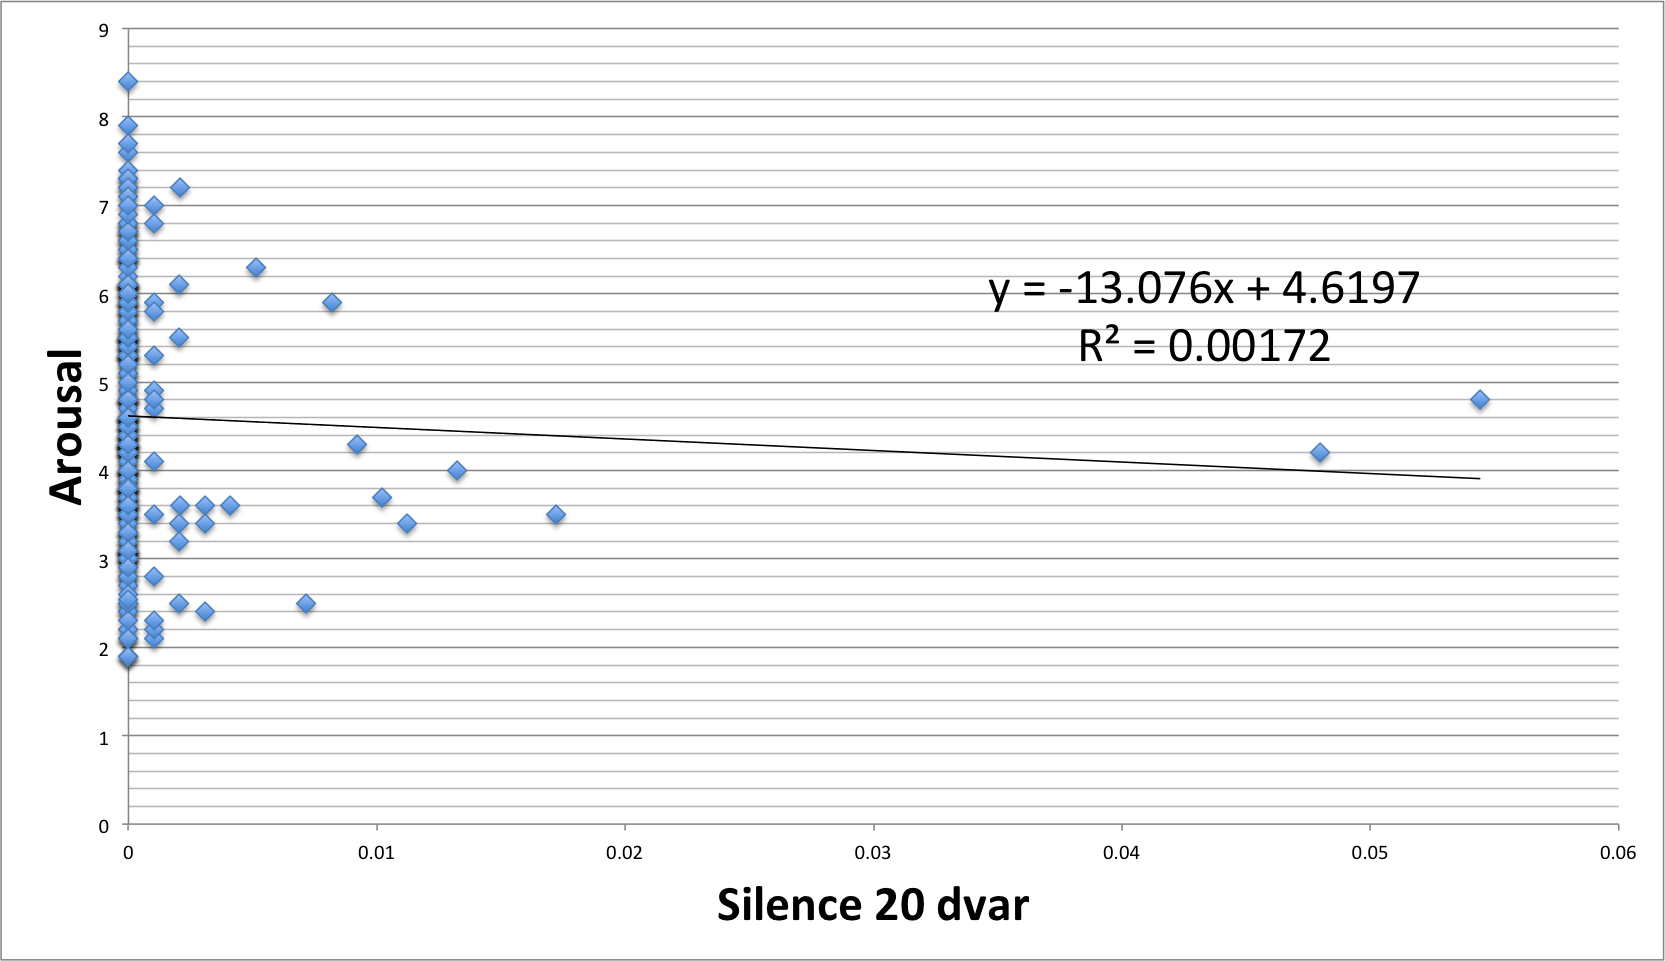
\includegraphics[width=\textwidth]{Figures/silence20dvar-arousal}
			   \vspace{20pt}
        \end{subfigure}
        \begin{subfigure}[b]{0.48\textwidth}
                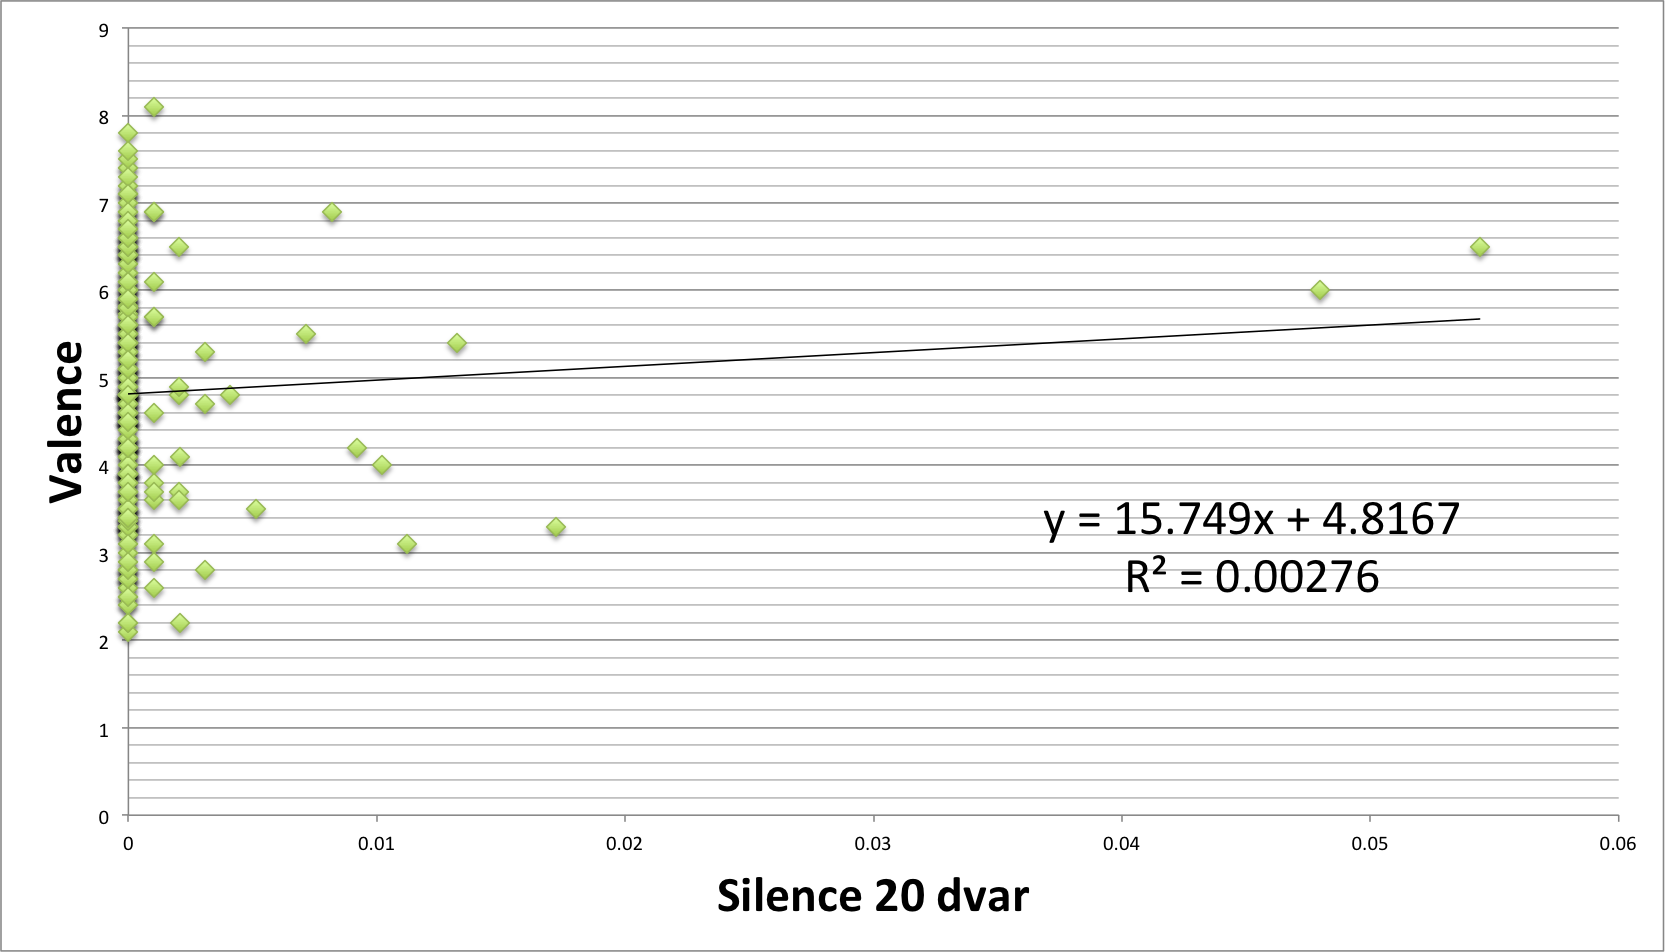
\includegraphics[width=\textwidth]{Figures/silence20dvar-valence}
                  \vspace{20pt}
        \end{subfigure}
        
\end{figure}

\begin{figure}
         \centering
        \begin{subfigure}[b]{0.48\textwidth}
                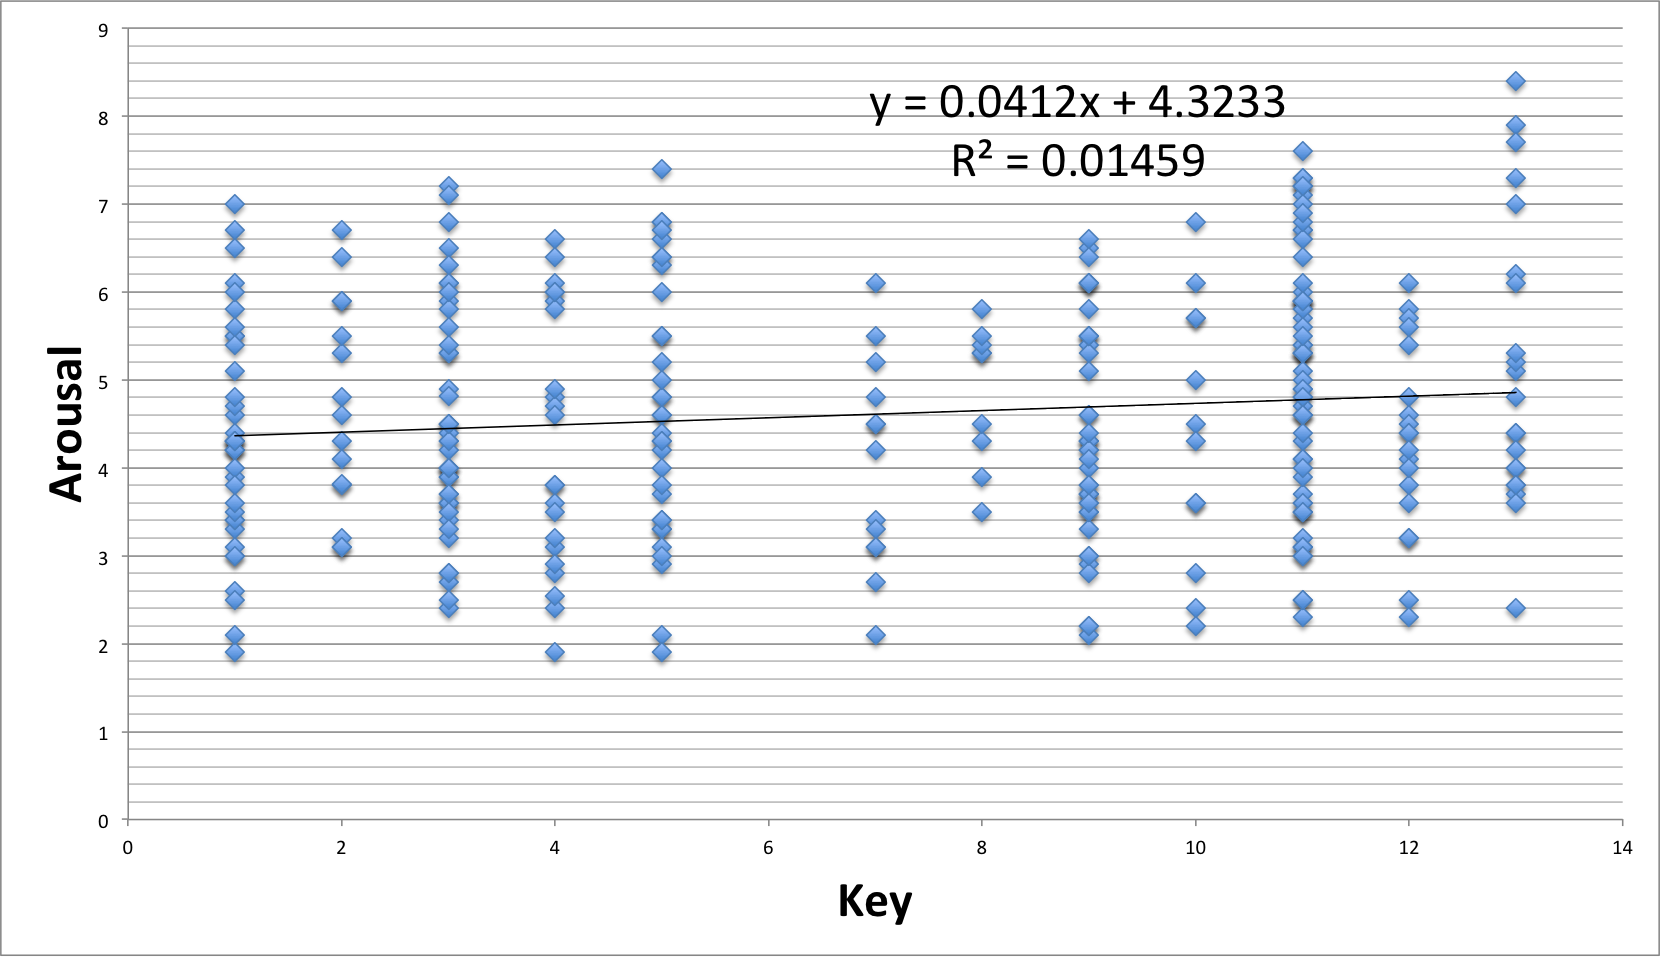
\includegraphics[width=\textwidth]{Figures/key-arousal}
			   \vspace{20pt}
        \end{subfigure}
        \begin{subfigure}[b]{0.48\textwidth}
                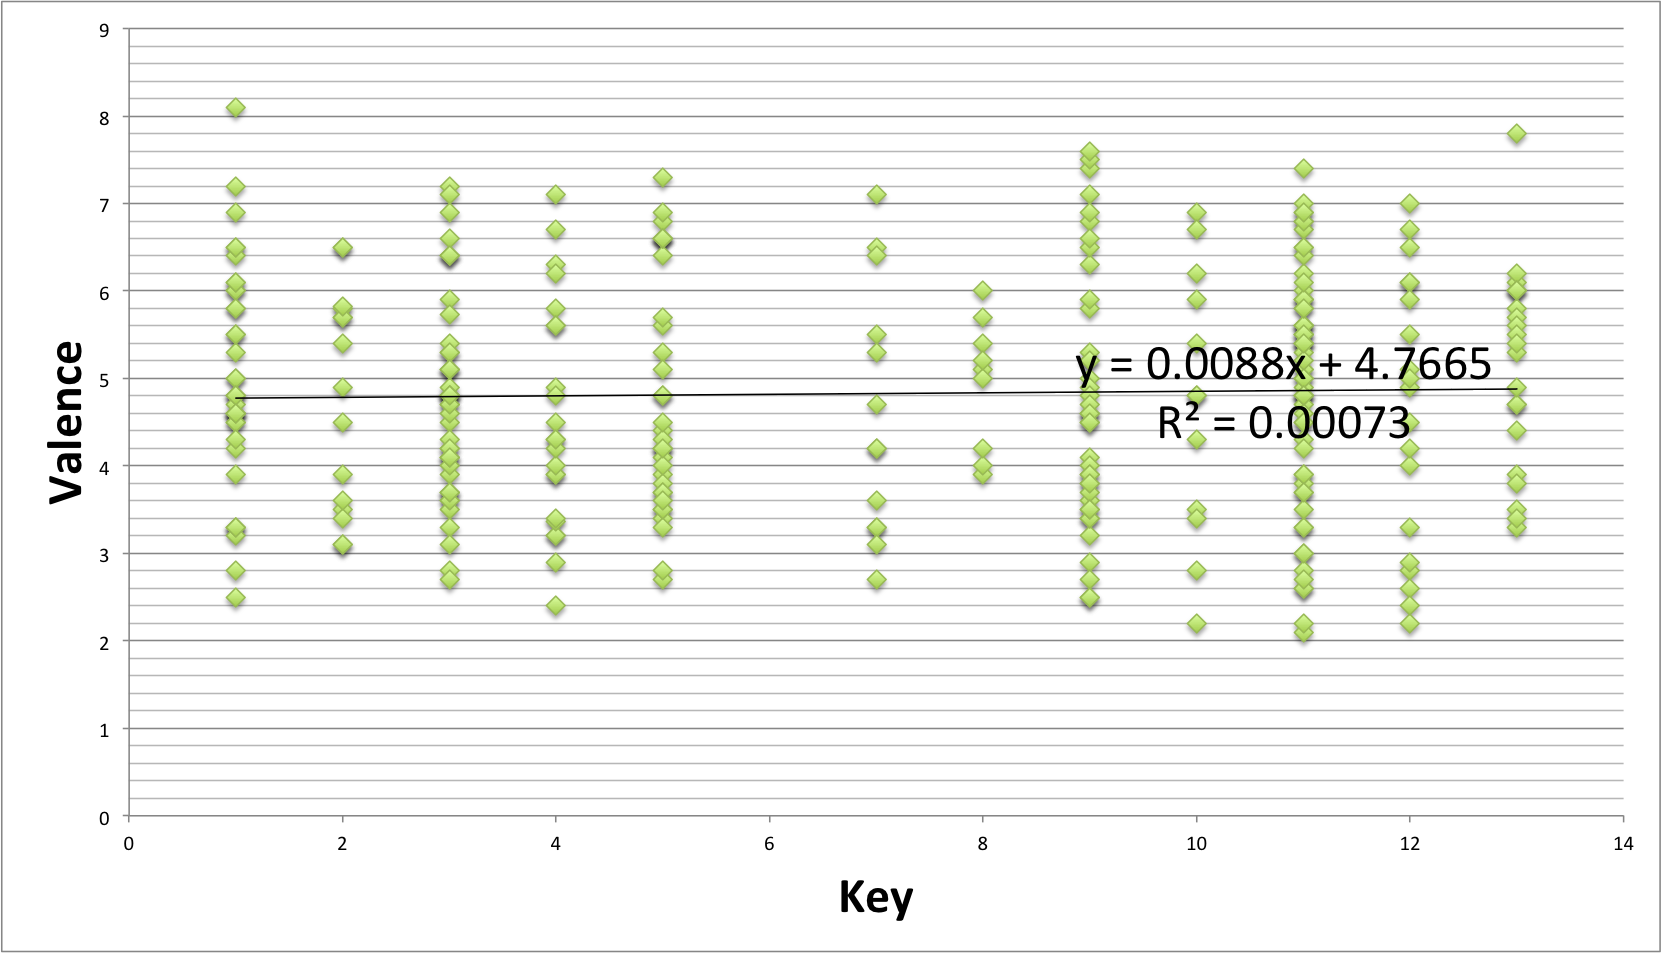
\includegraphics[width=\textwidth]{Figures/key-valence}
                  \vspace{20pt}
        \end{subfigure}
        
	    \centering
        \begin{subfigure}[b]{0.48\textwidth}
                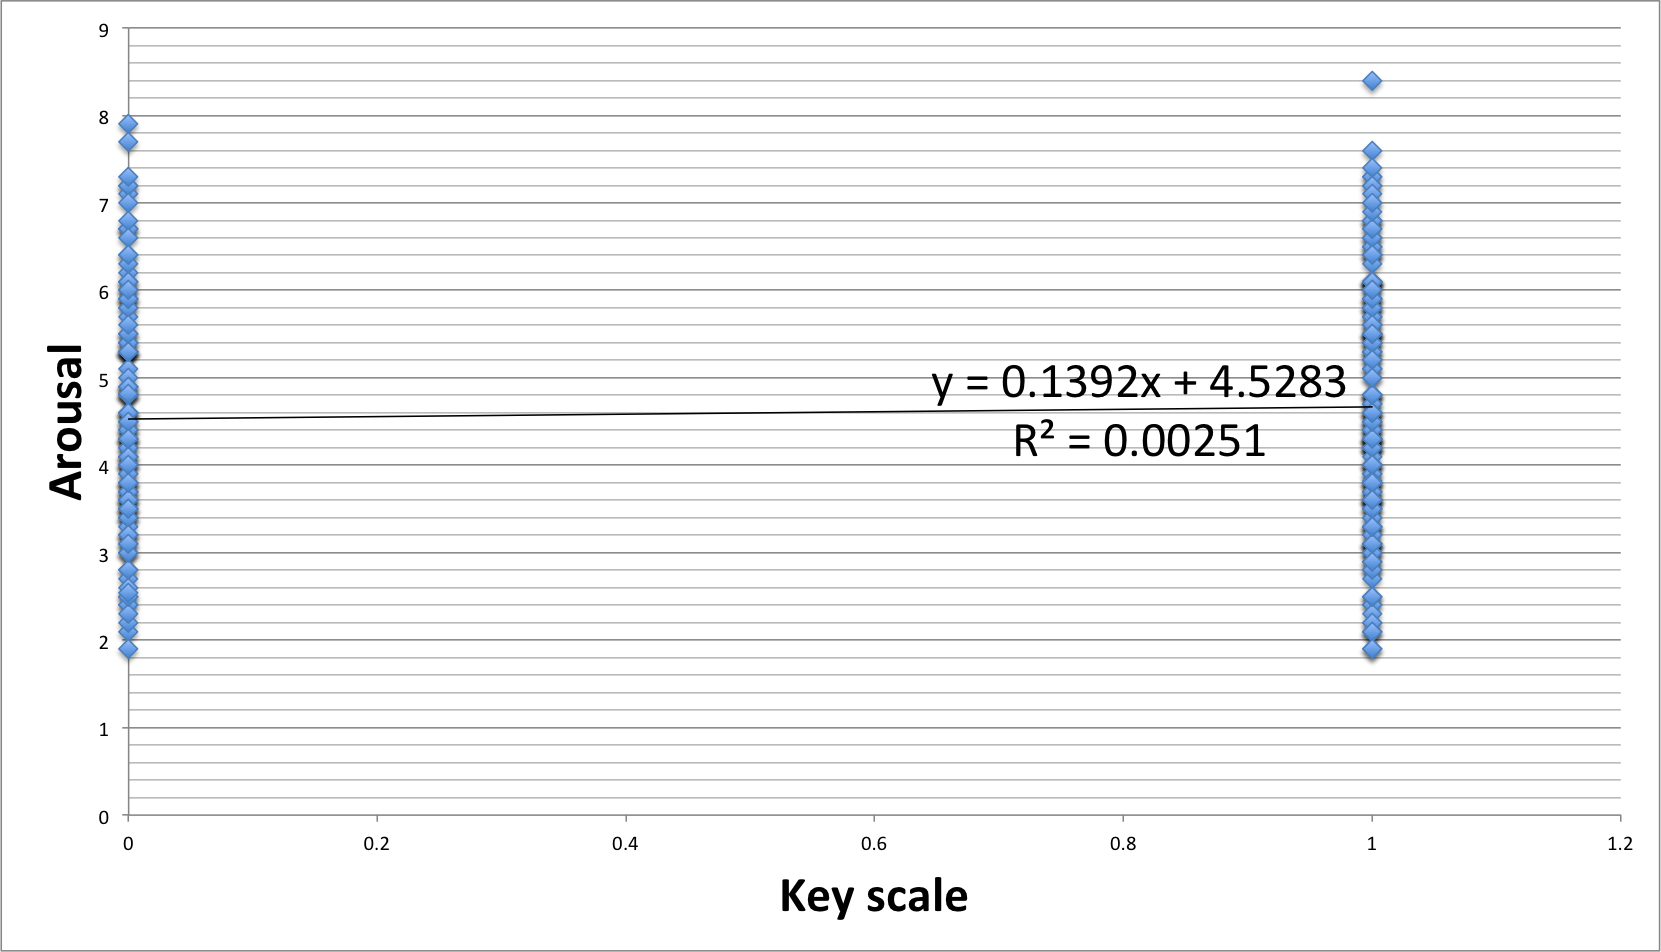
\includegraphics[width=\textwidth]{Figures/keyscale-arousal}
			   \vspace{20pt}
        \end{subfigure}
        \begin{subfigure}[b]{0.48\textwidth}
                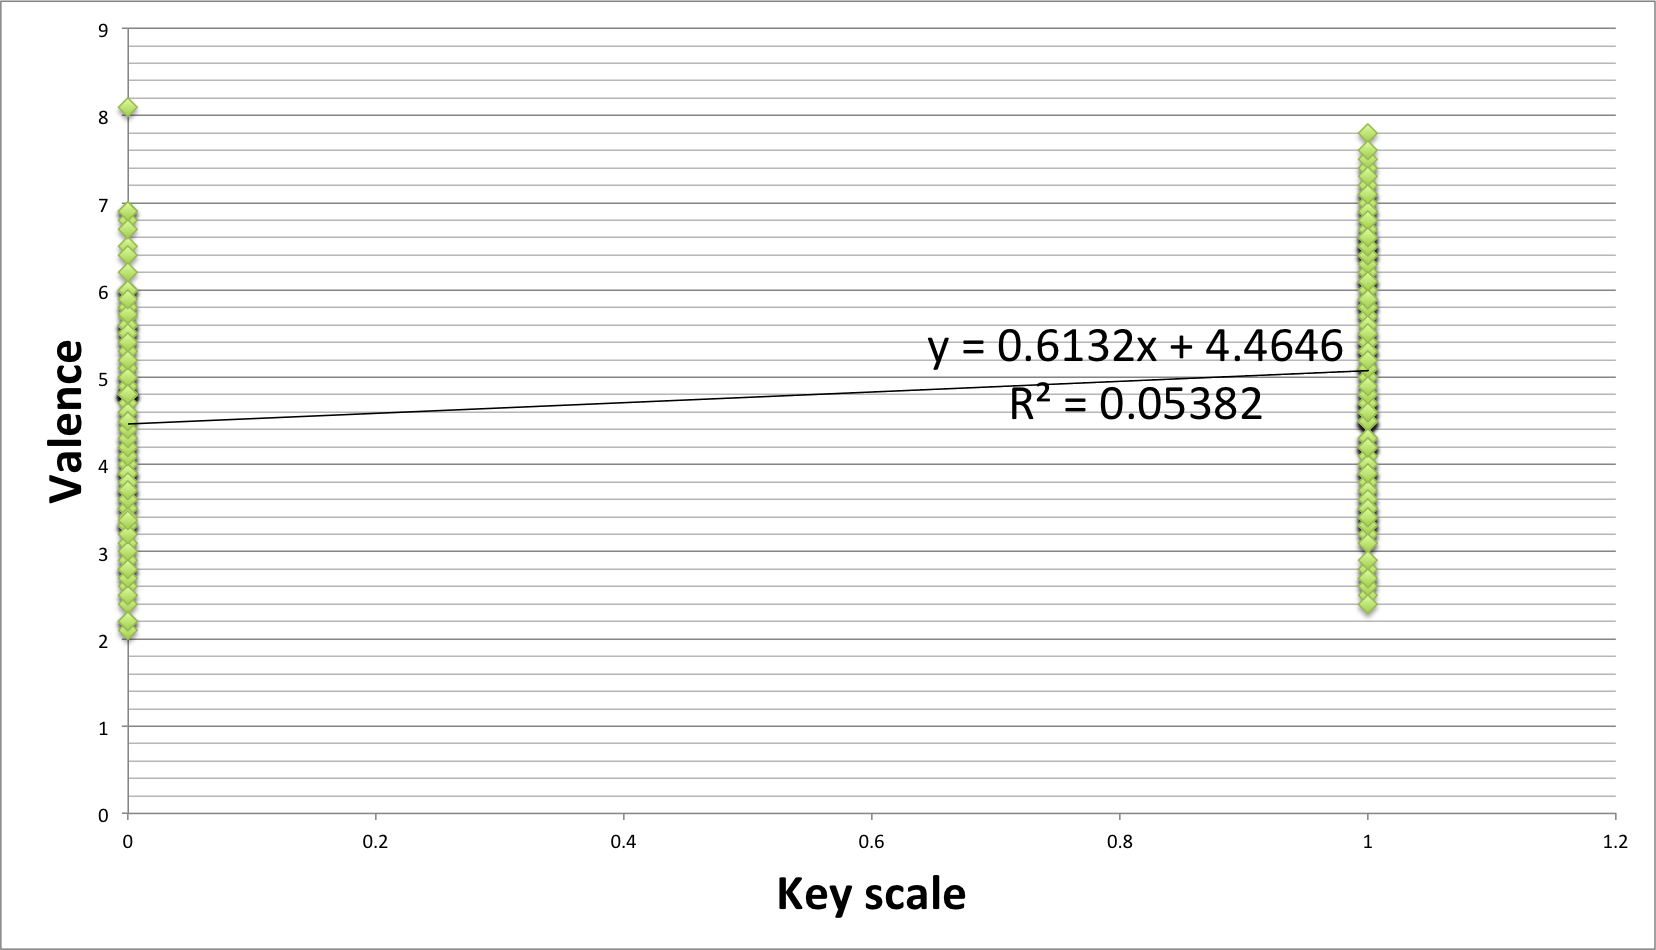
\includegraphics[width=\textwidth]{Figures/keyscale-valence}
                  \vspace{20pt}
        \end{subfigure}        
        
         \centering
        \begin{subfigure}[b]{0.48\textwidth}
                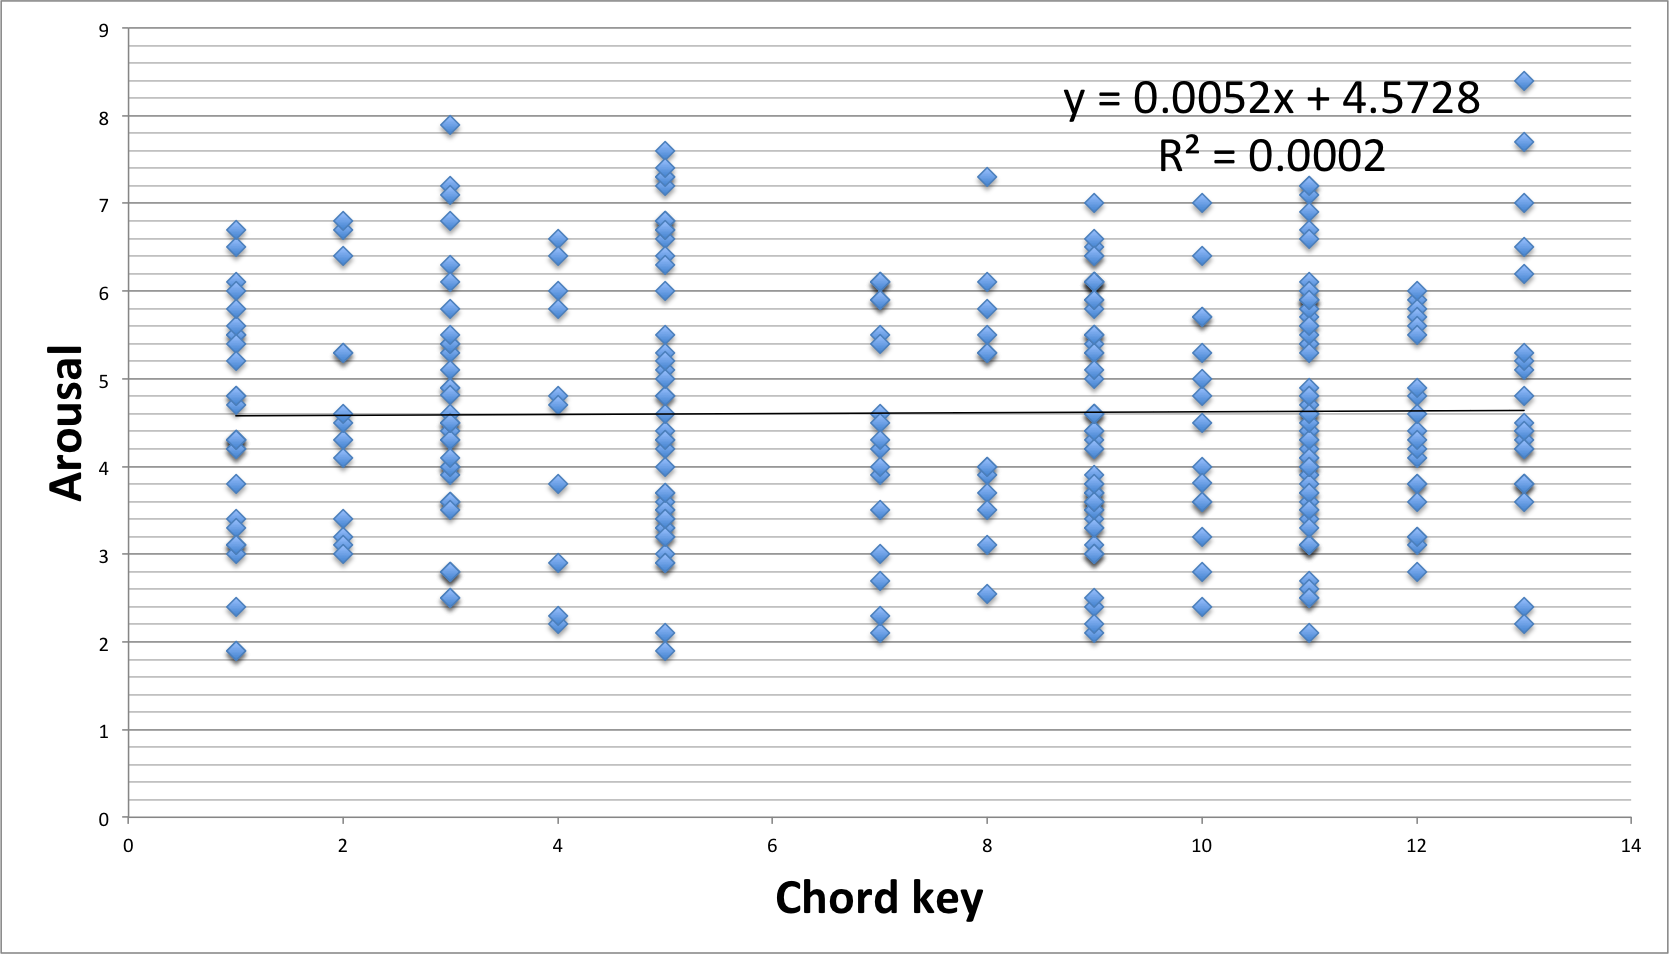
\includegraphics[width=\textwidth]{Figures/chordkey-arousal}
			   \vspace{20pt}
        \end{subfigure}
        \begin{subfigure}[b]{0.48\textwidth}
                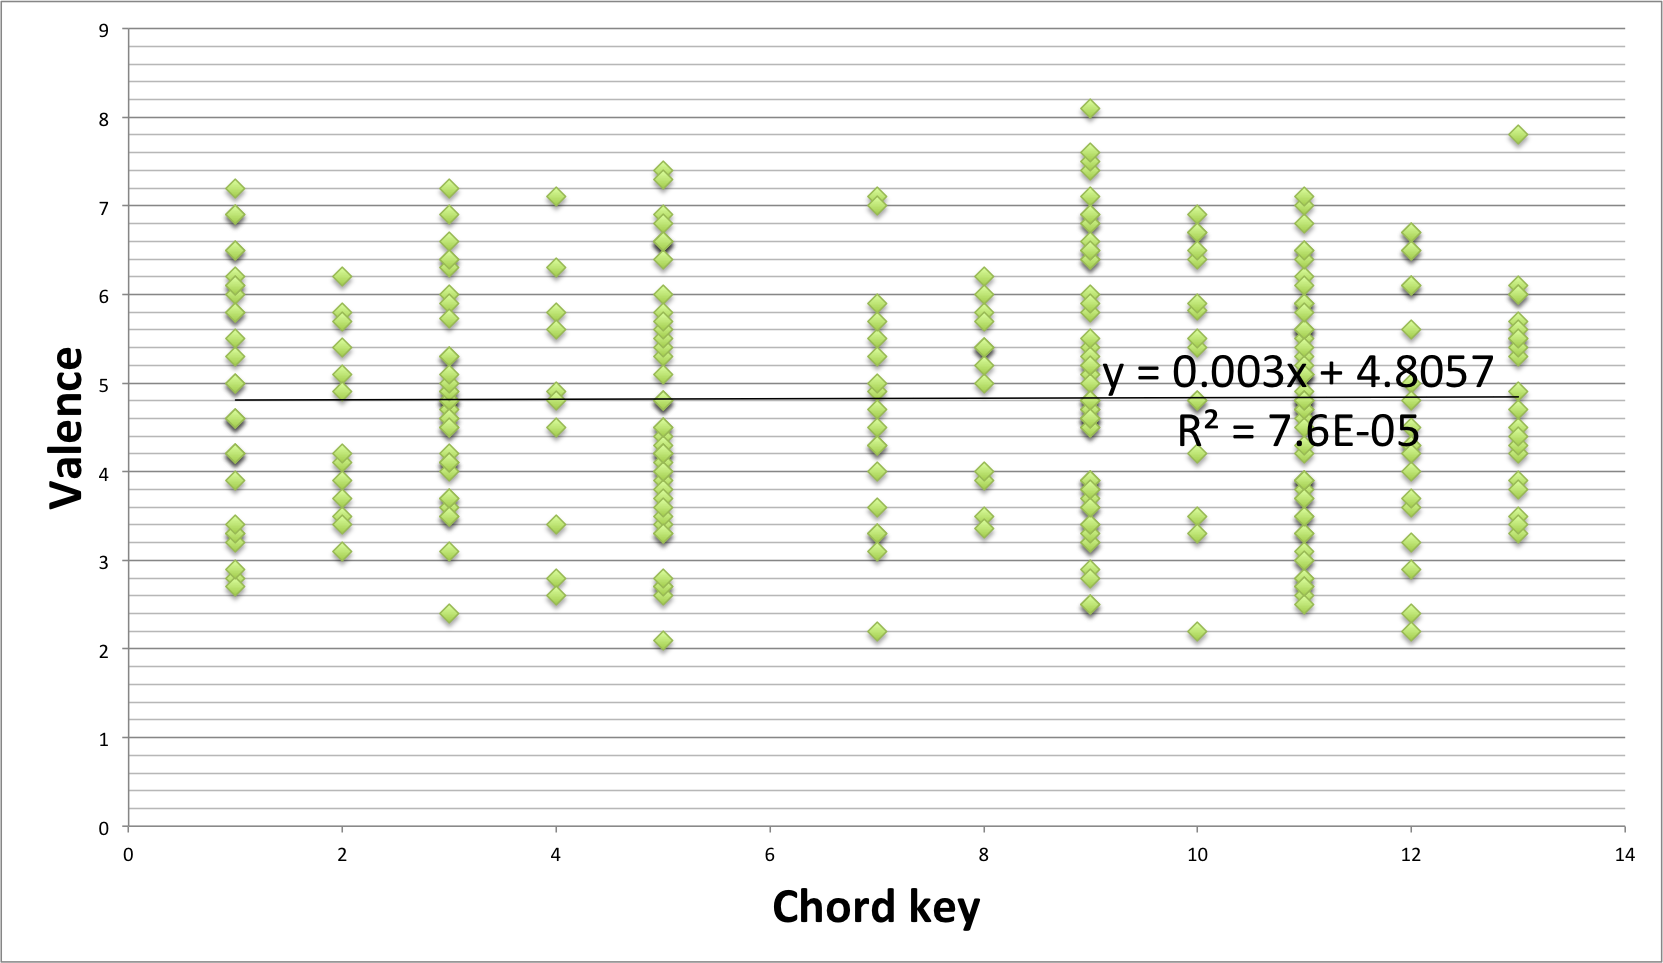
\includegraphics[width=\textwidth]{Figures/chordkey-valence}
                  \vspace{20pt}
        \end{subfigure}
        
             \begin{subfigure}[b]{0.48\textwidth}
                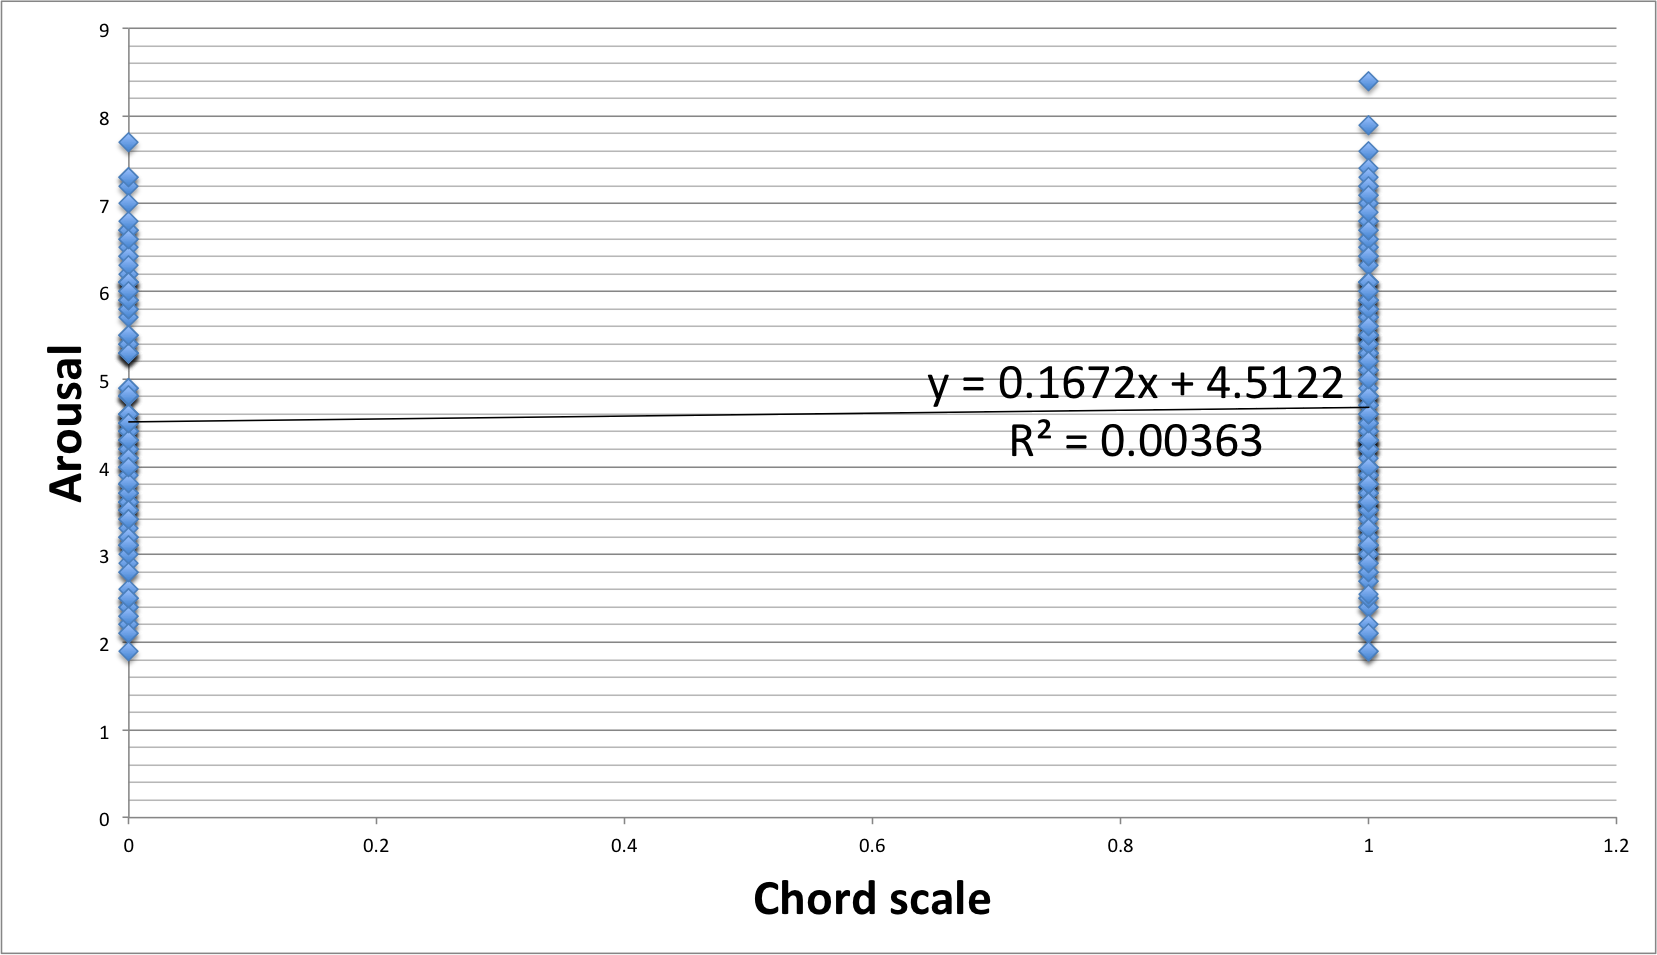
\includegraphics[width=\textwidth]{Figures/chordscale-arousal}
			   \vspace{20pt}
        \end{subfigure}
        \begin{subfigure}[b]{0.48\textwidth}
                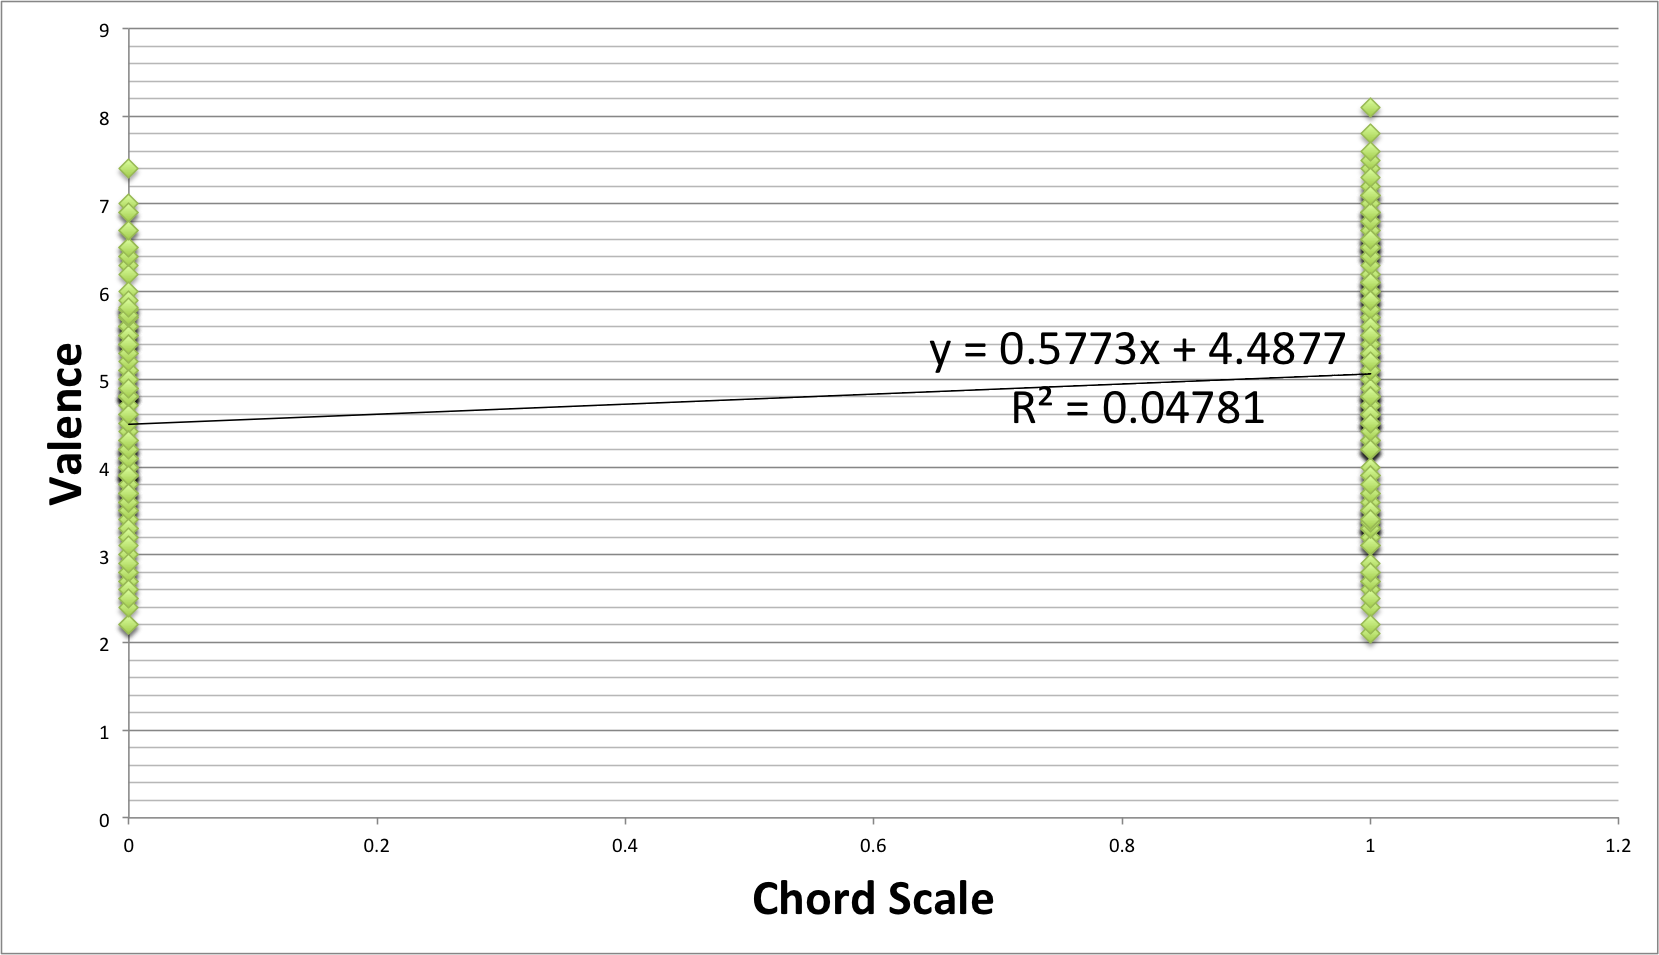
\includegraphics[width=\textwidth]{Figures/chordscale-valence}
                  \vspace{20pt}
        \end{subfigure}
        
\end{figure}

\begin{figure}
         \centering
        \begin{subfigure}[b]{0.48\textwidth}
                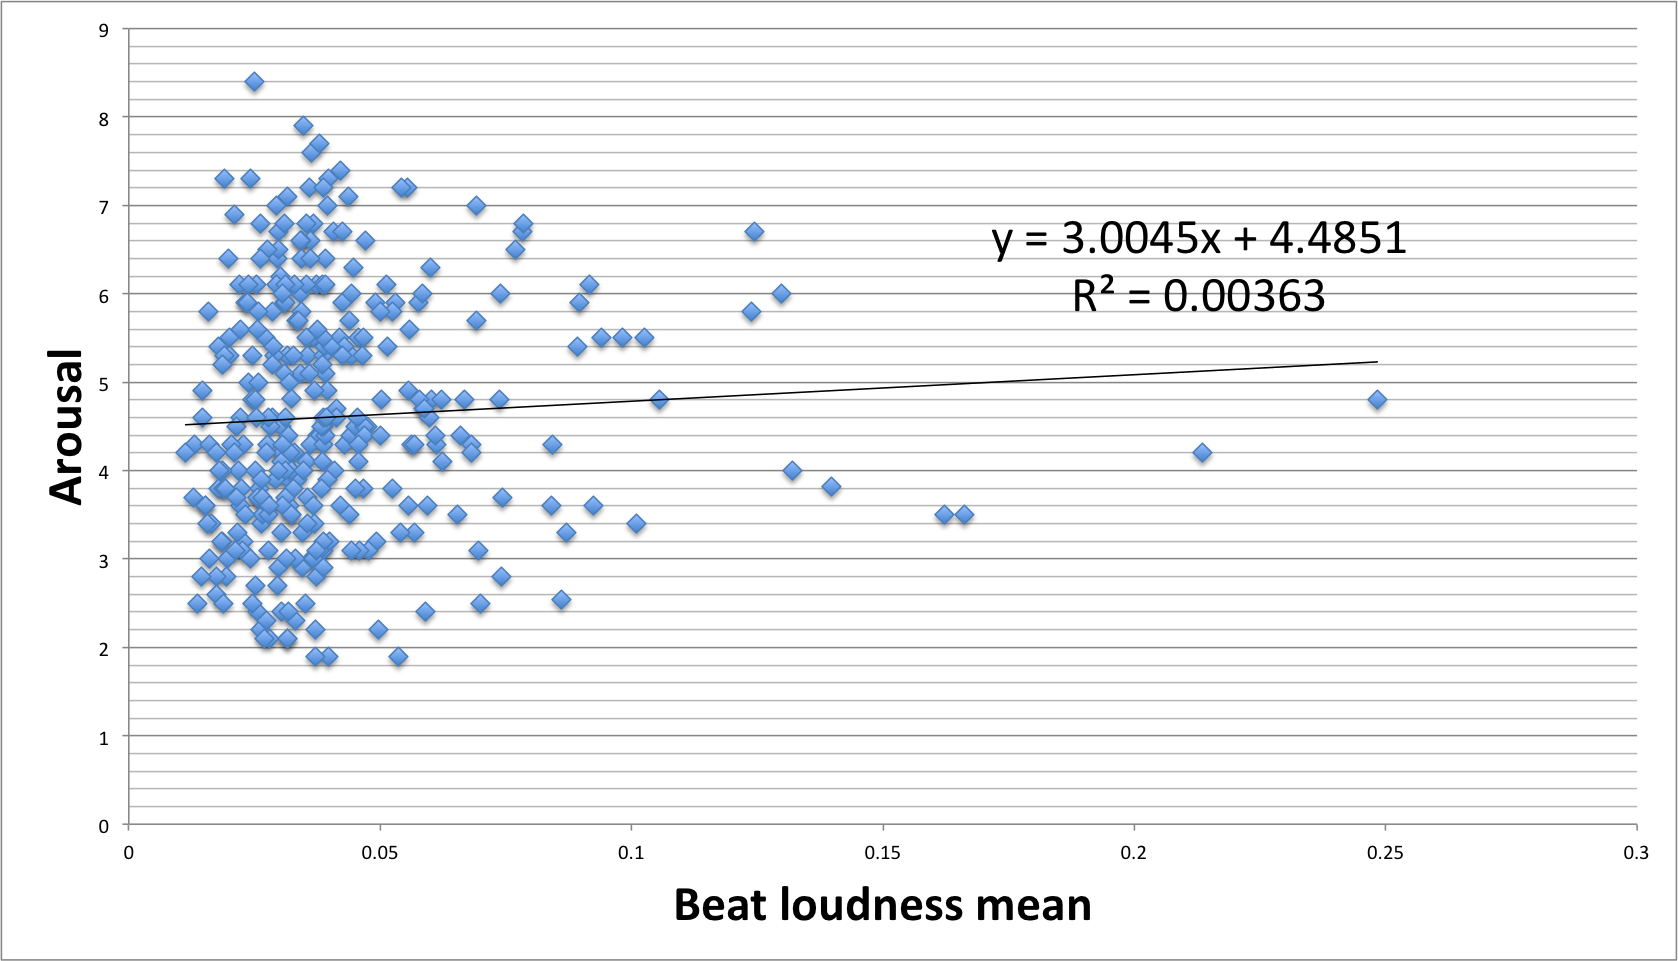
\includegraphics[width=\textwidth]{Figures/beatloudnessmean-arousal}
			   \vspace{20pt}
        \end{subfigure}
        \begin{subfigure}[b]{0.48\textwidth}
                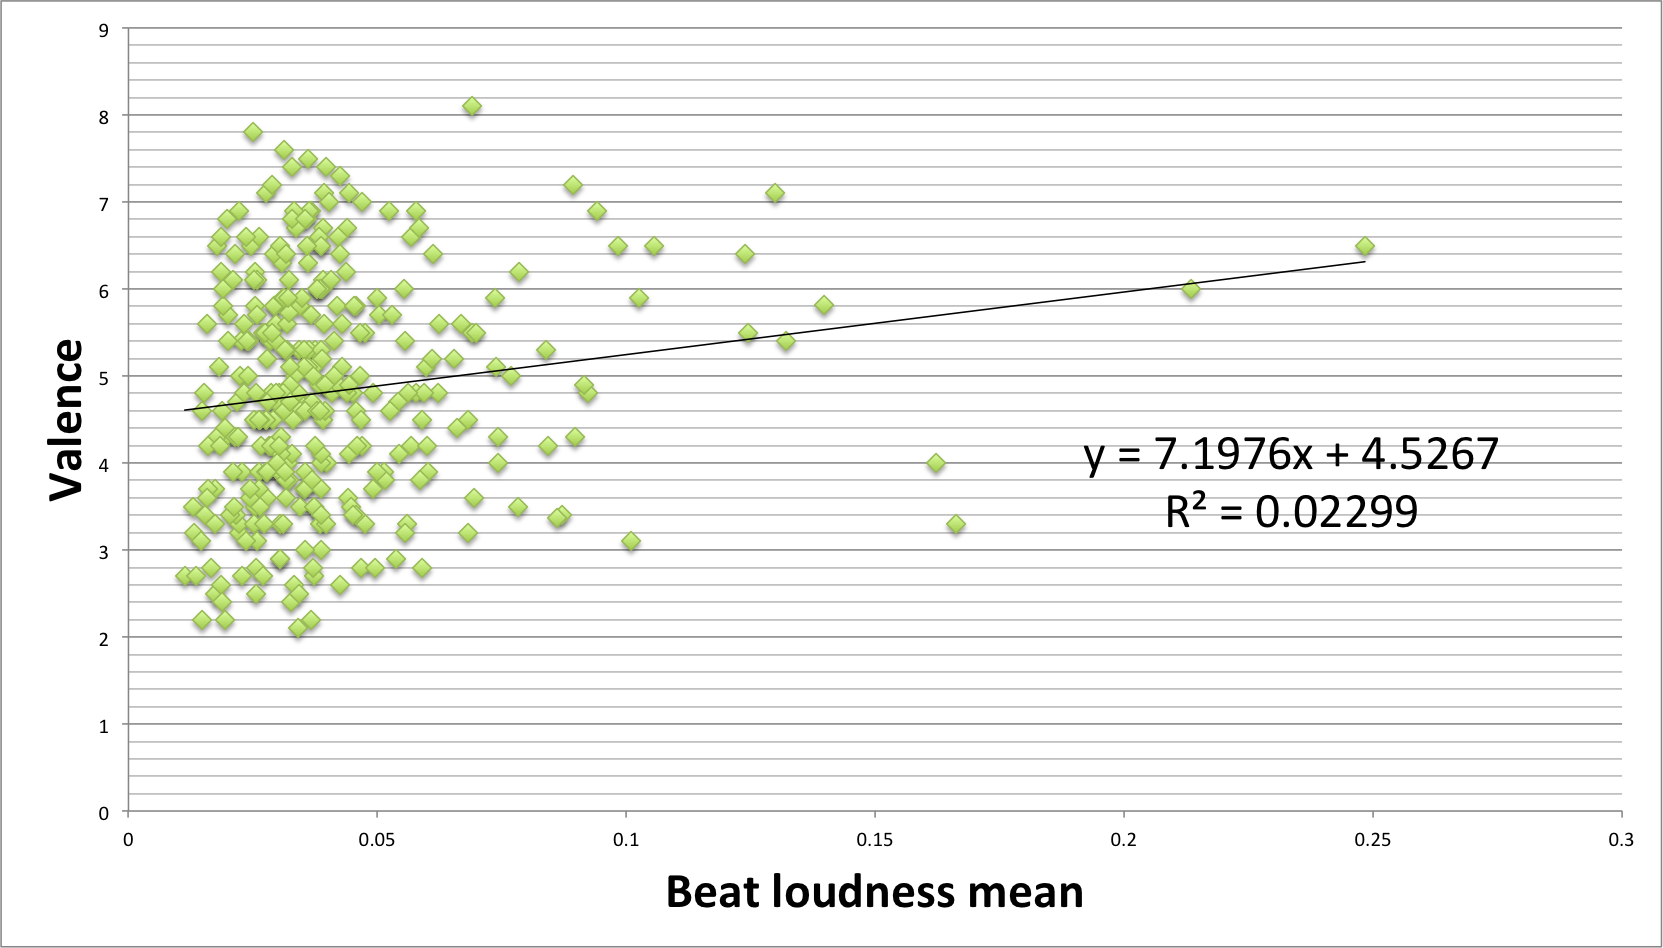
\includegraphics[width=\textwidth]{Figures/beatloudnessmean-valence}
                  \vspace{20pt}
        \end{subfigure}
        
	    \centering
        \begin{subfigure}[b]{0.48\textwidth}
                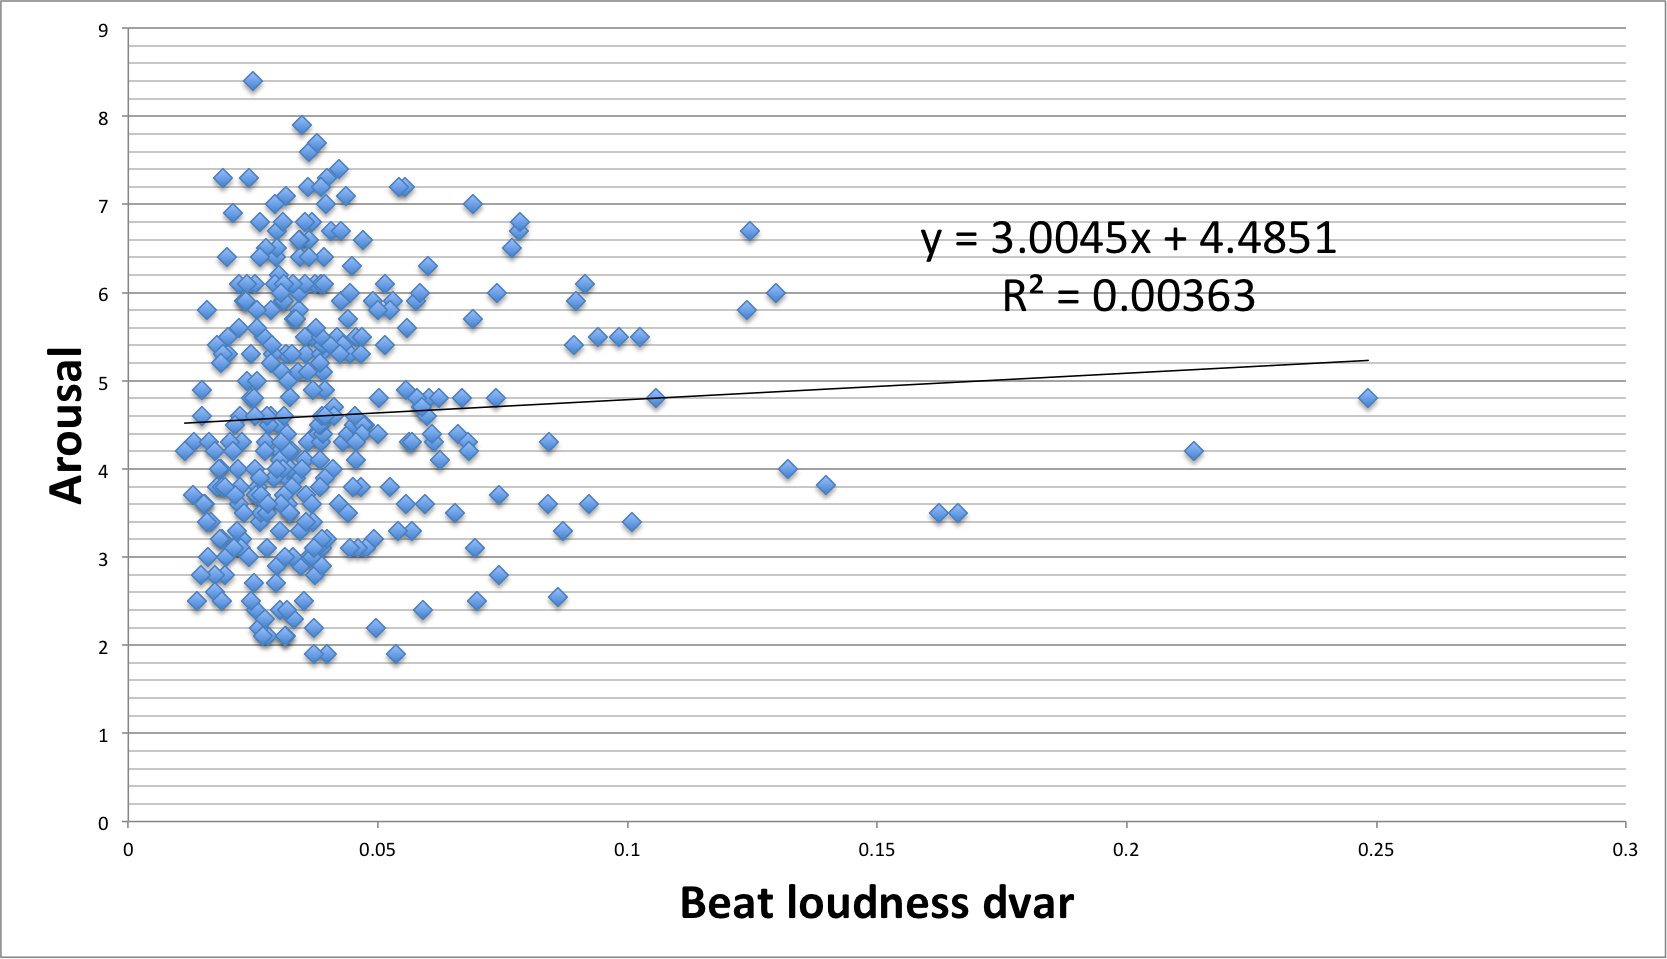
\includegraphics[width=\textwidth]{Figures/beatloudnessdvar-arousal}
			   \vspace{20pt}
        \end{subfigure}
        \begin{subfigure}[b]{0.48\textwidth}
                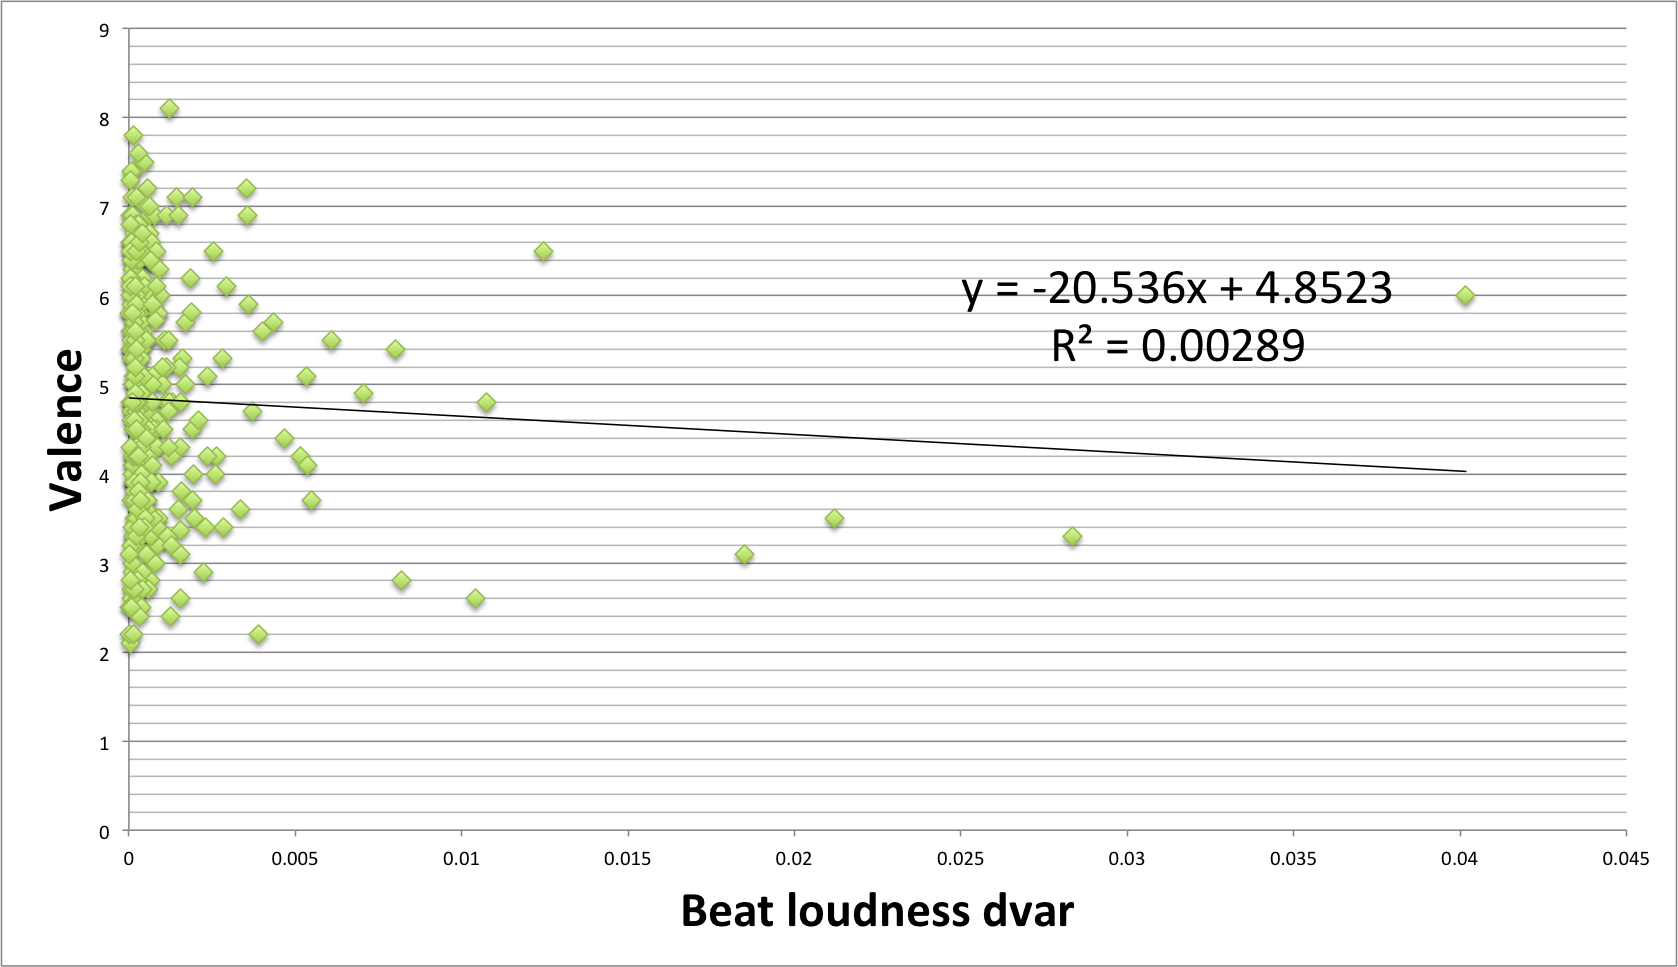
\includegraphics[width=\textwidth]{Figures/beatloudnessdvar-valence}
                  \vspace{20pt}
        \end{subfigure}        
        
         \centering
        \begin{subfigure}[b]{0.48\textwidth}
                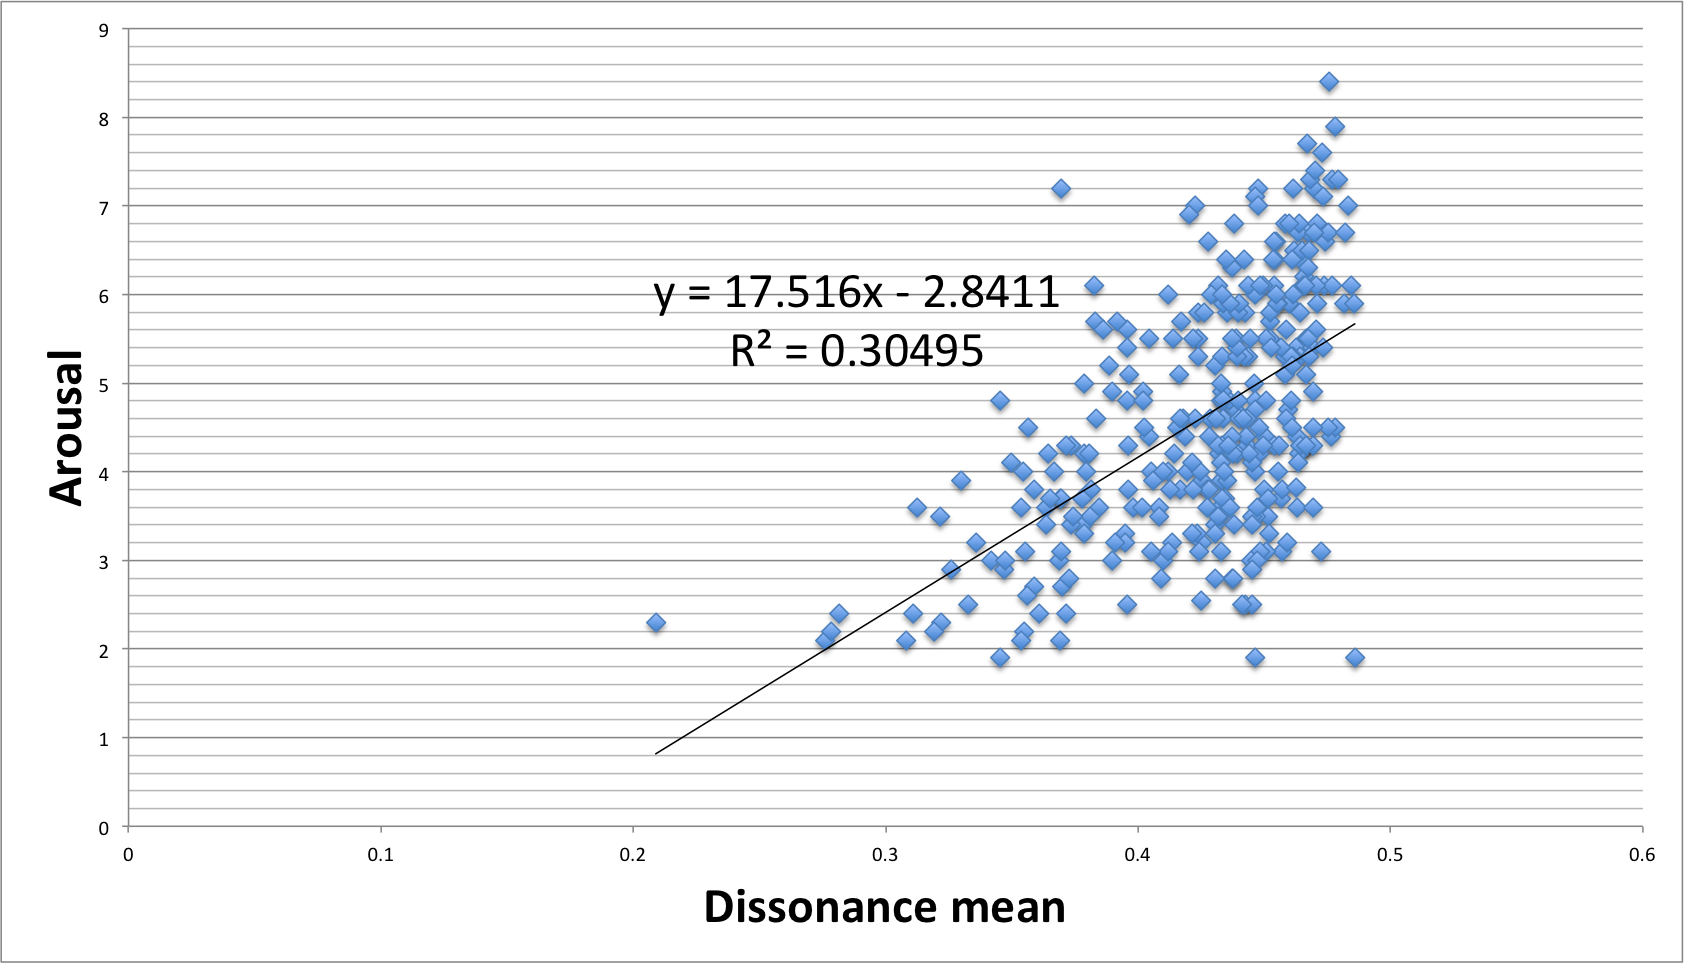
\includegraphics[width=\textwidth]{Figures/dissonancemean-arousal}
			   \vspace{20pt}
        \end{subfigure}
        \begin{subfigure}[b]{0.48\textwidth}
                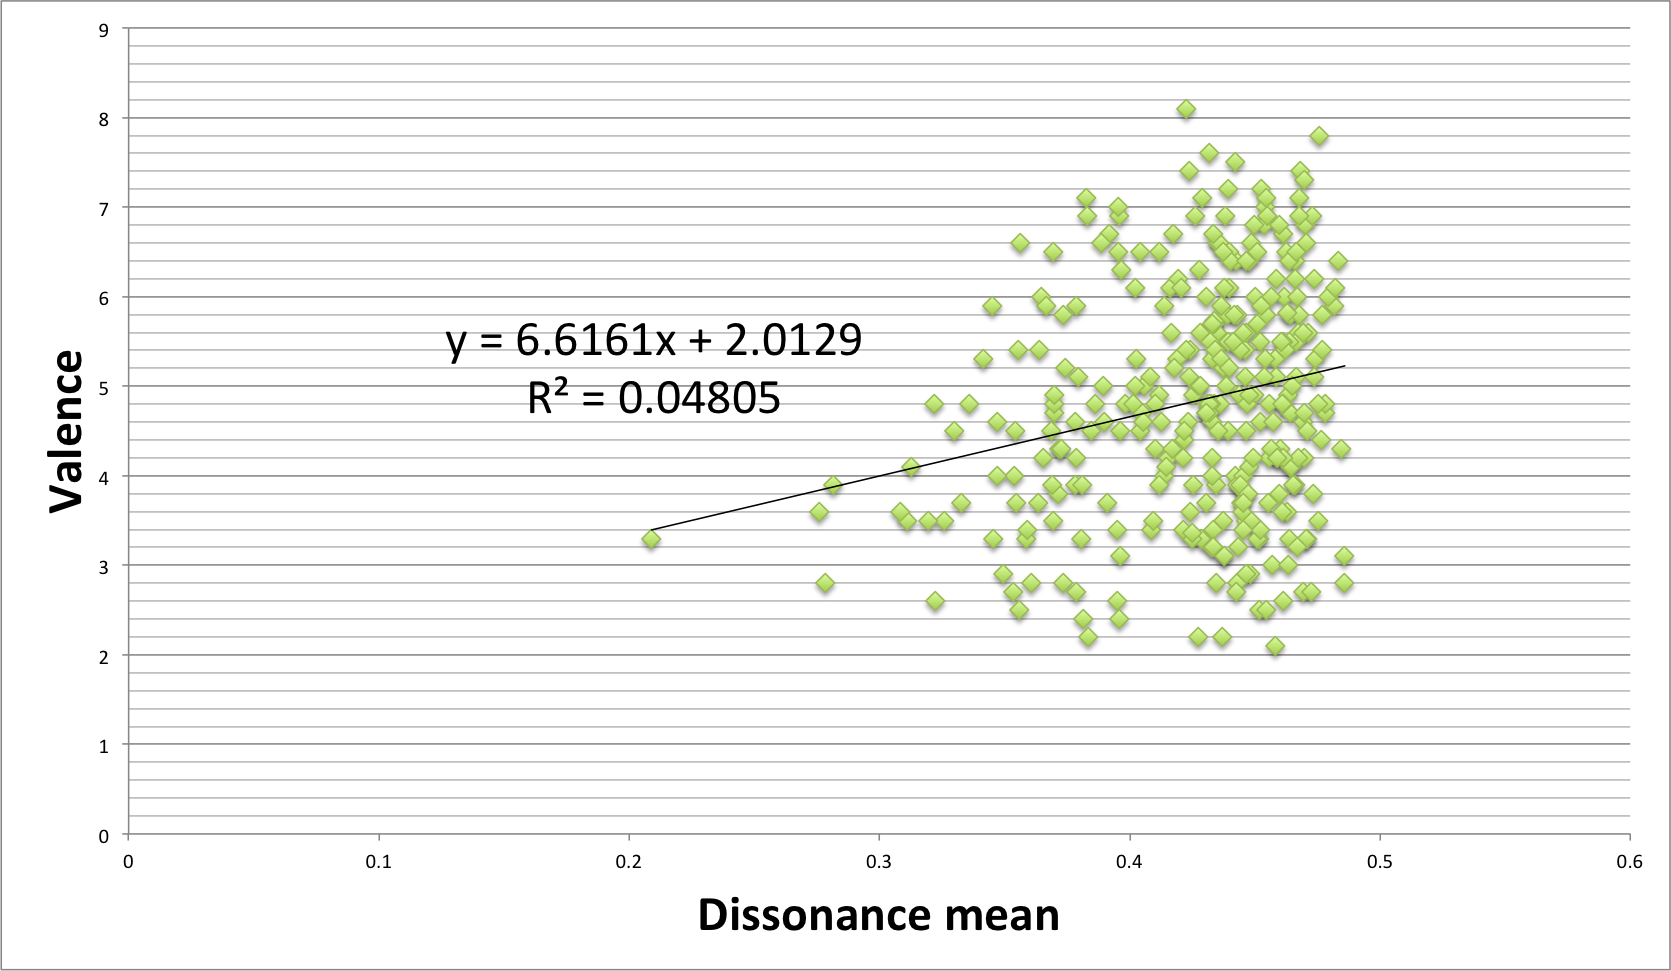
\includegraphics[width=\textwidth]{Figures/dissonancemean-valence}
                  \vspace{20pt}
        \end{subfigure}
        
	    \centering
        \begin{subfigure}[b]{0.48\textwidth}
                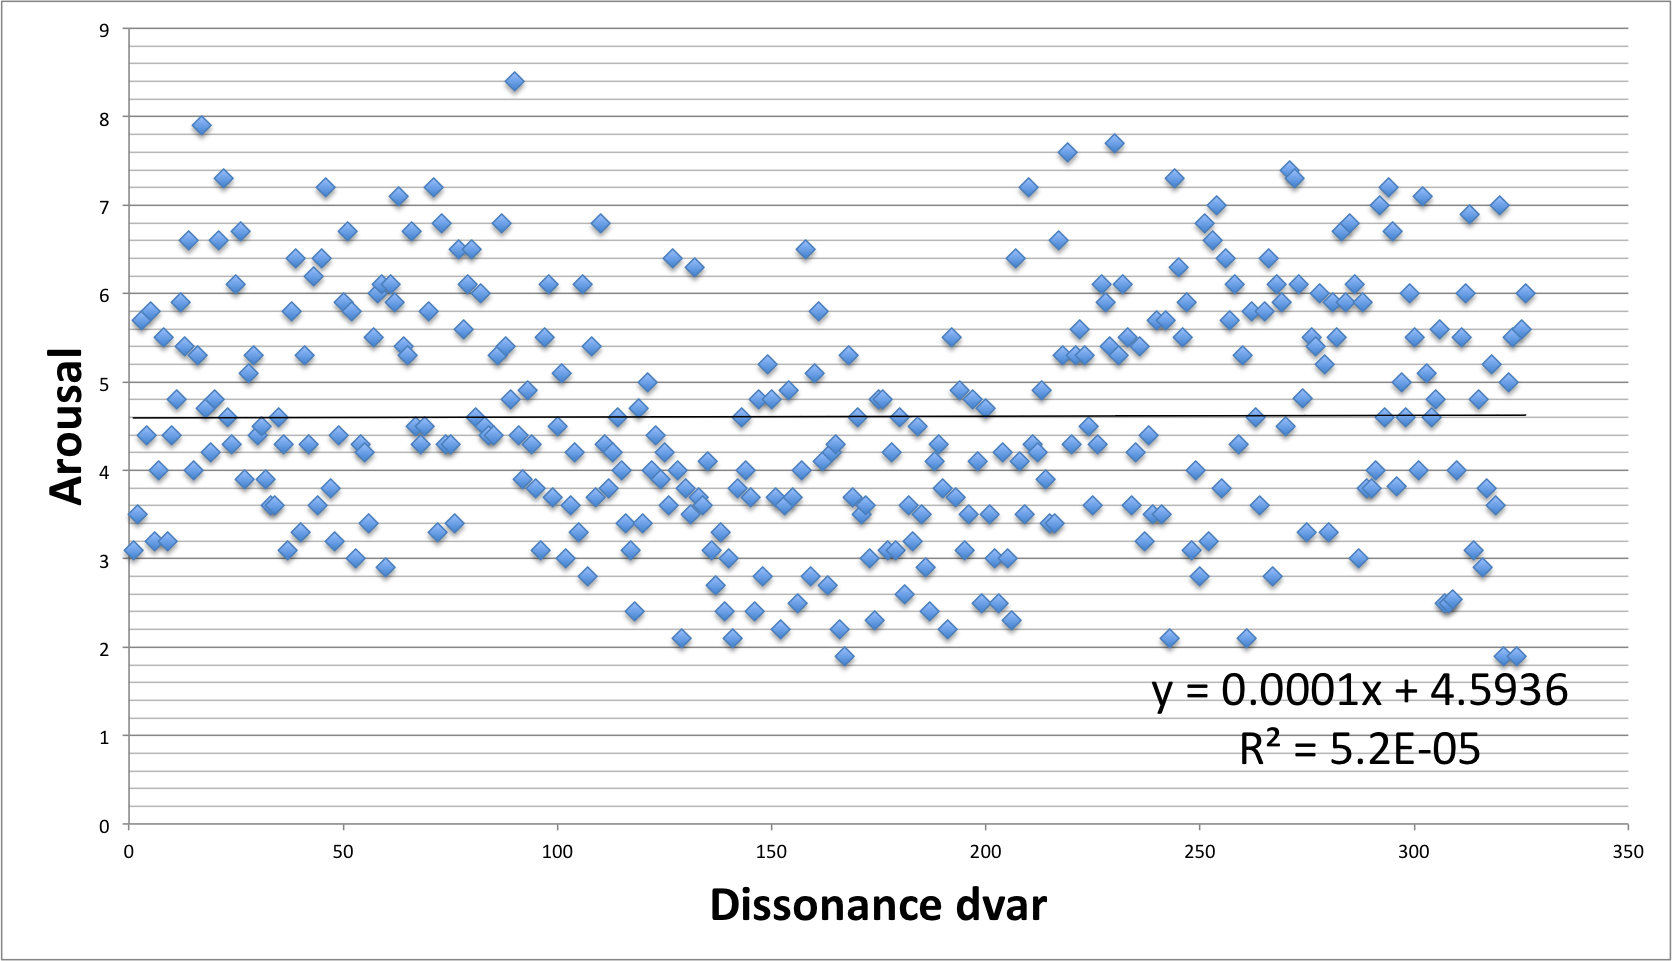
\includegraphics[width=\textwidth]{Figures/dissonancedvar-arousal}
			   \vspace{20pt}
        \end{subfigure}
        \begin{subfigure}[b]{0.48\textwidth}
                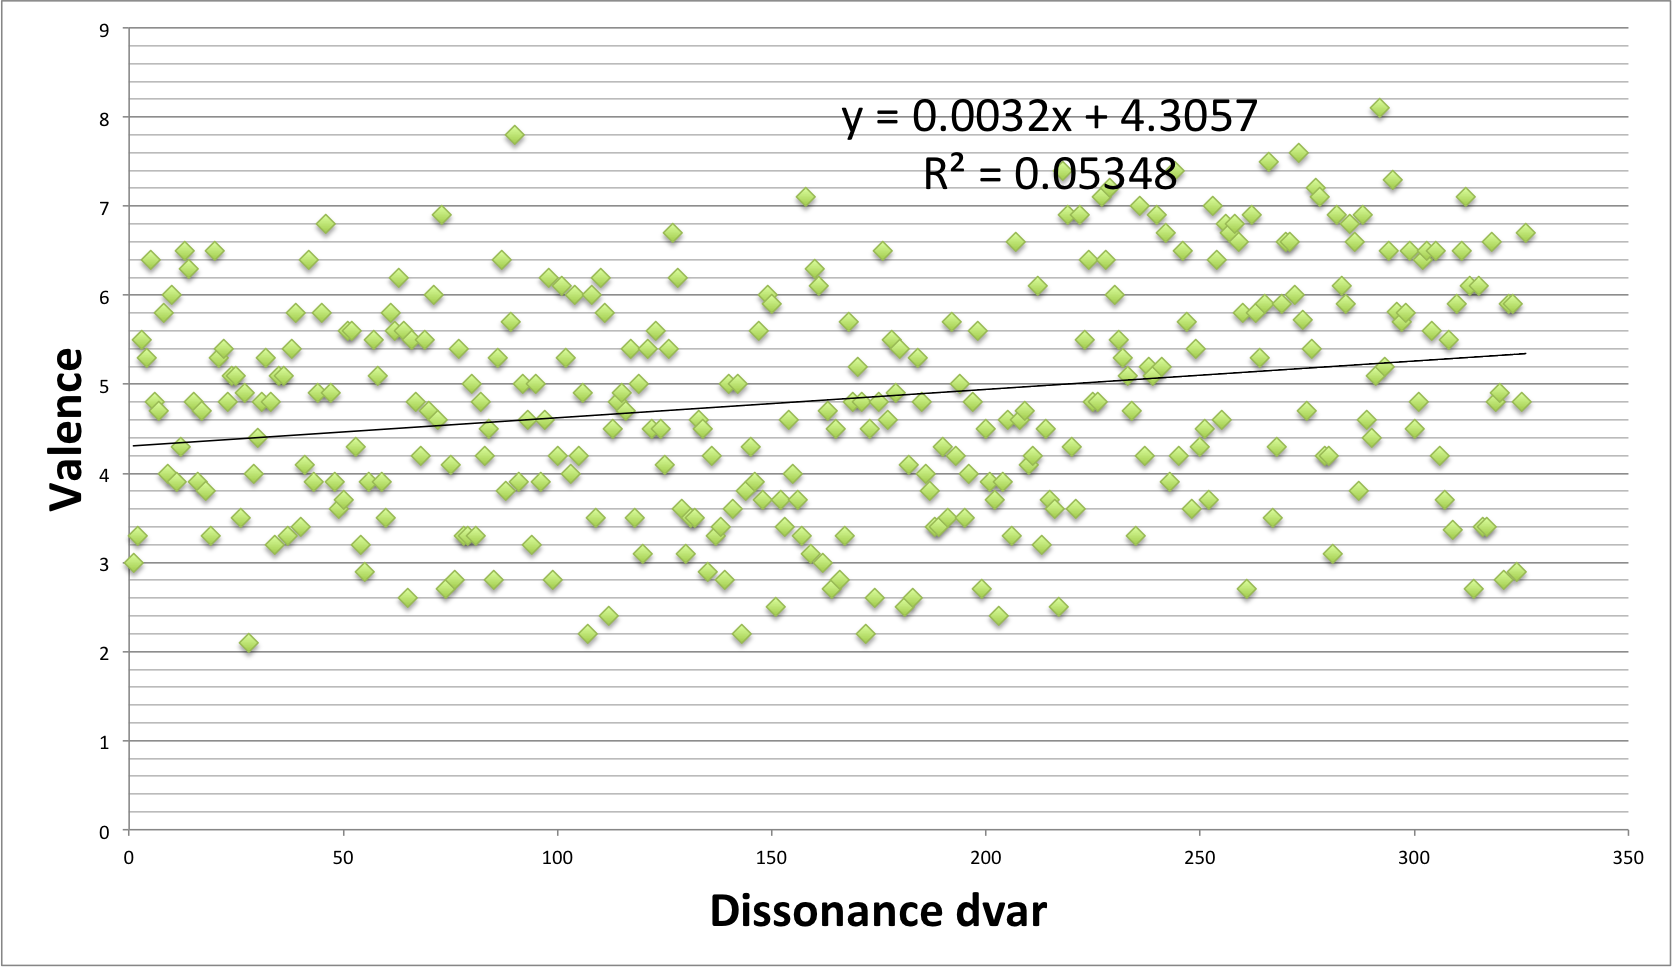
\includegraphics[width=\textwidth]{Figures/dissonancedvar-valence}
                  \vspace{20pt}
        \end{subfigure}        
        
    
        
\end{figure}